% Appendices of the journal version. Included from main.tex inside \begin{appendices}.

\section{Overview and status labels}
\label{app:overview}
\Cref{app:exact} gives full proofs of \cref{sec:exact} (including
\cref{rem:sharp}), \cref{app:enum} the exhaustive enumeration check,
\cref{app:aggstate,app:agg} the statements and proofs for \cref{sec:agg}, \cref{app:finite} the proofs of
\cref{sec:finite} (including the plug-in effective sample size and the scope
of the recovery bound), \cref{app:sims} the simulation checks of F1--F3,
\cref{app:lean} the map from statements to Lean names, \cref{app:real} data
selection and preprocessing for the real-data studies, \cref{app:estimand}
the real-data estimand $\tilde s$, \cref{app:prereg} the analysis-plan
timeline for all studies and experiments, prior exposure and deviations,
\cref{app:e1,app:e2} the experiments E1 and E2 in full,
\cref{app:noloop,app:lags,app:er,app:x3} the loop-free graphs, lagged
unrollings, the random summary graphs (with the full proof of \cref{prop:er}
in \cref{app:erproof}) and the accuracy interpretation,
\cref{app:b1,app:b1nl,app:b1x,app:b3} the benchmark experiment B1, its
replication B1-NL, the extension to competitive learners with the post hoc
re-analysis, detectability calculation and generator survey, and the
discriminating test B3, and \cref{app:ident} the proofs of
\cref{sec:labels,sec:ident}.

Status labels. \emph{Machine-checked}: a Lean theorem with no \texttt{sorry}
and only the standard axioms. \emph{Proved}: a complete paper proof given
here. \emph{Asymptotic}: a limit statement proved here from the multivariate
Breuer--Major theorem \citep{arcones1994limit,nourdin2011quantitative} (cited, not
re-proved). \emph{Sketched}: a derivation with one analytic step left out,
stated as such (used only for statements outside the main claims: the windowed
loop-free stationary value, the layered-DAG stationary value and the constants
of the lagged recovery bound).
\emph{Enumerated}: checked by exact computation on many instances, not proved.

%=============================================================================
\section{Proofs for Section~\ref{sec:exact}}
\label{app:exact}


\textbf{Definition of $\srho$, verbatim.} \citet[Sec.~2.2]{reisach2026topological}
(arXiv v1) write: ``For a graph $G=(V,E)$ with $|E|\ge1$ we define sortability
by the number of relatives, or rel-sortability for short, as
$s_\rho(G):=\frac{\sum_{(x,y)\in E}s_\rho(x,y)}{|E|}$ with
$s_\rho(x,y):=0$ if $\rho(x)>\rho(y)$, $\frac12$ if $\rho(x)=\rho(y)$, $1$ if
$\rho(x)<\rho(y)$, for $(x,y)\in E$.'' (their Eq.~(4); the cases are typeset as a
brace there), and add: ``Note that our definition differs from the sortabilities
in these works in that we count edges instead of paths.'' Our $\srho$ is this
edge average; in $\GT$ the edges are the copies $(i(t),j(t{+}1))$.

Throughout, $\GS=(V,\Es)$ has a self-loop at every node, $p=|V|\ge2$, and
$d(u,v)$ is as in \cref{sec:setting}. We use two facts of
\citet{reisach2026topological}, proved there for DAGs: (Thm.~1) if
$x\in\anc(y)$ then $\rel(x)\subseteq\rel(y)$; (Lemma~1, eq.~(10)) if
$x\in\anc(y)$ then $\rel(x)\subsetneq\rel(y)$ iff $\mathrm{roots}(y)\setminus
\mathrm{roots}(x)\ne\emptyset$, where $\mathrm{roots}(y)=\{x\in\anc(y):\anc(x)=\{x\}\}$.
Both are also machine-checked independently
(\lname{relSet_subset_of_edge}, and the direct characterisation
\lname{isRel_unrolled_iff}).

\begin{lemma}[ancestors in $\GT$]\label{lem:anc}
$u(s)\in\anc(v(t))$ iff $s\le t$ and $d(u,v)\le t-s$.
\lean{\lname{unrolled_reach_iff}, \lname{unrolled_reach_iff_dist}.}
\end{lemma}
\begin{proof}
Every edge of $\GT$ increases time by one, so a directed path from $u(s)$ to
$v(t)$ has $t-s$ edges, and its projection to $V$ is a walk of length $t-s$
from $u$ to $v$ in $\GS$ (self-loops allowed as steps). Such a walk exists iff
$d(u,v)\le t-s$: a walk contains a path, so its length is at least
$d(u,v)$; conversely, pad a shortest path with $t-s-d(u,v)$ self-loop steps at
$u$. Every such walk lifts to a directed path in $\GT$.
\end{proof}

\begin{lemma}[roots]\label{lem:roots}
$\mathrm{roots}(v(t))=\{u(1):d(u,v)\le t-1\}$, and
$\desc(u(1))=\{w(s):d(u,w)\le s-1\}$.
\lean{\lname{roots_unrolled_iff}, \lname{isRoot_unrolled_iff}, \lname{desc_root_unrolled_iff}.}
\end{lemma}
\begin{proof}
A node $u(s)$ with $s\ge2$ has the parent $u(s-1)$ through the self-loop, so
it is not a root; $u(1)$ has no parent. Apply \cref{lem:anc} with $s=1$, in
both directions.
\end{proof}

\begin{proof}[Proof of \cref{thm:edge}]
$i(t)$ is a parent of $j(t{+}1)$, so $\rel(i(t))\subseteq\rel(j(t{+}1))$ and
$\srho(e)\in\{1/2,1\}$, with value $1$ iff the inclusion is strict, iff
$\mathrm{roots}(j(t{+}1))\setminus\mathrm{roots}(i(t))\neq\emptyset$. By
\cref{lem:roots} this set is $\{u(1):d(u,j)\le t,\ d(u,i)>t-1\}$, and since
$d$ is integer-valued or $\infty$, $d(u,i)>t-1$ iff $d(u,i)\ge t$.
\end{proof}

\begin{proof}[Proof of \cref{prop:boundary} (and the general count)]
Since every ancestor of $y$ descends from a root of $y$ that is itself an
ancestor, $\rel(y)=\desc(\mathrm{roots}(y))$. By \cref{lem:roots},
$w(s)\in\rel(v(t))$ iff some $u$ has $d(u,v)\le t-1$ and $d(u,w)\le s-1$,
i.e.\ iff $s\ge1+m_t(v,w)$ with $m_t(v,w)=\min\{d(u,w):d(u,v)\le t-1\}$.
Counting $s\in\{1,\dots,T\}$ gives
$\rho(v(t))=\sum_{w}\max(T-m_t(v,w),0)$ (\lname{rho_unrolled_eq}). For
$t\ge p$ every finite $d(u,v)$ is at most $p-1\le t-1$, so the admissible $u$
are $\anc_S(v)$ and $m_t(v,w)=d(\anc_S(v),w)$, finite iff $w\in\rel_S(v)$ and
then at most $p-1<t\le T$. (The Lean statement \lname{rho_unrolled_large_t}
needs only $t\ge p$; an earlier hypothesis $T\ge p$ is redundant.)
\end{proof}

\begin{proof}[Proof of \cref{thm:limit}]
Crossing edge $(i,j)\in\Ex$: $j$ does not reach $i$, so $d(j,i)=\infty$, and
$u=j$ gives $d(j,j)=0\le t\le\infty$ for every $t$: all $T-1$ copies score
$1$. Edge in $\Eo$: $i$ and $j$ reach each other (or $i=j$), so for every $u$,
$d(u,i)<\infty$ iff $d(u,j)<\infty$. If the condition of \cref{thm:edge} held
with $d(u,i)=\infty$ then $d(u,j)=\infty>t$, a contradiction; hence it forces
$t\le d(u,i)\le\Delta$, and at most $N_T(i,j)\le\min(\Delta,T-1)$ copies score
$1$ ($\Delta\le p-1$, \lname{maxFinDist_le_card_sub_one}). Summing over the $(T-1)|\Es|$ edges,
\[
\srho(\GT)=\tfrac12+\frac{1}{2(T-1)|\Es|}\Big[(T-1)|\Ex|+\sum_{(i,j)\in\Eo}N_T(i,j)\Big],
\]
which gives both bounds; let $T\to\infty$. Lean: \lname{sRho_unrolled_bounds_maxFinDist}
(the $\Delta$ form), with the $p-1$ form \lname{sRho_unrolled_bounds} as a corollary.
\end{proof}

\begin{proof}[Proof of \cref{cor:iff}]
$\Ex=\emptyset$ iff no edge joins two SCCs. A weakly connected component made of
two or more SCCs is connected by undirected edges, one of which joins two
different SCCs; conversely a strongly connected component has no crossing
edge. The uniform bound is \cref{thm:limit} with $|\Ex|\ge1$. For the DAG case,
every SCC is a singleton, $\Ex$ consists of the $m$ non-loop edges, and
$|\Es|=m+p$.
\end{proof}

\begin{proof}[Proof of \cref{thm:stat}]
In $G_{B+T}$, by \cref{lem:roots} shifted by $B$, $w(s)\in\rel(v(t))$ iff some
$u$ has $d(u,v)\le t-1$ and $d(u,w)\le s-1$. For window nodes $t-1,s-1\ge
B\ge\Delta$, and every finite distance is at most $\Delta$, so the condition is
$u\in\anc_S(v)\cap\anc_S(w)$, independent of $s,t$. Hence
$\rel_W(v(t))=\{w(s)\in W: w\in\rel_S(v)\}$, of size $T|\rel_S(v)|$. On
$V\times\mathbb Z$, \cref{lem:anc} holds verbatim and the common ancestor can
be taken arbitrarily early, giving the same set. Each copy of $(i,j)$ therefore
compares $|\rel_S(i)|$ with $|\rel_S(j)|$; as $i\in\anc_S(j)$,
$\rel_S(i)\subseteq\rel_S(j)$, so the score is $1$ iff
$\rel_S(i)\ne\rel_S(j)$, and $1/2$ for self-loops.
Source SCCs: $\rel_S(j)\setminus\rel_S(i)\ne\emptyset$ iff
$\anc_S(j)\not\subseteq\rel_S(i)$ (if $z\in\rel_S(i)$ then
$\desc_S(z)\subseteq\rel_S(i)$). Every node of $\anc_S(j)$ is reached from some
$\sigma\in\Src(j)$, and $\desc_S(\sigma)\subseteq\rel_S(i)$ whenever
$\sigma\subseteq\rel_S(i)$. A source SCC meets $\rel_S(i)$ iff it reaches $i$
(its only ancestors are its own nodes), and then it is contained in
$\rel_S(i)$. So the condition is $\Src(j)\not\subseteq\Src(i)$, which, as
$\Src(i)\subseteq\Src(j)$, is $\Src(i)\ne\Src(j)$. Lean:
\lname{rhoBurn_eq_maxFinDist}, \lname{sBurn_eq_maxFinDist} (with $B\ge\Delta$), and the
$B\ge p-1$ forms \lname{rhoBurn_eq}, \lname{sBurn_eq} as corollaries.
\end{proof}

\begin{remark}[sharpness of $B\ge\Delta$ for one edge]\label{rem:sharp}
For the single edge $0\to1$ with self-loops, $\Delta=1$; with $B=1$ the window
value is the stationary value $1/2$, and with $B=\Delta-1=0$ it is at least
$2/3$ for every $T\ge2$ (\lname{edgeLoops_burn_sharp}). So $B\ge\Delta$ cannot be
lowered for this graph. This is all that is proved. Enumeration on 726 random
summary graphs gave the stationary value at $B=\Delta$ in all of them, and at
$B=\Delta-1$ in 281; in 445 it did not (\cref{app:b1}). Hence $\Delta-1$
suffices for some graphs, and the minimal sufficient burn-in of a given graph
can be shorter than $\Delta$. We have no proof that for every $\Delta\ge2$ some
graph needs exactly $\Delta$ slices, and no closed form for the minimal
burn-in. Proving the first, for instance for the directed chain with
self-loops, would turn the enumeration into a theorem.
\end{remark}

\begin{proof}[Proof of \cref{cor:statiff}]
If each weak component $C$ has a unique source SCC $\sigma_C$, then
$\Src(v)=\{\sigma_C\}$ on $C$ and $\Eu=\emptyset$. Conversely, if
$\Eu=\emptyset$, $\Src$ is constant along edges and hence on each weak
component; a node $v$ of a source SCC $\sigma$ has $\Src(v)=\{\sigma\}$, so
there is only one. Out-forests (at most one parent besides itself; acyclicity
is not needed, \lname{stat_half_of_outForest}) and strongly connected graphs
(\lname{stat_half_of_strong}) have one source SCC per component. In an
in-forest (acyclic apart from self-loops, out-degree at most one), if
$u\in\anc(v)$ then $\desc(u)$ is the unique downstream path through $v$, so
$\rel(v)=\anc(v)\cup\desc(v)$ (\lname{inForest_isRel_iff}); the source SCCs
are the headwaters, and $\Src(j)=\Src(i)\cup\bigcup_{k}\Src(k)$ over the other
parents $k$ of $j$, with disjoint headwater sets on different branches, so
$\Src(j)\ne\Src(i)$ iff $j$ is a confluence (\lname{inForest_up_iff}).
Out-degree at most one alone is not enough: for $a\rightleftarrows b$ with
$c\to a$, $a$ has two parents but the only source SCC is $\{c\}$.
\end{proof}

\begin{remark}[self-loops]
Without self-loops the lemmas fail: for the single edge $0\to1$ without loops,
$\srho(\GT)=1/2$ for every $T\ge2$ (\lname{edgeNoLoops_sRho}); with loops the
limit is $2/3$ (\lname{edgeLoops_limit}).
\end{remark}

%=============================================================================
\section{Exhaustive Enumeration Check}
\label{app:enum}

Before formalisation, every statement of \cref{sec:exact} was checked by
brute force (bitset relatives with the definitions of
\citealp{reisach2026topological}) on all $4+64+4096$ summary graphs with
$p=2,3,4$ (all $T\le9$) and on $10{,}000$ random graphs ($p=2$--$7$; Erd\H{o}s--R\'enyi,
DAG, in-forest, out-forest, chain with back edge and block-SCC families;
three values of $T\le14$ each, fixed seed). In total 46{,}724 (graph,~$T$)
cases and 1{,}895{,}609 edges were checked with zero failures of
\cref{thm:edge}, \cref{prop:boundary}, the bounds of \cref{thm:limit},
\cref{thm:stat} (with $B=p-1$ and $B=2p+1$) and the source-SCC
characterisation. The conjecture fixed in plan 1 (``an edge is strictly
sorted in the limit iff $|\rel_S(j)|>|\rel_S(i)|$'') disagreed with the exact
$\GT$ limit in 9{,}603 random graphs and never with the stationary value; the
conjecture is \cref{thm:stat}, not the limit of $\GT$.

%=============================================================================
%=============================================================================
\section{Block Means and Subsamples: Statements}
\label{app:aggstate}




For a stable linear SVAR with independent innovations, nodes with disjoint
summary ancestor sets are independent at all lags, and so are any per-node,
time-invariant transforms, including block means and subsamples; otherwise
the lag-0 covariance is nonzero for almost every parameter
(\cref{prop:zero}). So the population relatives of
contemporaneous values are $\rel_S$ for every observation scheme, and the
population relatives sort is the stationary value of \cref{thm:stat} (on
non-self-loop edges), not the finite-$\GT$ value. Var- and $R^2$-sortability
behave differently (\cref{thm:agg}): block means converge, at the textbook
Fej\'er rate for averages of a stationary series
\citep[Ch.~7]{brockwell1991time}, to the long-run structural model of
\citet{gong2017aggregated}, whereas subsamples keep the snapshot covariance. As a
consequence, for large block size, block-mean $R^2$-sortability is $0$ on
out-stars and $1$ on in-stars with at least two arms for all weights; on
out-stars subsampled data are $R^2$-sorted correctly on average ($0.84$) while
block means drift to $0$. We claim only these sortability consequences.


Assumptions: $X(t)=\sum_{\tau=1}^{L}A_\tau X(t-\tau)+\varepsilon(t)$, $t\in\mathbb Z$,
i.i.d.\ innovations with diagonal positive-definite covariance $\Sigma$, stable
(all roots of $\det(I-\sum_\tau A_\tau z^\tau)$ outside the unit disc),
stationary solution; the summary graph has $i\to j$ iff $(A_\tau)_{ji}\ne0$ for
some $\tau$. $\Gamma(h)$ is the autocovariance, $A(1)=\sum_\tau A_\tau$, and for a
block size $D$ the block means are $\bar Y_s=\frac1D\sum_{u<D}X(sD{+}u)$ and the
subsamples $Z_s=X(sD)$.

\begin{proposition}[relatives survive any per-node filter]\label{prop:zero}
If $\anc_S(i)\cap\anc_S(j)=\emptyset$ then $X_i$ and $X_j$ are independent at
all lags, and so are any per-node, time-invariant (possibly nonlinear)
transforms of them, including $\bar Y$ and $Z$ for every $D$. If the
ancestor sets intersect, $\Gamma(0)_{ij}$, $\mathrm{Cov}(\bar Y)_{ij}$ and the
long-run covariance are nonzero for Lebesgue-almost every parameter.
\nolean{needs the SVAR moving-average representation and real-analytic genericity}
\end{proposition}

\begin{theorem}[block means vs subsampling]\label{thm:agg}
(a) $\|D\,\mathrm{Cov}(\bar Y)-S_{LR}\|\le\frac1D\sum_h|h|\|\Gamma(h)\|$,
with $S_{LR}=(I-A(1))^{-1}\Sigma(I-A(1))^{-\top}$.
(b) If $\GS$ is acyclic apart from self-loops, $S_{LR}$ is the covariance of a
static SEM (this long-run SEM is due to \citealp[Eqs.~(5), (10)]{gong2017aggregated}) on $\GS$ with weights $A(1)_{ji}/(1-\lambda_j)$ and noise variances
$\sigma_j^2/(1-\lambda_j)^2$, $\lambda_j=A(1)_{jj}<1$.
(c) $\mathrm{Cov}(Z_s)=\Gamma(0)$ for every $D$.
(d) Hence, for large $D$, block-mean $R^2$-sortability is $0$ on out-stars and
$1$ on in-stars with $\ge2$ arms, for all weights; under subsampling every
contemporaneous criterion keeps its $\Gamma(0)$ value.
\lean{(a) counting identity \lname{fejer_identity}; (b) \lname{longrun_factor}, \lname{selfloop_sum_lt_one}; the probabilistic steps, the rate and (c)--(d) are not machine-checked.}
\end{theorem}
Part (a) is the standard Fej\'er/Ces\`aro computation for the variance of the
mean of a stationary series \citep[Ch.~7]{brockwell1991time}, written for
block means of a vector process; (b) is due to \citet{gong2017aggregated}; (c)
is stationarity. We claim only the sortability consequences (d).

The $R^2$ statement for stars strengthens the three-node analysis in
\citet[App.~D]{herman2025unitless}, whose qualitative message (that $R^2$
reflects connectivity, with an asymmetry between colliders and confounders)
we credit. Numerical observations (exact population moments, not proved):
mean block-mean $R^2$-sortability over 150 in-trees moves from $0.853$
($D=1$) to $0.834$ ($D=4$--$8$) and $0.880$ ($D=256$), so it is not monotone in
$D$; on out-stars subsampled data are $R^2$-sorted at $0.842$ on average while
block means give $0.546$ ($D=4$), $0.101$ ($D=16$) and $0$ in the limit.


\section{Proofs for the Block-Mean and Subsampling Statements}
\label{app:agg}

\begin{proof}[Proof of \cref{prop:zero}]
By the MA($\infty$) representation $X(t)=\sum_k\Psi_k\varepsilon(t-k)$, and
because $\Psi_k$ is supported on the reachability relation, $X_i(t)$ is a
measurable function of $\{\varepsilon_k(s):k\in\anc_S(i)\}$. Disjoint ancestor
sets mean independent innovation sets, so the processes $X_i$ and $X_j$ are
independent, and so are any per-node transforms. For the generic part, each
covariance entry is real-analytic in $(A,\Sigma)$ on the connected open set of
stable parameters with the given support, hence either identically zero or
nonzero almost everywhere. With all coefficients positive, including the
self-loop at a common ancestor $k$, all $\Psi$ entries are nonnegative and
$\Psi_{ik}(m),\Psi_{jk}(m)>0$ for all large $m$ (self-loops pad the walks), so
$\Gamma(0)_{ij}>0$; the same holds for $\Gamma(h)$, $h\ge0$, and therefore for
the Fej\'er sums and $S_{LR}$. ``Generic'' does not mean ``large'': with little
autocorrelation, $\Gamma(0)_{ij}$ along a lagged edge can be tiny (down to
$10^{-14}$ in our exact computations; exactly $0$ without autocorrelation).
\end{proof}

\begin{proof}[Proof of \cref{thm:agg}]
(a) $D^2\mathrm{Cov}(\bar Y)=\sum_{u,w<D}\Gamma(u-w)=D\Gamma(0)+\sum_{h=1}^{D-1}(D-h)(\Gamma(h)+\Gamma(-h))$
(the counting identity is \lname{fejer_identity}). The stable VAR has
$\|\Gamma(h)\|\le C r^{|h|}$, $r<1$, so $\sum_h|h|\|\Gamma(h)\|<\infty$ and
$S_{LR}=\sum_h\Gamma(h)=\Psi(1)\Sigma\Psi(1)^\top$ with
$\Psi(1)=(I-A(1))^{-1}$. Then
$S_{LR}-D\,\mathrm{Cov}(\bar Y)=\sum_{|h|\ge D}\Gamma(h)+\sum_{|h|<D}\frac{|h|}{D}\Gamma(h)$,
and $1\le|h|/D$ in the first sum.
(b) Write $I-A(1)=(I-\Lambda)-N$ with $\Lambda$ the diagonal and $N$ the
off-diagonal part; then $I-A(1)=(I-\Lambda)(I-\tilde B)$ with
$\tilde B=(I-\Lambda)^{-1}N$ strictly triangular in a topological order
(\lname{longrun_factor}, \lname{longrun_inv}). Under acyclicity the AR
polynomial factorises into univariate $\phi_j(z)=1-\sum_\tau(A_\tau)_{jj}z^\tau$;
stability, $\phi_j(0)=1$ and the intermediate value theorem give
$\phi_j(1)=1-\lambda_j>0$ (\lname{selfloop_sum_lt_one}).
(c) Stationarity.
(d) For a linear SEM $X=BX+e$ with noise variances $\omega$,
$R^2_i=1-1/(\Sigma_{ii}(\Sigma^{-1})_{ii})$ and
$(\Sigma^{-1})_{ii}=1/\omega_i+\sum_{k\in\mathrm{ch}(i)}B_{ki}^2/\omega_k$. In
an out-star with root $0$ and leaves $k$, $1-R^2_0=1/(1+\sum_kr_k)$ and
$1-R^2_k=1/(1+r_k)$ with $r_k=\omega_0B_{k0}^2/\omega_k>0$, so with $\ge2$
leaves the root has strictly larger $R^2$ than every leaf; the in-star is
symmetric. Strict inequalities in the limit SEM of (b), plus (a) and
continuity of $S\mapsto R^2$ at positive-definite $S$, give the claim for all
large $D$. Under subsampling every contemporaneous statistic is a function of
$\Gamma(0)$.
\end{proof}

%=============================================================================
\section{Proofs for Section~\ref{sec:finite}}
\label{app:finite}

Notation. $\hat C_{ab}=\frac1n\sum_t(X_a(t)-\bar X_a)(X_b(t)-\bar X_b)$,
$\hat r_{ab}=\hat C_{ab}/\sqrt{\hat C_{aa}\hat C_{bb}}$. Constants:
$B_{ab}$ as in the main text; $D_\gamma=\max_a2\sum_h\gamma_{aa}(h)^2$;
$\kappa_1=\max_a\sum_h|\gamma_{aa}(h)|$;
$\kappa_2=\max_{a\ne b}(\sum_h|\gamma_{aa}(h)|+\sum_h|\gamma_{ab}(h)|)$. For
i.i.d.\ sampling, $B_{ab}=1+\rho_{ab}^2$, $D_\gamma=2$, $\kappa_1=1$.

\begin{lemma}[Gaussian chaos tail]\label{lem:chaos}
Let $g\sim N(0,I_N)$, $A$ symmetric, $S=g^\top Ag-\mathrm{tr}A$. For $x>0$,
$P(S\ge2\|A\|_F\sqrt x+2\|A\|_{op}x)\le e^{-x}$, and the same for $-S$.
\lean{algebraic steps \lname{phi_le}, \lname{chernoff_logmgf_le}, \lname{chernoff_choice}, \lname{sqrt_two_v_x}; the probability statement is not machine-checked.}
\end{lemma}
\begin{proof}
Diagonalise; $S$ has the law of $\sum_i\lambda_i(g_i^2-1)$. For $2s\lambda<1$,
$\log Ee^{s\lambda(g^2-1)}=\varphi(s\lambda)$ with
$\varphi(u)=-\frac12\log(1-2u)-u=\sum_{k\ge2}(2u)^k/(2k)\le u^2/(1-2|u|)$ for
$|u|<1/2$. With $c=2\|A\|_{op}$, $v=2\|A\|_F^2$ and $0\le s<1/c$,
$\log Ee^{sS}\le vs^2/(2(1-cs))$. Markov's inequality with $t=\sqrt{2vx}+cx$,
$q=\sqrt{2x/v}$ and $s=q/(1+cq)$ gives exponent exactly $x$. This is the
Gaussian case of \citet[Prop.~1]{hsu2012tail}, who derive it from
\citet{laurent2000adaptive}; the proof here is self-contained.
\end{proof}

\begin{lemma}[exact variance]\label{lem:var}
With $\tilde\gamma_{ab}=\frac1n\sum_tX_a(t)X_b(t)=g^\top Ag$ for
$A=C^{1/2}MC^{1/2}$, $M=\frac1{2n}\begin{psmallmatrix}0&I\\I&0\end{psmallmatrix}$,
\[
2n\|A\|_F^2=\sum_{|h|<n}\Big(1-\tfrac{|h|}{n}\Big)\big[\gamma_{aa}(h)\gamma_{bb}(h)+\gamma_{ab}(h)\gamma_{ab}(-h)\big]\le B_{ab},
\]
$\|A\|_{op}\le\kappa_2/(2n)$; on the diagonal $2n\|A\|_F^2\le D_\gamma$ and
$\|A\|_{op}\le\kappa_1/n$; and $\bar X_a\sim N(0,\bar\sigma_a^2)$ with
$\bar\sigma_a^2\le\kappa_1/n$.
\lean{trace and Toeplitz algebra \lname{quad_M}, \lname{trace_MC}, \lname{lemma12_trace}, \lname{lemma12_fejer}, \lname{lemma12_le_B}, \lname{lemma12_diag_le_D}; the step $\|C^{1/2}MC^{1/2}\|_F^2=\mathrm{tr}(MCMC)$ and the operator-norm bounds are not machine-checked.}
\end{lemma}
\begin{proof}
$\|A\|_F^2=\mathrm{tr}(MCMC)$ and, with Toeplitz blocks
$(C_{ab})_{st}=\gamma_{ab}(s-t)$,
$4n^2\mathrm{tr}(MCMC)=2\sum_{s,t}[\gamma_{aa}(s-t)\gamma_{bb}(s-t)+\gamma_{ab}(s-t)\gamma_{ab}(t-s)]$
(using that $\gamma_{aa}$, $\gamma_{bb}$ are even); count pairs with $s-t=h$.
$\|A\|_{op}\le\|C\|_{op}\|M\|_{op}$ and $\|C\|_{op}$ is at most the largest
absolute row sum.
\end{proof}

\begin{lemma}[deviation event]\label{lem:dev}
Let $\varepsilon_{ab}=\sqrt{2B_{ab}x/n}+\kappa_2x/n+2\kappa_1y/n$ and
$\varepsilon_d=\sqrt{2D_\gamma y/n}+4\kappa_1y/n$. With probability at least
$1-d(d{-}1)e^{-x}-4de^{-y}$, $|\hat C_{ab}-\rho_{ab}|\le\varepsilon_{ab}$ for all
$a\ne b$ and $|\hat C_{aa}-1|\le\varepsilon_d$ for all $a$.
\lean{deterministic steps \lname{centred_cov_eq}, \lname{centred_dev_offdiag}, \lname{centred_dev_diag}, \lname{lemma13_eps}, \lname{lemma13_count}.}
\end{lemma}
\begin{proof}
$\hat C_{ab}=\tilde\gamma_{ab}-\bar X_a\bar X_b$. Apply \cref{lem:chaos,lem:var}
to each off-diagonal and diagonal $\tilde\gamma$, bound $|\bar X_a|\le
\sqrt{2\kappa_1y/n}$ by the Gaussian Chernoff bound, and take a union bound.
\end{proof}

\begin{lemma}[correlation perturbation]\label{lem:pert}
If $a',b'\in[1-\varepsilon_d,1+\varepsilon_d]$, $\varepsilon_d<1$ and
$|c'-\rho|\le\varepsilon$, then
$|c'/\sqrt{a'b'}-\rho|\le(\varepsilon+|\rho|\varepsilon_d)/(1-\varepsilon_d)$.
\lean{\lname{corr_perturb} (the hypothesis $|\rho|\le1$ of our earlier statement is not needed).}
\end{lemma}
\begin{proof}
$|c'/\sqrt{a'b'}-\rho|\le|c'-\rho|/\sqrt{a'b'}+|\rho||1/\sqrt{a'b'}-1|$, with
$1/\sqrt{a'b'}\le1/(1-\varepsilon_d)$ and $|1/\sqrt{a'b'}-1|\le\varepsilon_d/(1-\varepsilon_d)$.
\end{proof}

\begin{theorem}[recovery bound]\label{thm:f1}
For $x,y>0$ let $\varepsilon_{ab}$, $\varepsilon_d<1$ be as in \cref{lem:dev} and
$\delta_{ab}=(\varepsilon_{ab}+|\rho_{ab}|\varepsilon_d)/(1-\varepsilon_d)$. If
thresholds separate ($\delta_{ab}\le\tau_{ab}$ on non-relatives and
$|\rho_{ab}|-\delta_{ab}>\tau_{ab}$ on relatives), the declared set equals the true
one, and hence $\hat s=\srho^{\mathrm{pop}}$, with probability at least
$1-d(d{-}1)e^{-x}-4de^{-y}$. For a common threshold $\tau<\rho_{\min}$ the
failure probability decays as
$\exp(-n\min(\tau,\rho_{\min}-\tau)^2/(2(\sqrt B+\rho_{\max}\sqrt{D_\gamma})^2))$.
\lean{deterministic core \lname{thm15_det}, \lname{decide_eq_target}, \lname{corr_perturb}, \lname{sOf_cntDecl_congr}; Chernoff and trace algebra \lname{chernoff_choice}, \lname{phi_le}, \lname{lemma12_trace}, \lname{lemma12_le_B}. The Gaussian tail bound itself is not machine-checked.}
\end{theorem}
The proof combines a Gaussian-chaos tail bound (the Gaussian case of
\citealp[Prop.~1]{hsu2012tail}; see also \citealp{laurent2000adaptive}), an exact
finite-$n$ variance identity for $\hat r$, and a deterministic perturbation
lemma.

\begin{proof}[Proof of \cref{thm:f1}]
Set $\delta_{ab}=(\varepsilon_{ab}+|\rho_{ab}|\varepsilon_d)/(1-\varepsilon_d)$.
On the event of \cref{lem:dev}, \cref{lem:pert} gives
$|\hat r_{ab}-\rho_{ab}|\le\delta_{ab}$, so non-relatives satisfy
$|\hat r|\le\tau$ and relatives $|\hat r|>\tau$ (\lname{decide_eq_target},
\lname{thm15_det}). Equal declared sets give equal counts and hence
$\hat s=\srho^{\mathrm{pop}}$ (\lname{sOf_cntDecl_congr}). For a VAR observed
as a long stationary series, $\srho^{\mathrm{pop}}$ is the stationary value
of \cref{thm:stat} on non-self-loop edges (\cref{prop:zero}). Explicit form:
with $y=x+\log(4/(d-1))_+$ (\lname{explicit_y}) and a common threshold
$\tau<\rho_{\min}$,
$P(\hat R\ne R)\le2d(d{-}1)\exp\!\big(-n\min(\tau,\rho_{\min}-\tau)^2/(2(\sqrt B+\rho_{\max}\sqrt{D_\gamma})^2)(1+o(1))\big)$.
\end{proof}

\textbf{The multivariate Breuer--Major theorem.} We use it in the form stated
by \citet[Thm.~1.1]{nourdin2011quantitative}, who attribute the vector case to
\citet{arcones1994limit}: let $X=(X_k)_{k\in\mathbb Z}$ be a centred stationary
Gaussian process in $\mathbb R^d$ with covariances $r^{(i,l)}(j)=E[X^{(i)}_1X^{(l)}_{1+j}]$,
and $f:\mathbb R^d\to\mathbb R$ with $E f(X_1)^2<\infty$ and Hermite rank $q\ge1$
with respect to $X$ (orthogonal to all polynomials of degree $<q$, not to some of
degree $q$). If $\sum_{j\in\mathbb Z}|r^{(i,l)}(j)|^q<\infty$ for all $i,l$, then
$n^{-1/2}\sum_{k\le n}(f(X_k)-Ef(X_k))\Rightarrow N(0,\sigma^2)$ with
$\sigma^2=\mathrm{Var}f(X_1)+2\sum_{k\ge1}\mathrm{Cov}(f(X_1),f(X_{1+k}))\in[0,\infty)$.

\begin{proof}[Proof of \cref{prop:nominal}]
Take $d=2$, $X_k=(X_a(k),X_b(k))$ and, for $c\in\mathbb R^3$,
$f_c(x)=c_1(x_a^2-1)+c_2(x_b^2-1)+c_3(x_ax_b-\rho_{ab})$. $f_c$ is a centred
polynomial of degree $2$ without linear part, so it is orthogonal to every
polynomial of degree $\le1$ (odd Gaussian moments vanish); if it were orthogonal
to every polynomial of degree $2$ it would be orthogonal to itself, so either
$f_c(X_1)=0$ a.s.\ (then the partial sums vanish) or its Hermite rank is $2$.
The condition $\sum_h|\gamma_{ab}(h)|^2<\infty$ holds because the covariances are
absolutely summable and bounded. By the theorem and the Cram\'er--Wold device,
$\sqrt n(\tilde\gamma_{aa}-1,\tilde\gamma_{bb}-1,\tilde\gamma_{ab}-\rho_{ab})\Rightarrow N(0,V)$,
where, by Isserlis' theorem, $V(ab,cd)=\sum_h[\gamma_{ac}(h)\gamma_{bd}(h)+\gamma_{ad}(h)\gamma_{bc}(h)]$
(as in \cref{lem:var}). Centring by the sample means changes each entry by
$\bar X_a\bar X_b$, and $\sqrt n\bar X_a\bar X_b\to0$ in probability since
$E(\sqrt n\bar X_a)^2\le\kappa_1$ and $\bar X_b\to0$; Slutsky's lemma applies.
The delta method with gradient $(-\rho/2,-\rho/2,1)$ gives $\sqrt n(\hat r-\rho)
\Rightarrow N(0,W)$,
$W=V(ab,ab)-\rho[V(ab,aa)+V(ab,bb)]+\frac{\rho^2}{4}[V(aa,aa)+2V(aa,bb)+V(bb,bb)]$,
which equals $\sum_h\gamma_{aa}(h)\gamma_{bb}(h)$ for an independent pair (this is
$B_{ab}$ when all products $\gamma_{aa}(h)\gamma_{bb}(h)$ are nonnegative, and at most
$B_{ab}$ in general). Then $\sqrt{n}\,\atanh\hat r\Rightarrow N(0,W_{ab})$ under the
null and $P(|\atanh\hat r|>z_c/\sqrt{n-3})\to2\bar\Phi(z_c/\sqrt{W_{ab}})$, which
exceeds the nominal $\alpha/m$ in the limit whenever $W_{ab}>1$.
\end{proof}

\begin{lemma}[sample autocovariances]\label{lem:acvl2}
Let $X_a$ be a standardised stationary Gaussian series with $\sum_h|\gamma_{aa}(h)|\le\kappa_1$ and
$\hat\gamma_a(h)=\frac1n\sum_{t\le n-h}(X_a(t{+}h)-\bar X_a)(X_a(t)-\bar X_a)$. For $0\le h<n$,
$E(\hat\gamma_a(h)-\gamma_{aa}(h))^2\le(8\kappa_1+108\kappa_1^2)/n+2(h/n)^2\gamma_{aa}(h)^2$.
\end{lemma}
\begin{proof}
For $\tilde\gamma(h)=\frac1n\sum_{t\le n-h}X(t{+}h)X(t)$, $E\tilde\gamma(h)=(1-h/n)\gamma(h)$ and, by Isserlis,
$\mathrm{Var}\,\tilde\gamma(h)=n^{-2}\sum_{s,t\le n-h}[\gamma(s{-}t)^2+\gamma(s{-}t{+}h)\gamma(s{-}t{-}h)]\le2\kappa_1/n$,
since $|\gamma|\le1$ gives $\sum_k\gamma(k)^2\le\kappa_1$ and $\sum_k|\gamma(k{+}h)\gamma(k{-}h)|\le\kappa_1$. The
centring term is $-\bar X(S_1+S_2)/n+\frac{n-h}{n}\bar X^2$ with $S_1,S_2$ partial sums; $\bar X$, $S_1/n$, $S_2/n$ are
centred Gaussians with variance $\le\kappa_1/n$ and $E(UV)^2\le3\sigma^4$ for such pairs, so its second moment is
$\le27\kappa_1^2/n^2$. Combine with $(u+v+w)^2\le4u^2+4v^2+2w^2$ for $u+v$ and the bias $w=h\gamma(h)/n$.
\end{proof}

\begin{lemma}[plug-in Bartlett factor]\label{lem:plugin}
Let $X_a,X_b$ satisfy the assumptions of \cref{sec:finite} (no condition on their cross-dependence),
$\hat\rho_a(h)=\hat\gamma_a(h)/\hat\gamma_a(0)$, $\hat W_n=1+2\sum_{h=1}^{K_n}\hat\rho_a(h)\hat\rho_b(h)$ and
$W^\circ_{ab}=\sum_{h\in\mathbb Z}\rho_a(h)\rho_b(h)$. If $K_n\to\infty$ and $K_n/n\to0$, then
$|\hat W_n-W^\circ_{ab}|=O_P(n^{-1/2}+K_n/n)+2\sum_{h>K_n}|\rho_a(h)\rho_b(h)|\to0$; for fixed $K$,
$\hat W\to1+2\sum_{h\le K}\rho_a(h)\rho_b(h)$ in probability.
\end{lemma}
\begin{proof}
With $\Delta_a=\hat\rho_a-\rho_a$, on $\{\hat\gamma_a(0),\hat\gamma_b(0)\ge\frac12\}$ (probability $\to1$),
$|\Delta_a(h)|\le2|\hat\gamma_a(h)-\gamma_{aa}(h)|+2|\gamma_{aa}(h)||\hat\gamma_a(0)-1|$. Write
$\hat\rho_a\hat\rho_b-\rho_a\rho_b=\Delta_a\rho_b+\rho_a\Delta_b+\Delta_a\Delta_b$. By \cref{lem:acvl2},
$E\sum_{h\le K}|\hat\gamma_a(h)-\gamma_{aa}(h)||\rho_b(h)|\le\kappa_1\sqrt{c_0/n}+\sqrt2\kappa_1K/n$, so the linear terms
are $O_P(n^{-1/2}+K/n)$; by Cauchy--Schwarz and $E\sum_{h\le K}(\hat\gamma_a-\gamma_{aa})^2\le Kc_0/n+2\kappa_1(K/n)^2$,
$\sum_{h\le K}|\Delta_a\Delta_b|=O_P(K/n)$; the tail is at most $\sum_{h>K}|\rho_a(h)|\to0$.
\end{proof}
Only $K_n=o(n)$ is needed, because the target is a sum of products of two summable sequences; we do not rely on
general HAC bandwidth conditions.

\begin{proposition}[plug-in effective sample size]\label{prop:plugin}
Under the assumptions of \cref{prop:nominal}, use the plug-in threshold $\tanh(z_c/\sqrt{n/\hat B_{ab}-3})$ with
$\hat B_{ab}=\max(1,\hat W_n)$, where $1\le K_n=o(n)$.
(i) For an independent pair with $W_{ab}>0$ and $K_n\to\infty$, the false-positive probability tends to
$2\bar\Phi(z_c\sqrt{\max(1,W_{ab})/W_{ab}})$, which is $\alpha/m$ if $W_{ab}\ge1$ and smaller otherwise. For fixed $K$ it
tends to $2\bar\Phi(z_c\sqrt{\max(1,W^\circ_{K,ab})/W_{ab}})$, $W^\circ_{K,ab}=1+2\sum_{h\le K}\rho_a(h)\rho_b(h)$.
(ii) Every pair with $\rho_{ab}\ne0$ is declared with probability $\to1$.
(iii) If the non-relatives are independent pairs (summary non-relatives of a Gaussian VAR) and every relative has
$\rho_{ab}\ne0$, then $\liminf_nP(\hat R=R)\ge1-|N|\alpha/m\ge1-\alpha$, and the same holds for
$P(\hat s=\srho^{\mathrm{pop}})$, provided $K_n\to\infty$.
\nolean{uses the multivariate Breuer--Major theorem through \cref{prop:nominal}}
\end{proposition}
\begin{proof}
(i) $T=|\sqrt n\,\atanh\hat r|\,(1/\hat B-3/n)^{1/2}$. By \cref{prop:nominal}, $\sqrt n\,\atanh\hat r\Rightarrow N(0,W)$,
and $\hat B\to b=\max(1,W)$ (or $\max(1,W^\circ_K)$) in probability by \cref{lem:plugin}. By Slutsky,
$T\Rightarrow|N(0,W/b)|$, whose law has no atom at $z_c$. (ii) By \cref{lem:var}, $\hat r_{ab}\to\rho_{ab}$ in
probability. By Cauchy--Schwarz $|\hat\rho_a(h)|\le1$, so $\hat B\le1+2K_n=o(n)$ and $n/\hat B\to\infty$.
(iii) Union bound over $N$ with (i), and (ii) on $R$; equal declared sets give equal $\hat s$.
\end{proof}

\begin{proposition}[scope of \cref{thm:f1}]\label{prop:f1scope}
Let the non-relatives $N\neq\emptyset$ have deterministic thresholds with $n\tau_{n,ab}^2\to t_{ab}^2\in(0,\infty)$:
$t^2=z_c^2$ for the nominal Fisher-$z$ test, and $t^2=z_c^2b_{ab}$ for the effective one with $n'=n/b_{ab}$. Then the
smallest failure probability certified by \cref{thm:f1} tends to $d(d{-}1)\exp(-\min_Nt_{ab}^2/(2B_{ab}))>0$ when the
relatives have $|\rho|\ge\rho_{\min}>0$ (and is at least this in general). For i.i.d.\ data and the nominal test this
is $d(d{-}1)e^{-z_c^2/2}\ge\sqrt{2\pi}\,z_c\alpha$ (Mills), e.g.\ $0.089$ for $d=5$, $\alpha=0.01$. If instead
$\alpha_n\to0$ with $\log(1/\alpha_n)=o(n)$, \cref{thm:f1} gives
$P(\hat R\ne R)\le d(d{-}1)\exp(-(1-\eta)z_{c,n}^2r/2)+4d/n\to0$ for any $\eta>0$ and large $n$, with
$r=\min_N(n/n'_{ab})/B_{ab}$.
\end{proposition}
\begin{proof}
For $\rho_{ab}=0$ the separation condition $\delta_{ab}\le\tau_{n,ab}$ and $\varepsilon_{ab}\ge\sqrt{2B_{ab}x/n}$ force
$x\le n\tau_{n,ab}^2/(2B_{ab})$, which gives the lower bound. For attainment, take
$x_n=(1-\eta)\min_Nn\tau_{n,ab}^2/(2B_{ab})$ and $y_n=\log n$. Then all lower-order terms are $o(n^{-1/2})$ and
$\varepsilon_d\to0$, so the conditions hold for large $n$ on $N$, and on the relatives because $\tau_n\to0$. The
vanishing-level statement is the same computation with $z_{c,n}\to\infty$.
\end{proof}

\begin{remark}[non-Gaussian innovations]\label{rem:nongauss}
Let $X(t)=\sum_j\Psi_j\varepsilon(t-j)$ with $\sum_j\|\Psi_j\|<\infty$ and i.i.d.\ innovations with independent
unit-variance coordinates and fourth cumulants $\kappa_i=E\varepsilon_i^4-3$. Put
$G_i(a,b)=\sum_j\Psi_j[a,i]\Psi_j[b,i]$. Then $n\,\mathrm{Cov}(\tilde\gamma_{ab},\tilde\gamma_{cd})\to
V(ab,cd)+\sum_i\kappa_iG_i(a,b)G_i(c,d)$ (moment--cumulant formula and dominated convergence), so
$W_{ab}^{\mathrm{ng}}=W_{ab}+\sum_i\kappa_ig_i^2$ with $g_i=G_i(a,b)-\frac{\rho_{ab}}2(G_i(a,a)+G_i(b,b))$. Independent
series share no innovation, so $g_i=0$: the null variance $\sum_h\rho_a(h)\rho_b(h)$, and hence
\cref{prop:nominal,prop:plugin}, are unchanged, given the CLT for linear processes, which we do not re-prove. For
relatives, $W$ changes by $\sum_i\kappa_ig_i^2$ (of either sign, since $\kappa_i\ge-2$). This affects power and
transition widths, not the population statements or the location of $\nhalf$. The non-asymptotic bounds use the
Gaussian chaos tail. For sub-Gaussian innovations the Hanson--Wright inequality
\citep[Thm.~1.1]{rudelson2013hanson} has the same form with unspecified constants.
\end{remark}

\textbf{Fixed $K$ in practice (simulation and data check).} Independent AR(1)
pairs, 4{,}000 replications (2{,}000 at $n=64{,}000$): at AR coefficient
$0.9$ and $0.97$ the plug-in test with $K=50$ has size $0.050$ and $0.056$
(level $0.05$; limits $0.05$ and $0.0556$), but at $0.99$ it has $0.113$
(limit $0.118$), while $K_n=n^{0.6}$ gives $0.0495$ and the nominal test
$0.853$; for the opposite-sign pair the floor makes the test conservative
(size $0$). On the B3 primary data (30 segments of 3{,}000 rows, 2{,}730
unit-pairs) the declared status of no pair changes when $K=50$ is replaced
by $55$, $122$ or $300$ (post hoc). This was not checked for study 3, E1 or
the river data. Scripts: \texttt{finite2/}.


\textbf{F2 and F3.} The statements are \cref{prop:f2,prop:f3} in \cref{sec:finite}.

\begin{proof}[Proof of \cref{prop:f2}]
$\mathrm{Cov}(X_u,X_v)=\gamma^Y_{uv}(0)+b_ub_v$ and $\gamma^Y_{uv}=0$ for
non-relatives (\cref{prop:zero}); divide by the standard deviations
(\lname{prop21_corr_std}). For relatives the sum is nonzero except on a
Lebesgue-null set. All counts equal $d$, so every edge scores $1/2$
(\lname{sOf_saturated}). The rate: apply \cref{thm:f1} with target ``all
pairs'' and $x=y=cn$, $c$ small enough that $\delta\le\kappa_{\min}/3$ and
$\tau_n\le\kappa_{\min}/3$ eventually; $|\hat s-1/2|\le1/2$ always
(\lname{abs_sOf_sub_half_le}). The onset: by the asymptotic normality of
$\atanh\hat r$, the declaration probability crosses $1/2$ where
$\tanh(z_c/\sqrt{n-3})=|\kappa|$, i.e.\ at $\nhalf$ (\lname{ncrit_eq_iff}).
\end{proof}


\begin{proof}[Proof of \cref{prop:f3}]
$\mathrm{Cov}(X_u,Z)=b_u\sqrt r$ and $\mathrm{Var}Z=1$; the partial covariance
is $\gamma^Y_{uv}+(1-r)b_ub_v$ and the partial variance
$\mathrm{Var}Y_u+(1-r)b_u^2$; divide and standardise (\lname{prop31},
\lname{prop31_std}; positive $\mathrm{Var}Y_u$ is required). At $r=1$,
$\pi=\rho^Y$ (\lname{cor32}). For non-relatives
$|\pi_{uv}|=\sqrt{\ell_u\ell_v}\sqrt{f_uf_v}$ with $f_w(r)=(1-r)/(1-r\ell_w)$
and $f_w'(r)=(\ell_w-1)/(1-r\ell_w)^2<0$ (\lname{absPi_strictAntiOn},
\lname{absPi_eq_zero_iff}; both need $b_ub_v\ne0$). Bounds
$(1-r)\sqrt{\ell_u\ell_v}\le|\pi|\le(1-r)\sqrt{\ell_u\ell_v}/(1-\ell_{\max})$
(\lname{absPi_lower}, \lname{absPi_upper}). $r_{\mathrm{crit}}$ solves
$(1-r)\ell/(1-r\ell)=\tau'$ (\lname{rcrit_iff}, \lname{rcrit_example}). The
finite-sample bracket uses the Lipschitz bound
$|g(a',b',c')-g(a,b,c)|\le L(q)\max(|a'-a|,|b'-b|,|c'-c|)$ for
$g(a,b,c)=(a-bc)/\sqrt{(1-b^2)(1-c^2)}$, $|b|,|c|\le q<1$,
$L(q)=1/(1-q^2)+4q/(1-q^2)^2$ (\lname{pc_lipschitz}, \lname{thm35_bracket}),
combined with \cref{lem:dev} for $(X,Z)$. Multi-filter driver: for
$D_v(t)=b_vC(t-k_v)$ with $C$ an AR(1) with coefficient $\phi$ and $Z=C(t)$,
\[
\pi_{uv}=\frac{b_ub_v(\phi^{|k_u-k_v|}-\phi^{k_u+k_v})}{\sqrt{(s_u^2-b_u^2\phi^{2k_u})(s_v^2-b_v^2\phi^{2k_v})}},
\]
nonzero for $k_u,k_v>0$, $\phi\in(0,1)$, $b_ub_v\ne0$ (\lname{prop36_ar1},
\lname{prop36_ar1_ne_zero}); in general $\pi_{uv}\propto\mathrm{Cov}(D_u-P_ZD_u,D_v-P_ZD_v)$
vanishes for all non-relative pairs iff the residual driver components are
uncorrelated, which holds for a rank-one driver with $Z=F$
(\lname{prop36_pcov}, \lname{prop36_zero_iff}, \lname{prop36_rank_one}). A
proxy that contains summary relatives of $u,v$ adds the terms
$-c_Z(b_uq_v+b_vq_u)-q_uq_v$ to the numerator (\lname{prop37_pcov},
\lname{prop37_bound}). Triad identity: $\rho_{uZ}\rho_{vZ}/\rho_{uv}=r$ and, for
$r>0$, $\ell_u=\rho_{uZ}^2/r$ (\lname{prop38_ratio}, \lname{prop38_loading}).
\end{proof}

%=============================================================================
\section{Simulation Checks of F1--F3}
\label{app:sims}

All with fixed seeds; full tables are in the supplementary material.
\textbf{F1} (5 processes: in-forests with $d=5$ and $d=10$, self-loop
persistence $\lambda\in\{0.5,0.9,0.97\}$, and a near-white-noise case;
$n=200$--$20{,}000$; 1{,}000 replications per cell; nominal, oracle-effective
and fixed thresholds). The bound was never violated in 105 cells. It is loose:
with a fixed threshold $\rho_{\min}/2$, it reaches $0.9$ at about 3--13 times
the $n$ at which the simulated probability does, and much later with
Bonferroni thresholds, where the Chernoff step loses the Mills-ratio factor.
The empirical $n\,\mathrm{Var}(\hat r)/W$ lies in $[0.93,1.11]$. With the
nominal test, $P(\hat R=R)$ plateaus at $0.94$, $0.22$, $0.03$ and $0.27$, as
\cref{prop:nominal} predicts (predicted vs simulated false-positive rates,
e.g.\ $0.33$ vs $0.32$--$0.33$ at $\lambda=0.9$).
\textbf{F2} ($\ell\in\{0.02,0.1,0.3,0.64\}$): the asymptotic detection curve
matches the simulated fraction of declared non-relatives within $0.02$ for
$n\ge200$; predicted $\nhalf=1{,}079$ for $\ell=0.1$, simulated $0.479$ at
$n=1{,}000$.
\textbf{F3}: predicted $n_{\mathrm{crit}}=472$ ($\ell=0.64$, $r=0.9$) gives a
simulated declared fraction $0.495$ at $n=471$; over 38 cells the asymptotic
prediction is within $0.03$. With travel-time lags $(0,1,2,4,8)$, $\phi=0.9$,
$r=1$, the declared fraction still rises to $0.63$ at $n=10{,}000$, as the
multi-filter part of \cref{prop:f3} predicts.

%=============================================================================
\section{Lean Formalisation: Map and Findings}
\label{app:lean}

Lean 4.35.0 and Mathlib v4.35.0; 4{,}159 lines in 16 files. The build log
(a clean rebuild of the final state, 9{,}064 jobs, including \lname{Observed.lean}
and the $\Delta$ refinements),
the \texttt{\#print axioms} output for each of the 163 declarations in the axiom
report (all \texttt{[propext, Classical.choice, Quot.sound]}) and a grep showing
no \texttt{sorry}/\texttt{admit}/\texttt{axiom} are in the supplementary
material.

\textbf{What is and is not certified.} Certified: the exact and stationary
results of \cref{sec:exact}, the loop-free exact edge value, the accuracy
reading, the algebra of the estimand $\tilde s$ (\cref{app:estimand}), and the
deterministic and algebraic parts of \cref{sec:agg,sec:finite}. Not certified:
the ER limits (only the deterministic witness lemmas), the loop-free limit,
periodicity and stationary value, the lag-weighted extension, and every
probability bound, limit theorem and genericity statement.

\textbf{Breakdown of the 163 declarations} (counted from the Lean files):
33 headline theorems, i.e.\ Lean counterparts of numbered paper statements
(29 for \cref{sec:exact}, the loop-free edge value and the accuracy reading,
including the four $\Delta$ forms of \cref{thm:limit,thm:stat,cor:statiff}; 4
for \cref{prop:estimand}); 53 supporting graph lemmas (ancestry, roots, distance,
the largest finite distance $\Delta$ (\lname{maxFinDist}, 10 lemmas), source SCCs,
5 ER witness lemmas, 6 estimand lemmas); 65 algebraic identities
and inequalities of the aggregation and finite-sample files (correlation
perturbation, Chernoff algebra, trace and Toeplitz identities, partial
correlation formulas, threshold locations; several are elementary, e.g.\
$|\hat s-\tfrac12|\le\tfrac12$); 12 examples (10 concrete graphs, the sharpness
example \lname{edgeLoops_burn_sharp}, 1 numerical $r_{\mathrm{crit}}$ instance).
The sources contain 259 theorem and lemma declarations in all; the axiom
report lists the 163 above, and the other 97 are not in it. No human has
checked, line by line, that each Lean statement says what the corresponding
paper statement says; the map below is the authors' (AI-generated) reading.

\begin{center}\small
\begin{tabular}{>{\raggedright\arraybackslash}p{0.21\textwidth}>{\raggedright\arraybackslash}p{0.53\textwidth}>{\raggedright\arraybackslash}p{0.16\textwidth}}
\toprule
statement & Lean names & status \\
\midrule
\cref{lem:anc,lem:roots} & \lname{unrolled_reach_iff}, \lname{unrolled_reach_iff_dist}, \lname{roots_unrolled_iff}, \lname{desc_root_unrolled_iff}, \lname{isRel_unrolled_iff} & checked \\
\cref{thm:edge} & \lname{edge_score}, \lname{edge_score_dist}, \lname{strictCond_iff_dist} & checked \\
\cref{prop:boundary} & \lname{rho_unrolled_eq}, \lname{mT_le_iff}, \lname{rho_unrolled_large_t} & checked \\
\cref{thm:limit} & \lname{sRho_unrolled_exact}, \lname{sRho_unrolled_bounds_maxFinDist} ($\Delta$ form), \lname{sRho_unrolled_bounds} ($p-1$ form), \lname{tendsto_sRho_unrolled}, \lname{tendsto_sRho_GT}; $\Delta$: \lname{maxFinDist}, \lname{dist_le_maxFinDist}, \lname{exists_dist_eq_maxFinDist}, \lname{maxFinDist_le_card_sub_one} & checked \\
\cref{cor:iff} & \lname{tendsto_half_iff}, \lname{crossEdges_eq_empty_tfae}, \lname{sRho_unrolled_ge_of_cross}, \lname{reisach_theorem4}, \lname{limitValue_dag} & checked \\
\cref{thm:stat} & \lname{rhoBurn_eq_maxFinDist}, \lname{sBurn_eq_maxFinDist}, \lname{relBurn_iff_maxFinDist}, \lname{walkN_of_reach_maxFinDist} ($B\ge\Delta$); \lname{rhoBurn_eq}, \lname{sBurn_eq} ($B\ge p-1$); \lname{rhoZ_eq}, \lname{sZ_eq}, \lname{sOf_window}, \lname{relSet_eq_iff_src}, \lname{mem_upEdges_iff} & checked \\
\cref{rem:sharp} (sharpness of $B\ge\Delta$ for one edge) & \lname{edgeLoops_burn_sharp}, \lname{sBurn_zero}, \lname{relBurn_zero_iff}, \lname{maxFinDist_edgeLoops} & checked \\
\cref{cor:statiff} & \lname{sBurn_eq_half_iff_maxFinDist}, \lname{sBurn_eq_half_iff}, \lname{sBurn_eq_half_iff_common_anc}, \lname{sZ_eq_half_iff}, \lname{upEdges_eq_empty_tfae}, \lname{stat_half_of_strong}, \lname{stat_half_of_outForest}, \lname{inForest_isRel_iff}, \lname{inForest_up_iff}, \lname{statValue_inForest}, \lname{statValue_inForest_gt_iff} & checked \\
\cref{tab:examples} & \lname{collider_limit}, \lname{fork_limit}, \lname{chain3_limit}, \lname{collider_stat}, \lname{fork_stat}, \lname{chain3_stat} & checked \\
self-loop remark & \lname{edgeLoops_limit}, \lname{edgeNoLoops_sRho} & checked \\
\cref{thm:noloop} (ancestors, relatives, edge value) & \lname{isRel_unrolled_iff_NL}, \lname{reduce_ancestor}, \lname{relSet_unrolled_eq_iff_NL}, \lname{edge_score_NL} & checked \\
\cref{cor:noloop} & \lname{sRho_unrolled_eq_NL}, \lname{sRho_unrolled_ge_half_NL} & checked \\
\cref{prop:noloopcross} (witness $u=j$, fresh parent) & \lname{strictNL_of_closed_walk}, \lname{strictNL_of_fresh_parent}, \lname{sRho_unrolled_eq_one_NL} & checked \\
loop-free examples (\cref{tab:noloop}) & \lname{colliderNL_sRho}, \lname{edgeLoopHead_sRho}, \lname{edgeNoLoops_sRho} & checked \\
eventual periodicity, limit, same-SCC edges, \cref{thm:noloopstat} & -- & paper / enumerated \\
\bottomrule
\end{tabular}
\end{center}

\begin{center}\small
\begin{tabular}{>{\raggedright\arraybackslash}p{0.21\textwidth}>{\raggedright\arraybackslash}p{0.53\textwidth}>{\raggedright\arraybackslash}p{0.16\textwidth}}
\toprule
statement & Lean names & status \\
\midrule
\cref{prop:er} & witness lemmas \lname{upEdge_witness}, \lname{mem_upEdges_of_witness}, \lname{mem_upEdges_of_disjoint_anc}, \lname{upEdges_subset_confluenceNL}, \lname{card_upEdges_le_confluenceNL} & paper proof (App.~\ref{app:erproof}); lemmas checked \\
\cref{prop:lags} & -- & paper only \\
\cref{prop:estimand} (a)--(d) & \lname{relObs_subset_of_edge}, \lname{score_obsEdge}, \lname{sTilde_eq}, \lname{sTilde_ge_half}, \lname{upObs_subset_upEdges}, \lname{sTilde_gt_half_iff}, \lname{exists_upEdge_of_sTilde_gt_half}, \lname{sTilde_eq_half_of_no_up}, \lname{mem_upObs_of_witness}, \lname{upObs_univ} & checked \\
\cref{prop:x3} (oracle sort accuracy; optimality) & \lname{accRule_sortRule}, \lname{accRule_sortRule_rho}, \lname{accRule_le_sOf}, \lname{accRule_le_sRho}, \lname{edgeAcc_sortRule_strict}, \lname{rho_not_gt_of_edge} & checked \\
\cref{prop:zero} & -- & paper only \\
\cref{thm:agg}(a) & \lname{fejer_identity} (counting identity) & partial \\
\cref{thm:agg}(b) & \lname{longrun_factor}, \lname{longrun_inv}, \lname{selfloop_sum_lt_one} & partial \\
\cref{thm:agg}(c,d) & -- & paper only \\
\cref{lem:chaos} & \lname{phi_le}, \lname{chernoff_logmgf_le}, \lname{chernoff_choice}, \lname{sqrt_two_v_x} & algebra only \\
\cref{lem:var} & \lname{quad_M}, \lname{trace_MC}, \lname{lemma12_trace}, \lname{lemma12_fejer}, \lname{avg_toeplitz_le_tsum}, \lname{lemma12_le_B}, \lname{lemma12_diag}, \lname{lemma12_diag_le_D} & algebra only \\
\cref{lem:dev} & \lname{centred_cov_eq}, \lname{centred_dev_offdiag}, \lname{centred_dev_diag}, \lname{lemma13_eps}, \lname{lemma13_count} & deterministic part \\
\cref{lem:pert} & \lname{corr_perturb} & checked \\
\cref{thm:f1} & \lname{decide_eq_target}, \lname{decide_eq_support}, \lname{thm15_det}, \lname{explicit_y}, \lname{sOf_cntDecl_congr} & deterministic part \\
\cref{prop:nominal} & -- & asymptotic (cited CLT) \\
\cref{prop:f2} & \lname{prop21_corr}, \lname{prop21_corr_std}, \lname{sOf_saturated}, \lname{sOf_const}, \lname{abs_sOf_sub_half_le}, \lname{thm22_const}, \lname{ncrit_iff}, \lname{ncrit_eq_iff} & deterministic part \\
\cref{prop:f3} & \lname{pcorr_eq_pcov}, \lname{pcorr_eq_corr_resid}, \lname{prop31}, \lname{prop31_std}, \lname{cor32}, \lname{prop33}, \lname{prop33_abs}, \lname{absPi_lower}, \lname{absPi_upper}, \lname{absPi_le_kappa}, \lname{absPi_lt_kappa}, \lname{absPi_eq_zero_iff}, \lname{absPi_strictAntiOn}, \lname{absPi_equal}, \lname{rcrit_iff}, \lname{rcrit_eq_iff}, \lname{rcrit_example}, \lname{pc_lipschitz}, \lname{thm35_bracket}, \lname{prop36_pcov}, \lname{prop36_zero_iff}, \lname{prop36_rank_one}, \lname{prop36_ar1_pcov}, \lname{prop36_ar1_pvar}, \lname{prop36_ar1}, \lname{prop36_ar1_ne_zero}, \lname{prop37_pcov}, \lname{prop37_bound}, \lname{prop38_ratio}, \lname{prop38_loading} & population part checked \\
\bottomrule
\end{tabular}
\end{center}

\textbf{Modelling choices.} Summary graphs are relations on a finite type with
a self-loop hypothesis; $\anc$ and $\desc$ are reflexive-transitive closures
(``a path exists iff a walk exists'' is the one convention adopted without
proof); $\GT$ with $T=n+1$ slices lives on $V\times\mathrm{Fin}(n+1)$; source
SCCs are represented by their member nodes (equality of SCC sets as equality of
node unions is elementary and not formalised). In the finite-sample files,
zero-mean variables are vectors of an arbitrary real inner-product space and
lag-0 covariance is the inner product; independence enters only as vanishing
inner products.

\textbf{Findings.} No statement was false. Formalisation added four missing
nondegeneracy hypotheses to our earlier finite-sample statements: (i) the
strict claims of \cref{prop:f3} need $b_ub_v\ne0$; (ii) $\ell_u=\rho_{uZ}^2/r$
needs $r>0$; (iii) nonvanishing of the multi-filter residual needs
$b_ub_v\ne0$; (iv) the partial correlation needs positive partial variances
($\mathrm{Var}Y_u>0$ suffices). It also showed that one hypothesis of
\cref{prop:boundary} and one of \cref{lem:pert} are redundant, and that the
in-forest statement needs acyclicity, not only out-degree at most one.

%=============================================================================
%=============================================================================
\section{Real-Data Details}
\label{app:real}

The account of the real-data studies, with \cref{tab:real,fig:sat,tab:ftheory}, is in
\cref{sec:real}. This section gives data selection, preprocessing and
secondary analyses.

\textbf{CausalRivers} \citep{stein2025causalrivers}. Study 1 (P1--P3): the
benchmark's connected-subgraph sampler, seeds 7000--7029, East Germany and
Bavaria, $d\in\{5,10\}$, 120 subgraphs, 791 induced edges; block means at
12\,h and 24\,h; nominal Fisher-$z$. Study 2 (P4--P6): seeds 8000--8029, 120
subgraphs, 1{,}376 non-relative pairs; proxy $Z$ is the mean of standardised
stations of the region outside the subgraph and outside 2 undirected river
hops (429--615 stations); primary test on partial correlations with a residual
Bartlett $\neff$ ($K=100$ steps at 12\,h, 50 at 24\,h); median $\neff$ 139/113
(raw) and 231/211 (residual). Before conditioning, 0.98 (nominal) and 0.87
(effective) of non-relative pairs tested dependent. Median proxy
contamination by river relatives was 2.6\% (maximum 72\%), a case of the
contaminated-proxy term in \cref{prop:f3}. Post hoc and without verdict:
conditioning on $k=1,3,5,10$ principal components of the leave-out stations
gave dependent fractions $0.745,0.605,0.576,0.491$ (12\,h), with accuracy
$0.580$ and Spearman $0.16$ at $k=10$.

\textbf{Causal Chambers} \citep{gamella2025chambers}. Candidate selection
(recorded before analysis) compared Causal Chambers, CausalRivers with
measured precipitation (rejected: the driver reaches each gauge through its
own catchment filter, so by \cref{prop:f3} a scalar proxy cannot remove it),
a semi-synthetic cross-sectional manufacturing benchmark (rejected: not real,
not time series) and fMRI with physiological regressors (rejected: no ground
truth). Wind tunnel: runs \texttt{actuators\_random\_walk\_2}--\texttt{16} (run
1 excluded before analysis: truncated); 16 random variables, 26 edges, 63
non-relative pairs per run; block means over 10 rows, first differences,
standardisation, $n=999$; effective-$n$ Fisher-$z$ with Bartlett $K=20$.
Light tunnel: \texttt{actuators\_white}, 20 variables, 39 edges, ten segments
of 2{,}000 steps, levels. Predicted values come from the package's published
ground-truth graph with constant parameters removed.
Secondary analyses (no verdicts): nominal $n$ gives slightly more false
positives ($0.048$), as \cref{prop:nominal} predicts; levels instead of
increments gave $0.054$, contradicting our own secondary prediction that
levels of random walks would produce many spurious dependences; without block
means ($D=1$) relative recovery drops to $0.18$ and Spearman to $0.10$. In the
light tunnel, polariser angles act on two sensors through Malus' law, a
nonlinearity with near-zero linear correlation; as stated in the plan, these
relative pairs were never detected, without affecting orientation.

%=============================================================================
\section{The Real-Data Estimand $\tilde s$}
\label{app:estimand}

The theorems of \cref{sec:exact} concern $\srho$ of an unrolled DAG. The
real-data studies estimate something else: lag-0 dependences between the
observed series of one long record. This section defines the population
quantity they target and proves what it does and does not say.

\begin{definition}[estimand]\label{def:estimand}
Let $\GS=(V,\Es)$ be a summary graph (no loop assumption) and $O\subseteq V$
the observed nodes. For $v\in O$ let $\tilde\rho_O(v)=|\rel_S(v)\cap O|$
(relatives computed in the full graph $\GS$, so unobserved nodes act as latent
common ancestors). Let $E_O=\{(i,j)\in\Es:i,j\in O,\ i\ne j\}$ be the induced
non-self-loop edges and, for $E_O\neq\emptyset$,
$\tilde s(\GS,O)=\frac1{|E_O|}\sum_{(i,j)\in E_O}\srho\big(\tilde\rho_O(i),\tilde\rho_O(j)\big)$,
with the edge score of \cref{sec:setting}. Edges of the latent projection
that are not edges of $\GS$ (paths through unobserved nodes) are not scored.
\end{definition}

\textbf{Why this is the target.} Under the SVAR model of \cref{app:agg},
\cref{prop:zero} gives, for almost every parameter, $\Gamma(0)_{uv}\ne0$ iff
$\anc_S(u)\cap\anc_S(v)\ne\emptyset$ iff $v\in\rel_S(u)$, for every
observation scheme. So a perfect lag-0 dependence oracle on the observed
series declares exactly $\rel_S(v)\cap O$, and the relatives sort of the
observed counts, averaged over $E_O$, is $\tilde s$. (Lag-0 faithfulness is the
generic case of \cref{prop:zero}; it can fail for specific parameters,
e.g.\ through Malus-law nonlinearities.) Relation to \cref{thm:stat}: with
$O=V$, every window node of the stationary unrolled DAG has
$\rho_W(v(t))=T|\rel_S(v)|$, so $\tilde s(\GS,V)$ is the stationary value
computed over non-self-loop edges only.

\begin{proposition}[sign relation]\label{prop:estimand}
Let $E_O\ne\emptyset$ and $E_O^\uparrow=\{(i,j)\in E_O:\rel_S(i)\cap O\ne\rel_S(j)\cap O\}$.
(a) Every edge of $E_O$ scores $1/2$ or $1$, and
$\tilde s=\tfrac12+|E_O^\uparrow|/(2|E_O|)\ge\tfrac12$.
(b) $E_O^\uparrow\subseteq\Eu$. Hence $\tilde s>\tfrac12$ iff
$E_O^\uparrow\neq\emptyset$, and then some induced edge is an up-edge of $\GS$
($\Src(i)\ne\Src(j)$); if no induced edge is an up-edge, $\tilde s=\tfrac12$.
(c) $(i,j)\in E_O$ belongs to $E_O^\uparrow$ iff some observed $w$ lies in
$\rel_S(j)\setminus\rel_S(i)$, i.e.\ shares an ancestor with $j$ but none with
$i$; in particular an observed other parent $k$ of $j$ with
$\anc_S(k)\cap\anc_S(i)=\emptyset$ suffices.
(d) With $O=V$, $E_V^\uparrow=\Eu\setminus\{\text{self-loops}\}$, so
$\tilde s(\GS,V)-\tfrac12$ and $\srho^W-\tfrac12$ have the same sign.
(e) The converse of (b) fails: for the collider $a\to c\leftarrow b$ with loops
and $O=\{a,c\}$, the only induced edge $(a,c)$ is an up-edge, but
$\rel_S(a)\cap O=\rel_S(c)\cap O=\{a,c\}$, so $\tilde s=1/2$.
\lean{(a)--(d): \lname{relObs_subset_of_edge}, \lname{score_obsEdge}, \lname{sTilde_eq}, \lname{sTilde_ge_half}, \lname{upObs_subset_upEdges}, \lname{sTilde_gt_half_iff}, \lname{exists_upEdge_of_sTilde_gt_half}, \lname{sTilde_eq_half_of_no_up}, \lname{mem_upObs_of_witness}, \lname{upObs_univ} (file \lname{Observed.lean}); (e) paper proof only (not machine-checked; written by the AI agents and not yet read by a human).}
\end{proposition}
\begin{proof}
(a) $i\in\anc_S(j)$ gives $\rel_S(i)\subseteq\rel_S(j)$
\citep[Thm.~1]{reisach2026topological}, hence the same after intersecting with
$O$; nested sets have equal or strictly ordered sizes. (b) If the observed parts
differ, the full sets differ, and by \cref{thm:stat} that is $\Src(i)\ne\Src(j)$.
(c) By (a) the observed sets are nested, so they differ iff the larger one has
an observed element outside the smaller; $w\in\rel_S(j)\setminus\rel_S(i)$ means
$\anc_S(w)\cap\anc_S(j)\ne\emptyset=\anc_S(w)\cap\anc_S(i)$; $k$ itself is such a
$w$. (d) is (b) with $O=V$ and $\Src(i)\ne\Src(j)$ iff $\rel_S(i)\ne\rel_S(j)$
(\cref{thm:stat}); $\srho^W>\tfrac12$ iff $\Eu\ne\emptyset$, and self-loops are
never in $\Eu$. (e) $\rel_S(a)=\{a,c\}$, $\rel_S(c)=\{a,b,c\}$; $b$ is unobserved.
\end{proof}

\textbf{What is and is not implied.} For river subgraphs (in-forests) an
induced edge $(i,j)$ counts iff an observed station lies upstream of $j$ on a
branch other than $i$'s (in an in-forest $\rel_S(v)=\anc_S(v)\cup\desc_S(v)$ and
$\desc_S(j)\subseteq\desc_S(i)$), so a confluence in the induced subgraph whose
other branch is observed is sufficient. $\tilde s$ is a statement about
population lag-0 relatives of a stationary process; it is not
$\srho$ of the finite unrolled DAG, of the induced subgraph's unrolled DAG, or
of the latent projection, and it says nothing about lagged dependence. A
deviation of the estimate from $\tilde s$ is a failure of estimation (F1--F3)
or of lag-0 faithfulness, not evidence against \cref{thm:edge,thm:limit}.

%=============================================================================
\section{Time-Stamped Analysis Plans: Process, Prior Exposure, Timeline, Deviations}
\label{app:prereg}

\textbf{Process.} The four real-data analysis plans, all analyses and the
results were produced by AI coding agents (\cref{sec:real}, AI-use statement)
within about six hours of one day; the later plans for B1, B1-NL, B3 and the
learner extension are listed at the end of this section. Each plan was committed to version control before its
study's data were loaded for any dependence statistic in this project. Commit
timestamps are set by the committing client; no third-party registry (e.g.\
OSF) was used. The hosting service's push records are given below for the
later plans and can be supplied for the others. The gap between plan and results
was short: about 3 min 41 s for plan 3 and 3 min 36 s for plan 4 (each
including a run of about two minutes). We therefore call these
\emph{internally time-stamped analysis plans}. The commits are in the history of the
supplementary repository.

\textbf{Prior exposure to CausalRivers (disclosure).} One day before plan 1, a
separate exploratory project in the same repository (a test of
contemporaneous-edge discovery on aggregated CausalRivers; commits dated
2026-11-03) had analysed CausalRivers with the same regions (East Germany,
Bavaria), at resolutions 6\,h, 12\,h and 24\,h (the studies here use 12\,h and
24\,h), and with the same data loaders and subgraph sampler that the plan-1 code
reuses (with new seeds). It ran correlation, VAR, PCMCI+, VAR-LiNGAM and
DYNOTEARS baselines and recorded a hidden-driver diagnostic: at 24\,h the VAR(1)
residual correlation among sibling stations was $0.51$, the same as among
unrelated non-adjacent stations in the same subgraph ($0.51$), and below
adjacent pairs ($0.65$); it concluded that shared regional forcing is large and
contemporaneous dependence is not specific to the river edges. This was known
to the agents (and recorded in the repository) before plan 1 was written. Plan
1 nevertheless predicted that the relatives sort would orient river edges
above chance; it failed. Because the strong shared dependence had been
observed beforehand, the F2 saturation account of that failure (and the F3
account of study 2) is \emph{explanatory}, not a prediction made blind to the
data. The Causal Chambers data and the E1/E2 held-out sets had not been
analysed before their plans.

Times below are commit timestamps relative to the first plan commit ($T_0$).

\begin{center}\small
\begin{tabular}{p{0.17\textwidth}p{0.70\textwidth}}
\toprule
time & event \\
\midrule
$T_0+0{:}00$ & plan 1 committed: targets T1--T3, predictions P1--P3, stop condition \\
$T_0+0{:}14$ & theory of \cref{sec:exact,sec:agg}, enumeration checks, operationalisation of P1--P3 (before data) \\
$T_0+0{:}17$ & study 1 results (P2, P3 fail; stop condition met) \\
$T_0+1{:}05$ & plan 2 committed: F1--F3 targets, Lean target, predictions P4--P6, stop condition \\
$T_0+1{:}18$--$1{:}31$ & Lean formalisation of \cref{sec:exact} and algebraic parts of \cref{sec:agg} \\
$T_0+1{:}38$ & finite-sample theory, simulations, operationalisation of P4--P6 (before data) \\
$T_0+1{:}44$ & study 2 results (P4, P6 fail; stop condition met) \\
$T_0+4{:}58$ & plan 3 committed: candidate scoping, graph-only predictions, P7--P9 (before any dependence statistic) \\
$T_0+5{:}02$ & study 3 results (P7, P8 pass; P9 fails; replication passes) \\
$T_0+5{:}14$--$5{:}24$ & Lean formalisation of the finite-sample lemmas; errata \\
$T_0+5{:}45$ & manuscript draft committed (with placeholders for E1/E2) \\
$T_0+5{:}50$ & plan 4 committed: E1 (test of the theorem against eight naive predictors), E2 (lagged relatives), theory addendum A1--A3 and B1--B3, graph-only predictions, design check; development runs on the study-3 data only; no dependence statistic of any held-out dataset computed \\
$T_0+5{:}54$ & E1/E2 results committed as planned (E1 passes 8/8 on the primary graph; Q7, Q8, Q10 pass, Q9 fails); out-of-sample F checks; run logs \\
\bottomrule
\end{tabular}
\end{center}

\textbf{Deviations (all recorded at the time).} (1) Plan 1 said
``theorem-predicted $\srho$'' without naming the version; the stationary
version was fixed in writing before data were loaded (the finite version would
predict $>1/2$ for every subgraph, including chains). (2) Self-loops are
excluded from the predicted average because the estimator cannot orient
them; this does not change which side of $1/2$ the prediction is on.
(3) Only 6 of 120 study-1 subgraphs lacked a confluence; the plan set no
minimum size for that group, and its trivial pass is not interpreted. (4) Plan
2 did not say which test defines ``dependent'' in P4; the effective-$n$ test
was fixed as primary before data, and the nominal test fails P4 as well.
(5) In study 3, a planned triad-reliability check was not applicable (the
measured driver reaches only four mutually related barometers) and is not
interpreted. (6) The P9 failure is close to the threshold and its CI contains
$0.3$; as fixed in the plan, the point estimate decides.
(7) Plan 4 (E1/E2): no threshold, unit, seed, $K$, $L$, $D$, graph or node set
changed after the results were seen. A stray cache file committed with plan 4 was removed in the results
commit (no content change). The F-check tolerance of $\pm0.03$ is the one fixed in plan 4; the citris
``predicted accuracy'' is undefined (no full-set edge of $G_{\mathrm{lin}}$ is predicted $1$). The
constant-$1/2$ comparison and the weak-component-size comparison are post hoc. The choice of $G_{\mathrm{lin}}$ as the primary graph was
fixed in plan 4, together with the secondary analysis on the published graph $G_D$, which is the one on which
the theorem fails against the sensor indicator on strictly ordered edges.

\textbf{Later plans (benchmark experiments and B3).} Times in the table are
commit times (UTC, set by the committing client). Eight plans were written in
all: the four real-data plans, and the plans of B1, B1-NL, B3 and the learner
extension. For three of the eight we also
retrieved the hosting service's own push records (its activity log, UTC, 09
Nov): B1-NL plan 04:10:47; B3 plan 04:21:12 and B3 results 04:24:37;
learner-extension plan 08:20:31 and results 12:44:27. Each is 2 to 28 seconds
after the corresponding commit time. We did not retrieve push records for the
B1 plan or the four earlier plans. Push records order pushes, not
computations: a plan pushed three minutes before its results, with a run of
about two minutes in between, is consistent with the stated process but cannot
exclude that something was computed before the plan was written. Only
registration with a third party before data access could, and no plan was
posted to an external registry.

\begin{center}\small
\begin{tabular}{p{0.20\textwidth}p{0.67\textwidth}}
\toprule
time (2026) & event \\
\midrule
08 Nov 22:31 & B1 plan committed (generators, methods, hypotheses H1--H3, decision rules) \\
08 Nov 22:57 & B1 code; deviations D1 (burn-in 50$\to$100 after the validation mixing check) and D2 recorded before the test run \\
09 Nov 01:26 & B1 results (test run redone once after a container restart, D3) \\
09 Nov 04:10 & B1-NL plan committed \\
09 Nov 04:20 & B3 plan committed and pushed before any held-out byte was read \\
09 Nov 04:24 & B3 results \\
09 Nov 04:34 & B1-NL analysis code; validation notes N1, N2 \\
09 Nov 06:49 & B1-NL results \\
09 Nov 08:20 & learner-extension plan (\cref{app:b1x}) committed and pushed before any score \\
09 Nov 08:34 & post hoc re-analysis of B1/B1-NL and detectability oracle (no new data) \\
09 Nov 12:44 & learner-extension results (one run, 08:28--12:41) \\
\bottomrule
\end{tabular}
\end{center}



%=============================================================================
\section{Experiment E1: Discriminating Test Against Naive Predictors}
\label{app:e1}

\textbf{Status and provenance.} Specified in plan 4 (\cref{app:prereg}); the plan was
committed before any dependence statistic of any held-out dataset was computed. Done
before it: file hashes, column and row counts, regeneration of the
\texttt{citris\_1} input protocol from its published generator (it matches the recorded inputs exactly),
graph-only predictions, and development runs on the study-3 data only. All numbers below come from the
committed result files of the experiment folder (\texttt{results4.json}, \texttt{summary4.txt}); none is estimated or rounded beyond the printed digits.

\textbf{Why \texttt{citris\_\allowbreak 1}.} Every published Causal Chambers graph is bipartite except the pressure-control
configuration, whose only experiment varies no independent input, so we rejected it. The light-tunnel
\texttt{citris\_1} series (100{,}000 steps about 1.8\,s apart) is generated by a time-series structural model among the actuators:
red is a reflected random walk, green moves halfway towards red and blue a quarter of the way towards green (each plus a uniform step),
pol$_1$ is a random walk and pol$_2$ moves towards or away from pol$_1$ according to $\mathrm{sign}(\mathrm{blue}-\mathrm{red})$.
With the sensors this is a chain of length 3, red $\to$ green $\to$ blue $\to$ sensors. The secondary data are
snapshot (i.i.d.) structural models among the actuators
(\texttt{buchholz\_\allowbreak 1\_\allowbreak obs}; \texttt{scm\_\allowbreak \{1,2,4,5\}\_\allowbreak reference}, including a chain and a collider)
and the wind-tunnel regime-jump runs (bipartite; disagreements arise only from latent-node ties).

\textbf{Linear-zero lemma (the refinement).} Write $\mathcal C$ for the colour block (red, green, blue, ir$_1$,
vis$_1$, ir$_2$, vis$_2$, ir$_3$, vis$_3$, current) and $\mathcal Q$ for the polariser block (pol$_1$, pol$_2$, angle$_1$, angle$_2$).
\emph{B1 (proved for the actuators).} Conditionally on the flag and the colour paths, the law of the polariser
paths is invariant under negation, because every update (uniform draw on a symmetric interval, move towards or
away with a sign fixed by the colours, reflection at $\pm90$, rounding to $0.1$) commutes with negation.
\emph{B2 (assumed).} The first-two-layer sensors depend only on the colours and independent noise; ir$_3$ and vis$_3$
depend on the polarisers only through an even function of $\theta_1-\theta_2$ (Malus' law with aligned zero marks); each angle sensor is affine in its polariser plus
independent noise. This is a physical assumption that the design documents do not let us check.
\emph{B3.} Under B1 and B2 every variable of $\mathcal C$ has zero cross-covariance, at every pair of times, with every variable of
$\mathcal Q$ (a product of an even and an odd function of the polariser path has conditional mean zero). The six real edges
red $\to$ pol$_2$, blue $\to$ pol$_2$ and pol$_k\to$ ir$_3$, vis$_3$ therefore carry no linear dependence. The relatives that a
correlation-based estimator targets are those of the \emph{linear-dependence graph} $G_{\mathrm{lin}}$ (the design graph $G_D$ without these six edges),
which has two weak components, each with a single source (red; pol$_1$). By \cref{cor:statiff}, every edge inside a block has predicted value $1/2$ for every node set; the six cross-block
edges are compared by block size: red $\to$ pol$_2$ and blue $\to$ pol$_2$ are predicted $0$ (anti-sorted) and pol$_k\to$ ir$_3$, vis$_3$ are predicted $1$ for the full set.
Faithfulness inside the blocks is assumed, as in \cref{prop:zero}. A zero-mark offset or a non-affine angle sensor would break B2 and move the prediction towards $G_D$.

\textbf{Metric and tests.} For each edge instance (the full node set plus 20 subgraphs per unit) the observed value is
$o\in\{0,\frac12,1\}$ from the estimated counts, and the loss is $|o-p|$ for the predicted value $p$. For each competitor take the instances where it disagrees with the theorem;
$\Delta=$ loss(theory) $-$ loss(competitor), pooled, with a unit-level exact sign-flip test (1{,}024 flips for 10 units) and Holm correction over eight competitors, and a unit-bootstrap CI.
E1a (prerequisites): non-relatives declared $<0.5$ and relatives detected $\ge0.8$. E1b: $\Delta\le-0.10$ and Holm $p\le0.05$ for all eight. E1c: the same restricted to instances whose own pair is declared dependent ($\Delta<0$).
Separation was to be claimed iff E1a, E1b and E1c all pass on \texttt{citris\_\allowbreak 1}. Stop conditions: K1 (E1a fails: no claim), K2 (a competitor is significantly better: no claim against it), K3 (E1b passes and E1c fails: attributed to power-induced ties).
None was triggered on the primary analysis.

\begin{table}[h]
\caption{E1 primary, \texttt{citris\_\allowbreak 1}, graph $G_{\mathrm{lin}}$, lag 0, 1{,}662 instances. $\Delta$ [95\% CI]; all rows: 10/10 units, Holm $p=0.0078$. ``Exact'': share of instances whose predicted value equals the observed one. ``Spearman'': agreement of the mean predicted edge value with observed accuracy over 200 subgraphs.}
\label{tab:e1prim}
\centering
\begin{tabular}{lcccc}
\toprule
predictor & $\Delta$ [CI] & $\Delta$, detected edges & exact & Spearman \\
\midrule
theorem & --- & --- & 0.992 & 0.962 \\
sensor indicator & $-0.502$ [$-0.507,-0.496$] & $-0.500$ & 0.203 & 0.408 \\
ancestors, full graph & $-0.515$ [$-0.519,-0.510$] & $-0.500$ & 0.147 & 0.334 \\
ancestors, subgraph & $-0.509$ [$-0.513,-0.505$] & $-0.500$ & 0.120 & 0.121 \\
in-degree, full graph & $-0.515$ [$-0.520,-0.511$] & $-0.500$ & 0.180 & 0.349 \\
in-degree, subgraph & $-0.510$ [$-0.514,-0.505$] & $-0.500$ & 0.143 & 0.105 \\
depth, full graph & $-0.515$ [$-0.519,-0.510$] & $-0.500$ & 0.147 & 0.334 \\
depth, subgraph & $-0.510$ [$-0.514,-0.505$] & $-0.500$ & 0.114 & 0.113 \\
every edge 1 & $-0.533$ [$-0.536,-0.530$] & $-0.500$ & 0.115 & undefined \\
\bottomrule
\end{tabular}
\end{table}

Observed values given the theorem's prediction: predicted $1/2$ (1{,}365 instances) observed exactly $1/2$ in $99.2\%$; predicted $1$ (187 instances,
polariser $\to$ ir$_3$, vis$_3$) observed $1$ in $99.5\%$; predicted $0$ (110 instances, red and blue $\to$ pol$_2$) observed $0$ in $99.1\%$. The detected-edge subset has 1{,}338 instances, all observed exactly $1/2$.
Prerequisites: non-relatives declared $0.000$ [0, 0] (40 pairs per unit), relatives detected $0.969$ [0.945, 0.992] (51 pairs per unit).

\textbf{Strict subset and the power safeguard.} On the 297 instances where the theorem predicts $0$ or $1$ it beats all eight ($\Delta=-0.539$ for the sensor indicator, $-0.948$ for ancestors and depth on the full graph, $-0.991$ for ``every edge 1'';
Holm $p=0.0078$, 10/10 units). There, an estimator without power would favour the competitors (the ``all counts tied'' baseline is $+0.443$ to $0$), so this part cannot come from power-induced ties.

\textbf{Published graph $G_D$ (secondary).} Applying the theorem to the unmodified design graph, relatives detection is $0.659$ [0.643, 0.675] (75 relative pairs per unit) and non-relatives declared $0.000$.
Overall the theorem still beats all eight ($\Delta=-0.323$ for the sensor indicator; $-0.424$ for ancestors, depth and ``every edge 1''; $-0.420$ and $-0.417$ for in-degree; 10/10 units, Holm $p=0.0078$), and its exact-match rate is $0.714$.
But on the 442 edges where $G_D$ predicts strict order ($1$), the theorem matches $0.222$ and the sensor indicator $0.319$; the sensor indicator is significantly better
($\Delta=+0.453$ [0.410, 0.492], theorem better in 0/10 units, reverse Holm $p=0.002$). A constant-$1/2$ rule (post hoc) matches $0.815$ of all instances, against $0.714$ for the theorem on $G_D$ and $0.992$ on $G_{\mathrm{lin}}$;
mean $|o-1/2|=0.092$ against $0.166$ for the theorem on $G_D$. The Spearman statistic is $0.341$ (theorem on $G_D$) against $0.408$ (sensor indicator). This is why the claim is restricted to the linearly dependent relatives.

\textbf{Lagged estimator on \texttt{citris\_\allowbreak 1} (secondary).} With $L=5$ and $G_{\mathrm{lin}}$: detection $0.976$ [0.953, 0.992], non-relatives declared $0.000$, 8/8 passed ($\Delta=-0.505$ to $-0.535$), theorem exact match $0.998$, Spearman $0.996$.

\begin{sidewaystable}
\caption{E1 on i.i.d.\ structural-model sets (no verdict; secondary). Competitors' exact-match range over the eight predictors. Units: \texttt{scm\_\allowbreak 1} 5, the others 10 each (45 pooled).}
\label{tab:e1iid}
\centering
\setlength{\tabcolsep}{3pt}
\begin{tabular}{lccccc}
\toprule
set & instances & theorem exact & competitors exact & $\Delta$ range & result \\
\midrule
\texttt{buchholz\_1\_obs} & 1{,}712 & 0.791 & 0.328--0.375 & $-0.499$ to $-0.496$ & pass 8/8 \\
\texttt{scm\_1\_reference} & 867 & 1.000 & 0.314--0.392 & $-0.500$ & not met$^\dagger$ \\
\texttt{scm\_2\_reference} & 1{,}650 & 0.812 & 0.324--0.408 & $-0.443$ to $-0.426$ & pass 8/8 \\
\texttt{scm\_4\_reference} (chain) & 2{,}267 & 1.000 & 0.000--0.088 & $-0.500$ & pass 8/8 \\
\texttt{scm\_5\_reference} (collider) & 2{,}238 & 1.000 & 0.464--0.495 & $-0.500$ & pass 8/8 \\
pooled (45 units) & 8{,}734 & 0.923 & 0.283--0.322 & $-0.489$ to $-0.487$ & pass 8/8, Holm $p=8\times10^{-5}$ \\
\bottomrule
\end{tabular}
\par\smallskip {\footnotesize $^\dagger$Five units: the smallest attainable Holm-adjusted $p$ is $8/32=0.25$.}
\end{sidewaystable}

On the snapshot sets, relatives detected: $0.933$ (\texttt{buchholz\_\allowbreak 1\_\allowbreak obs}), $1.000$ (\texttt{scm\_\allowbreak 1}), $0.965$ (\texttt{scm\_\allowbreak 2}), $1.000$ (\texttt{scm\_\allowbreak 4}, \texttt{scm\_\allowbreak 5}); non-relatives declared $0.000$ wherever non-relative pairs exist (\texttt{scm\_\allowbreak 4} has none).
The chain (\texttt{scm\_\allowbreak 4}) gives $1/2$ on all 2{,}267 instances (observed exactly $1/2$ every time); the collider gives $1$ on edges into the collider and its sensors and $1/2$ elsewhere (all 2{,}238 instances exact).
Pooled, the theorem's strict predictions number 2{,}768 (observed value $1$ on 2{,}403, $1/2$ on 349, $0$ on 16: exact $0.868$); on them only the sensor indicator disagrees often (390 instances, $\Delta=-0.5$, 35/35 units) and the other competitors coincide with the theorem. The pooled Spearman is $0.913$ for the theorem and $-0.138$ for the sensor indicator.
Post hoc, a constant-$1/2$ rule matches $0.688$ of the pooled instances against $0.923$.

\textbf{Wind-tunnel regimes (tertiary, 64 units, no verdict).} The same test passes against all eight in each configuration. $D=10$, $L=0$: non-relatives declared $0.014$, relatives detected $0.592$, $\Delta=-0.203$ [$-0.227,-0.179$] in 63/64 units, exact match $0.539$ against $0.432$; detected-edge subset $\Delta=-0.169$.
$D=1$, $L=30$: $0.003$, $0.398$, $\Delta=-0.225$ [$-0.250,-0.197$] in 62/64 units, exact $0.443$ against $0.353$; detected-edge subset $\Delta=-0.134$. $D=1$, $L=0$: $\Delta=-0.218$ (64/64 units), exact $0.411$ against $0.326$; $D=10$, $L=3$: $\Delta=-0.218$, exact $0.533$ against $0.411$.
Detection of $0.33$--$0.59$ means that part of the advantage is power-induced, as plan 4 stated in advance. Post hoc, the constant-$1/2$ rule has mean absolute error $0.311$ against $0.363$ for the theorem at $D=1$, $L=30$ (and $0.313$ against $0.294$ at $D=10$, $L=0$), and matches $0.378$ ($0.375$) of the instances against $0.443$ ($0.539$).

\textbf{A trivial rule that E1 did not test (post hoc).} Each weak component of
$G_{\mathrm{lin}}$ has a single source (red; pol$_1$). By the proof of
\cref{cor:statiff}, every node of such a component is reached from that source,
so its relatives are the whole component, and for every node set the
predicted counts are the numbers of observed nodes in the endpoints' weak
components. The theorem's prediction therefore coincides on all 1{,}662
instances with the rule ``$1/2$ iff both endpoints lie in the same weak
component of $G_{\mathrm{lin}}$, otherwise compare the observed sizes of the two
components''. That rule was not among the eight competitors, so E1 cannot
separate the theory from it; the only data in this appendix where the source
structure matters beyond component membership are the snapshot sets with
several sources per component, notably the collider \texttt{scm\_\allowbreak 5}.

\textbf{What E1 does and does not show.} It shows that, on one multi-layer light-tunnel series, the estimated relatives counts are tied along the whole chain red $\to$ green $\to$ blue $\to$ sensors and between the polariser block and the angle sensors, and strictly ordered (including against the causal direction) on red, blue $\to$ pol$_2$ --- and that the source-component rule of \cref{thm:stat} and \cref{cor:statiff} predicts this while eight naive rules do not. It does not show that the theorem predicts relatives under the published graph; the faithfulness of the graph to linear dependence fails here by design. Most of the separation is in the ties, which naive rules cannot express, and on $G_{\mathrm{lin}}$ the prediction equals the weak-component-size rule. The evidence is one device in a favourable regime, and the wind tunnel, where detection is limited by F1, gives weaker support.

%-----------------------------------------------------------------------------
\section{Experiment E2: Lagged Relatives}
\label{app:e2}

\textbf{Theory (plan 4, addendum A).} For $L\in\{0,1,\dots\}$ let the lag-$L$ relatives of $u$ be $u$ and every $v$ with $\gamma_{uv}(h)\neq0$ for some $|h|\le L$.
\emph{A1 (proved).} Under the independent-innovations assumption behind \cref{prop:zero}, $\rel_0\subseteq\rel_L\subseteq\rel_\infty\subseteq\rel_S$; for a VAR model all are equal for almost every parameter value;
and \cref{thm:stat}, \cref{cor:statiff} hold verbatim with ``relatives'' read as $\rel_L$ under lag-$L$ faithfulness. Lag-0 faithfulness implies lag-$L$ faithfulness; the converse fails
(a white-noise source $s$ with an edge $s\to j$ and no self-loop at $s$ has $\gamma_{sj}(0)=0\ne\gamma_{js}(1)$).
\emph{Estimator.} This is a Bonferroni max-over-lags variant of the classical
cross-correlation tests of independence between two series
(\citealp{haugh1976checking} cross-correlates prewhitened residuals and uses a
portmanteau statistic; we use effective-$n$ Fisher-$z$ statistics without
prewhitening). Declare $u,v$ relatives iff $\max_{|h|\le L}|\atanh \hat r_{uv}(h)|\sqrt{\hat n_{\mathrm{eff},uv}(h)-3}>z_c(L)$, with $\hat n_{\mathrm{eff},uv}(h)=(n-|h|)/\hat B_{uv}$ and
$z_c(L)=\Phi^{-1}(1-\alpha/(2m(2L+1)))$, a Bonferroni correction over the $m$ pairs and the $2L+1$ lags; $L=0$ is exactly the study-3 test.
\emph{A2 (proved for finite $n$).} For independent stationary Gaussian $a,b$ the null variance of the lag-$h$ cross-covariance has the same bound at every $h$, so one Bartlett factor serves all lags.
\emph{A3 (deterministic part proved, constants sketched).} The recovery bound of F1 holds with $\rho_{\min}$ replaced by $\rho^*_{\min,L}=\min_{\text{relative pairs}}\max_{|h|\le L}|\rho_{ab}(h)|\ge\rho_{\min}$ (the gain) and a factor $2L+1$ in the failure probability and the Bonferroni count (the cost):
for 105 pairs at $\alpha=0.01$, $z_c$ rises from $3.90$ ($L=0$) to $4.35$ ($L=3$) and $4.80$ ($L=30$). A lagged correlation must therefore exceed the lag-0 correlation by about $1.12$ ($L=3$) or $1.23$ ($L=30$) times to help.

\textbf{Design.} Held-out data: the wind-tunnel regime-jump runs (\texttt{regime\_\allowbreak jumps\_\allowbreak single}, \texttt{regime\_\allowbreak jumps\_\allowbreak multi}), $2\times32=64$ regimes of $10{,}000$ steps, in the same archive as the study-3 data but never analysed in study 3.
Load\_\allowbreak in, load\_\allowbreak out, pot$_1$, pot$_2$ follow independent mirrored random walks within a regime; the hatch and sensor parameters are constant within a regime. The first 100 rows of each regime are dropped. Graph: 20 edges without the hatch (19 predicted $1$, pot$_1\to$ signal$_1$ predicted $1/2$); 54 non-relative and 51 relative pairs; 1{,}280 subgraphs (10 of size 5 and 10 of size 8 per unit). Primary: $D=1$ (first differences), $L=30$ (about 9\,s) against $L=0$; secondary: block means with $D=10$ and $L=3$ against $L=0$.
Success required Q7--Q10 all to pass at the primary configuration. Stop conditions: Q7 fails (saturation) or Q10 fails (lags do not help detection, and the lagged estimator is not recommended). Plan 4 states that E2 is not a re-analysis of P9 and that P9's verdict is final.

\begin{sidewaystable}
\caption{E2, 64 held-out regimes, 95\% unit-bootstrap CIs. Q8: accuracy on the 1{,}216 instances predicted $1$. Q10: relatives detected, lagged minus lag 0 (non-relatives declared difference in the last column).}
\label{tab:e2}
\centering\tiny
\setlength{\tabcolsep}{3pt}
\begin{tabular}{lccccc}
\toprule
configuration & Q7 & Q8 & Q9 & Q10 & non-rel.\ diff. \\
\midrule
\textbf{primary $D{=}1$, $L{=}30$} & 0.003 [0.001, 0.005] pass & 0.553 [0.527, 0.579] pass & 0.243 [0.193, 0.294] \textbf{fail} & $+0.069$ [0.060, 0.079] pass & $+0.001$ [$-0.001$, 0.002] \\
secondary $D{=}10$, $L{=}3$ & 0.011 [0.008, 0.014] & 0.711 [0.692, 0.729] & 0.202 [0.152, 0.253] fail & $-0.007$ [$-0.012,-0.003$] fail & $-0.002$ [$-0.004$, $-0.0003$] \\
lag 0, $D{=}10$ (replication of study 3) & 0.014 [0.010, 0.018] & 0.742 [0.722, 0.760] & 0.202 [0.145, 0.259] fail & --- & --- \\
lag 0, $D{=}1$ & 0.002 [0.001, 0.004] & 0.552 [0.532, 0.570] & 0.120 [0.066, 0.176] fail & --- & --- \\
\bottomrule
\end{tabular}
\end{sidewaystable}

Detection of the 51 relative pairs: $D=1$: $0.328$ [0.312, 0.345] at lag 0 and $0.398$ [0.383, 0.412] with $L=30$; $D=10$: $0.592$ [0.584, 0.599] and $0.585$ [0.576, 0.592] with $L=3$ (lags reduce detection: the Bonferroni cost exceeds the gain).
On \texttt{citris\_\allowbreak 1} with $L=5$ against $L=0$: $0.976$ against $0.969$, difference $+0.008$ [0, 0.024], so Q10 fails there; detection is already nearly saturated at lag 0.
\textbf{Verdict.} Q9 fails at the primary configuration, so E2 does not succeed; no stop condition is triggered (Q7 and Q10 pass). Lags raise detection at fine resolution without adding false positives, as A1 and A3 predict.
The study-3 estimator (lag 0) rerun on these held-out regimes fails the graded criterion again ($0.202$ at $D=10$, $0.120$ at $D=1$): the P9-type failure repeats on held-out data. P9's original verdict ($0.267$, failed) stands; E2 is not presented as rescuing it.
The development check of plan 4 showed that, on the study-3 data with the same estimator, drawing different subgraph seeds moves the P9 statistic from $0.267$ to $0.338$. We report this as variability of the statistic (about $0.07$ from the subgraph draw alone); it is a development run, not a verdict, and it does not change the P9 outcome.

\begin{table}[h]
\caption{Detection rate per edge over 64 regimes: share of regimes in which the pair was declared dependent.}
\label{tab:e2edges}
\centering
\begin{tabular}{lccc}
\toprule
edge & $D{=}1$, $L{=}0$ & $D{=}1$, $L{=}30$ & $D{=}10$, $L{=}0$ \\
\midrule
load\_in $\to$ rpm\_in & 0.859 & 0.875 & 1.000 \\
load\_in $\to$ rpm\_out & 0.000 & 0.172 & 0.094 \\
load\_in $\to$ current\_in & 1.000 & 1.000 & 1.000 \\
load\_in $\to$ current\_out & 0.000 & 0.000 & 0.047 \\
load\_out $\to$ rpm\_in & 0.000 & 0.016 & 0.000 \\
load\_out $\to$ rpm\_out & 0.844 & 0.969 & 1.000 \\
load\_out $\to$ current\_out & 1.000 & 1.000 & 1.000 \\
load\_out $\to$ current\_in & 0.000 & 0.000 & 0.000 \\
load\_in $\to$ pressure\_intake & 0.000 & 0.094 & 0.953 \\
load\_out $\to$ pressure\_intake & 0.000 & 0.031 & 0.906 \\
load\_in $\to$ pressure\_upwind & 0.562 & 0.984 & 1.000 \\
load\_out $\to$ pressure\_upwind & 0.016 & 0.812 & 1.000 \\
load\_in $\to$ pressure\_downwind & 0.734 & 0.953 & 1.000 \\
load\_out $\to$ pressure\_downwind & 0.750 & 1.000 & 1.000 \\
pot$_1\to$ signal$_1$ & 0.359 & 0.156 & 0.969 \\
pot$_1\to$ signal$_2$ & 0.266 & 0.109 & 0.969 \\
pot$_2\to$ signal$_2$ & 0.000 & 0.000 & 0.266 \\
pot$_1$, load\_in, load\_out $\to$ mic & 0.000 & 0.000 & 0.016 (pot$_1$), 0.000 \\
\bottomrule
\end{tabular}
\end{table}

Lags recover the pressure edges at fine resolution (load\_\allowbreak in $\to$ upwind pressure $0.562\to0.984$, load\_\allowbreak out $\to$ upwind pressure $0.016\to0.812$) but lose the pot edges to the larger threshold ($0.359\to0.156$ and $0.266\to0.109$); every microphone edge, pot$_2\to$ signal$_2$ and the cross-current edges stay undetected.
Even at its best ($D=10$, lag 0) wind-tunnel detection ($0.592$) is far below that of the light tunnel, so lags are not the main cause of the F1 shortfall.

\begin{sidewaystable}
\caption{Out-of-sample F-theory checks: the first half of each unit predicts the second half. Predicted detection is a bracket [$\bar p_{\max}$, $\bar p_{\mathrm{ind}}$] when lags are used. Pass if the observed value lies within 0.03 of the bracket (criterion fixed in plan 4).}
\label{tab:fcheck}
\centering
\setlength{\tabcolsep}{4pt}
\begin{tabular}{lcccc}
\toprule
configuration & predicted detection & observed & non-rel.\ declared, pred.\ / obs. & accuracy, pred.\ / obs. \\
\midrule
wind $D{=}1$, $L{=}0$ & 0.250 & 0.242 & 0.007 / 0.003 & 0.573 / 0.590 \\
wind $D{=}1$, $L{=}30$ & [0.344, 0.426] & 0.332 & [0.021, 0.074] / 0.003 & 0.504 / 0.506 \\
wind $D{=}10$, $L{=}0$ & 0.548 & 0.533 & 0.014 / 0.008 & 0.649 / 0.632 \\
wind $D{=}10$, $L{=}3$ & [0.536, 0.554] & 0.524 & [0.016, 0.027] / 0.008 & 0.628 / 0.618 \\
\texttt{citris\_1}, $L{=}0$ & 0.935 & 0.945 & 0.007 / 0.000 & undefined \\
\texttt{citris\_1}, $L{=}5$ & [0.940, 0.988] & 0.945 & [0.010, 0.045] / 0.000 & undefined \\
\bottomrule
\end{tabular}
\end{sidewaystable}

All six checks pass. With lags the observed detection sits at or slightly below $\bar p_{\max}$, consistent with strongly correlated lag statistics; the independence formula overstates both detection and false positives, as the theory said it would.
For \texttt{citris\_\allowbreak 1} the predicted accuracy is undefined because no full-set edge of $G_{\mathrm{lin}}$ is predicted $1$ inside a block.

%=============================================================================
\section{Summary Graphs without Self-Loops}
\label{app:noloop}

Here $\GS=(V,\Es)$ is an arbitrary directed graph with $|\Es|\ge1$; no loop
assumption is made. $B_n$ is the boolean $n$-th power of the adjacency matrix
($B_0=I$), $\Lambda(u,v)=\{n:B_n[u,v]=1\}$ the set of lengths of walks from $u$
to $v$, and $u$ is \emph{fresh} if it has no incoming edge in $\Es$ (a self-loop
is an incoming edge). Status: \cref{thm:noloop} and \cref{cor:noloop} are
machine-checked; the rest of this section is proved on paper and checked by
enumeration, as marked.

\begin{lemma}[ancestors and roots without loops]\label{lem:noloopanc}
$u(a)\in\anc(v(t))$ iff $a\le t$ and $t-a\in\Lambda(u,v)$. A node $u(a)$ is a
root of $\GT$ iff $a=1$ or $u$ is fresh.
\lean{\lname{unrolled_reach_iff} (already free of the loop hypothesis).}
\end{lemma}
\begin{proof}
Every edge of $\GT$ raises time by one, so paths from $u(a)$ to $v(t)$ are the
lifts of walks of length exactly $t-a$, and every walk lifts. Without loops one
cannot pad. A node $u(a)$ with $a\ge2$ has a parent iff some edge $(w,u)$ exists.
\end{proof}

\begin{theorem}[edge value without loop assumption]\label{thm:noloop}
Let $(i,j)\in\Es$ and $e_t=(i(t),j(t{+}1))$, $1\le t<T$. Then
$\srho(e_t)\in\{\tfrac12,1\}$ independently of $T$, and $\srho(e_t)=1$ iff
$\mathrm{Strict}_{ij}(t)$ holds, where $\mathrm{Strict}_{ij}(t)$ is
\[
\exists u:\ t\in\Lambda(u,j),\ t-1\notin\Lambda(u,i)
\quad\text{or}\quad
\exists\text{ fresh }u,\ \exists n\in\{1,\dots,t\}:\ n\in\Lambda(u,j),\ n-1\notin\Lambda(u,i).
\]
\lean{\lname{isRel_unrolled_iff_NL}, \lname{reduce_ancestor}, \lname{relSet_unrolled_eq_iff_NL}, \lname{edge_score_NL}.}
\end{theorem}
\begin{proof}
As in \cref{thm:edge}, $\rel(i(t))\subseteq\rel(j(t{+}1))$, and the score is $1$
iff $\mathrm{roots}(j(t{+}1))\setminus\mathrm{roots}(i(t))\ne\emptyset$
\citep[Thm.~1, Lemma~1]{reisach2026topological}. By \cref{lem:noloopanc} an
element of the difference is $u(a)$ with ($a=1$ or $u$ fresh),
$n=t+1-a\in\Lambda(u,j)$ and $u(a)\notin\mathrm{roots}(i(t))$. The case $a=t+1$
would make $j$ fresh, impossible since $j$ has the parent $i$; so $a\le t$ and,
by the lemma again, $u(a)$ is not a root of $i(t)$'s ancestry iff
$n-1=t-a\notin\Lambda(u,i)$. The branch $a=1$ is $n=t$ with no condition on $u$;
the other is a fresh $u$ with $1\le n\le t$. (The Lean proof avoids Lemma~1: the
extra relative is $u(0)$ in the first case and a node of a fresh $u$ in the
second, and \lname{reduce_ancestor} pushes any common ancestor back along parents
to slice $0$ or to a fresh node.)
\end{proof}

\begin{corollary}\label{cor:noloop}
For every summary graph and $T\ge2$,
$\srho(\GT)=\tfrac12+\frac{1}{2(T-1)|\Es|}\sum_{(i,j)\in\Es}N_T(i,j)$ with
$N_T(i,j)=\#\{t<T:\mathrm{Strict}_{ij}(t)\}$; in particular $\srho(\GT)\ge1/2$.
With a loop at every node no node is fresh, $\Lambda(u,j)=[d(u,j),\infty)$, and
$\mathrm{Strict}_{ij}(t)$ becomes $\exists u:d(u,j)\le t\le d(u,i)$, i.e.\
\cref{thm:edge}.
\lean{\lname{sRho_unrolled_eq_NL}, \lname{sRho_unrolled_ge_half_NL}.}
\end{corollary}
Exhaustive check of \cref{thm:noloop} against brute-force relatives: $p=2,3$
($T=2,\dots,9$), all $65{,}535$ graphs with $p=4$ ($T=3,5,8$), and random graphs
with $p=5,6$; $0$ mismatches in $120$, $3{,}577$, $196{,}605$, $8{,}928$ and
$4{,}494$ (graph,~$T$) cases (enumerated, not part of the Lean proof).

\begin{proposition}[limit exists and is rational; paper proof, enumerated]\label{prop:noloopperiod}
$(B_n)$ is eventually periodic: there are $n_0,\pi\ge1$ with $B_{n+\pi}=B_n$
for $n\ge n_0$. Hence $L=\lim_T\srho(\GT)=\tfrac12+\frac1{2|\Es|}\sum_e\delta_e$
with $\delta_e=1$ if some fresh $u$ has $n\ge1$, $n\in\Lambda(u,j)$,
$n-1\notin\Lambda(u,i)$, and otherwise $\delta_e$ the density, over one period
of $t>n_0$, of $t$ with some $u$, $B_t[u,j]=1$, $B_{t-1}[u,i]=0$; and
$|\srho(\GT)-L|\le(n_0+\pi+1)/(2(T-1))$.
\end{proposition}
\begin{proof}
$B_{n+1}$ is a function of $B_n$ and there are finitely many boolean matrices.
A fresh witness is monotone in $t$ and has its first $n$ at most $n_0+1+\pi$
(the set $\Lambda(u,j)\setminus(\Lambda(u,i)+1)$ is eventually periodic), so
such an edge is strict for all $t\ge n_0+1+\pi$. Without a witness,
$\mathrm{Strict}_{ij}(t)$ depends for $t>n_0$ only on $t\bmod\pi$. Counting
strict $t<T$ gives the error bound; average over edges.
\end{proof}
Checked on $1{,}115$ graphs (all $15+511$ graphs with $p=2,3$, $390$ random with
$p=4$, $199$ random with $p=5,6$): the exact value at $T=600$ is within the
bound and $(L-\tfrac12)\,2|\Es|\,\pi$ is an integer in every case.

\begin{proposition}[edges inside an SCC; paper proof, enumerated]\label{prop:noloopscc}
Let $(i,j)\in\Es$ with $j$ reaching $i$ and no fresh witness. Then
$\mathrm{Strict}_{ij}(t)$ fails for every $t\ge n_0+1$.
\end{proposition}
\begin{proof}
Fix $u$; put $f(n)=B_n[u,j]$, $h(n)=B_{n-1}[u,i]$. The edge gives $h(n)\le f(n)$.
If $m$ is the length of a walk $j\to i$ and $c=m+1$, then $f(n)\le h(n+c)$. Take
$k\ge1$ with $kc$ a multiple of $\pi$. For $n\ge n_0+1$,
$h(n)\le f(n)\le h(n+c)\le\dots\le h(n+kc)=h(n)$, so $f(n)=h(n)$ for every $u$.
\end{proof}

\begin{proposition}[crossing edge into a cyclic node]\label{prop:noloopcross}
If $(i,j)$ is crossing and $j$ lies on a cycle with period $g$ (gcd of the
closed-walk lengths at $j$), then $\mathrm{Strict}_{ij}(t)$ holds for every
$t\in\Lambda(j,j)$, which contains all large multiples of $g$, so
$\delta_e\ge1/g$, and $\delta_e=1$ if $g=1$. A fresh parent $u\ne i$ of $j$ makes
every layer strict.
\lean{\lname{strictNL_of_closed_walk}, \lname{strictNL_of_fresh_parent}, \lname{sRho_unrolled_eq_one_NL}.}
\end{proposition}
\begin{proof}
Take $u=j$: $t\in\Lambda(j,j)$ and $t-1\notin\Lambda(j,i)=\emptyset$. Closed-walk
lengths at $j$ form a numerical semigroup in $g\mathbb Z$, which contains all
large multiples of $g$.
\end{proof}

\begin{corollary}[loop-free versions of the loop-dependent statements]\label{cor:noloopmain}
(a) If every weakly connected component of $\GS$ is strongly connected (any
loop pattern, any periods), then $L=1/2$ and $\srho(\GT)-\tfrac12\le n_0/(2(T-1))$
(paper proof from \cref{prop:noloopscc}; Reisach et al.'s Theorem~4 without
loops). (b) The converse and the closed form are false without loops
(\cref{tab:noloop}). (c) If every crossing edge has a head on a cycle, then
$L>1/2$ iff $\Ex\ne\emptyset$.
\end{corollary}
\begin{table}[h]
\caption{Loop-free examples ($L$: finite limit, $S$: stationary). Lean: \lname{edgeNoLoops_sRho}, \lname{colliderNL_sRho}, \lname{edgeLoopHead_sRho}; the others are computed values (example scripts in the supplement).}
\label{tab:noloop}
\centering
\begin{tabular}{lcc}
\toprule
summary graph & without loops & with loops \\
\midrule
single edge $0\to1$ & $\srho(\GT)=1/2$ for all $T$ & $L=2/3$, $S=1/2$ \\
chain $0\to1\to2$ & $L=1/2$ & $L=0.7$ \\
2-cycle $\{0,1\}$ plus $0\to2$ & $L=1/2$ & loop at $2$ only: $L=5/8$ \\
collider & $L=S=1$ & $L=S=0.7$ \\
edge, loop at head only & $L=S=1$ & -- \\
\bottomrule
\end{tabular}
\end{table}
For an acyclic loop-free graph, $L(u,v)$ is
finite, $B_n=0$ for $n\ge p$, and $L=\tfrac12+\#\{e:\text{fresh witness}\}/(2|\Es|)$
(paper proof); for a loop-free in-forest an edge $(i,j)$ has a fresh witness iff
$j$ has another parent, so $L=\tfrac12+(m-n_1)/(2m)$ with $m=|\Es|$ and $n_1$ the
number of nodes with one parent, which equals the stationary value below. On
$362$ random acyclic loop-free graphs $L=S$ in all cases, and the in-forest
formula holds on $298$ in-forests.

\begin{theorem}[stationary value without loops; (a), (c) proved, (b) sketched]\label{thm:noloopstat}
Let $\GS$ be arbitrary, $G_{\mathbb Z}$ the infinite-past unrolled DAG on
$V\times\mathbb Z$, and $\Delta(v,w)=\{m-n:\exists u,\ n\in\Lambda(u,v),\ m\in\Lambda(u,w)\}$.
Then $\rel_{G_\mathbb Z}(v(t))=\{w(t+d):d\in\Delta(v,w)\}$ (proved), the edge
$(i(t),j(t{+}1))$ is strict iff $\Delta(j,w)+1\ne\Delta(i,w)$ for some $w$
(proved; always $\Delta(i,w)\subseteq\Delta(j,w)+1$), and
$S^{\mathbb Z}=\tfrac12+|E^{\mathbb Z}_\uparrow|/(2|\Es|)$. (a) Outside
$|d|<n_0+\pi$, $\Delta(v,w)$ is $\pi$-periodic, so $E^{\mathbb Z}_\uparrow$ is detected
with witnesses of $|d|\le n_0+2\pi$ (proved). (b) In a finite window after a
burn-in $B\ge 2n_0+3\pi+1$ the windowed value equals $S^{\mathbb Z}+O(K_0/T)$,
$K_0=n_0+2\pi$ (\emph{sketched}). (c) $S^{\mathbb Z}=1/2$ whenever every weak
component is strongly connected, whatever its periods (a node colouring
$\mathrm{lab}$ with $\Delta(v,w)=\mathrm{lab}(w)-\mathrm{lab}(v)+g\mathbb Z$)
(proved). With loops everywhere $\Delta$ is $\mathbb Z$ or empty and this is
\cref{thm:stat}.
\end{theorem}
Brute-force relatives in $G_{B+T}$ ($B=40$, $T=90$, edges at distance $\ge30$
from the window ends) agree with $E_\uparrow^{\mathbb Z}$ on every edge of all
$15+511$ graphs with $p=2,3$ and $248$ random graphs with $p=4$ (enumerated).
Not formalised in Lean: periodicity, \cref{prop:noloopscc}, \cref{cor:noloopmain}(a),
\cref{thm:noloopstat}.

%=============================================================================
\section{Lagged Unrollings}
\label{app:lags}

\Cref{thm:edge,thm:limit,thm:stat} and their Lean proofs are for VAR(1)-shaped
unrollings: every summary edge acts at lag one. Here every non-loop summary
edge $e=(i,j)$ carries a lag $\tau_e\in\{1,\dots,\tau_{\max}\}$ (a pair may carry
several lags, each a separate edge), self-loops act at lag one, and $\GT$ has
the edges $(i(t),j(t{+}\tau_e))$, $1\le t\le T-\tau_e$. Let $d_\tau(u,v)$ be the
smallest total lag of a path from $u$ to $v$ ($0$ if $u=v$, $\infty$ if none);
$d_\tau(u,v)\le d(u,v)\,\tau_{\max}\le\Delta\tau_{\max}$ when finite. Status: paper proof, not
machine-checked and not enumerated. Contemporaneous (lag-0) edges are excluded:
they break the time-monotonicity used below.

\begin{proposition}[lag-weighted version]\label{prop:lags}
(a) $u(s)\in\anc(v(t))$ iff $d_\tau(u,v)\le t-s$. (b) The copy
$(i(t),j(t{+}\tau_e))$ scores $1$ iff some $u$ has
$d_\tau(u,j)-\tau_e+1\le t\le d_\tau(u,i)$, and $1/2$ otherwise. (c) Crossing
edges score $1$ in every copy; an edge inside an SCC has at most
$\Delta\tau_{\max}$ strict copies, so
$\lim_{T\to\infty}\srho(\GT)=\tfrac12+|\Ex|/(2|\Es|)$ with $|\srho(\GT)-L|=O(\Delta\tau_{\max}/T)$.
(d) With a latent burn-in $B\ge\Delta\tau_{\max}$ (or an infinite past),
\cref{thm:stat} holds verbatim.
\end{proposition}
\begin{proof}
(a) Every edge raises time by its lag, so a path from $u(s)$ to $v(t)$ projects
to a walk of total lag $t-s$; conversely a path of total lag $d_\tau(u,v)$ can be
padded by lag-one self-loops at $u$. (b) As in \cref{lem:roots}, the roots of
$v(t)$ are $\{u(1):d_\tau(u,v)\le t-1\}$ (every $u(s)$, $s\ge2$, has the parent
$u(s-1)$), and $i(t)$ is a parent of $j(t{+}\tau_e)$, so the score is $1$ iff
$j(t{+}\tau_e)$ has a root $u(1)$ with $d_\tau(u,j)\le t+\tau_e-1$ that $i(t)$
lacks, $d_\tau(u,i)>t-1$. (c) For a crossing edge take $u=j$:
$d_\tau(j,j)=0\le t+\tau_e-1$ and $d_\tau(j,i)=\infty$. Inside an SCC,
$d_\tau(u,i)<\infty$ iff $d_\tau(u,j)<\infty$, so a strict copy needs
$t\le d_\tau(u,i)\le\Delta\tau_{\max}$. Each edge has $T-\tau_e$ copies; average.
(d) By (a), $w(s)\in\rel(v(t))$ iff some $u$ has $d_\tau(u,v)\le t-1$ and
$d_\tau(u,w)\le s-1$; for window nodes $t-1,s-1\ge B\ge\Delta\tau_{\max}$ this is
$\anc_S(v)\cap\anc_S(w)\ne\emptyset$, and the proof of \cref{thm:stat} applies.
\end{proof}

%=============================================================================
\section{Random Summary Graphs: Derivations and Checks}
\label{app:er}


All graphs here are a non-loop random graph plus a self-loop at every node, so
$|\Es|=p+m$ with $m$ the number of non-loop edges, and for acyclic graphs
$|\Ex|=m$.

\textbf{Directed ER: statement and figure.}
Let $\GS$ be the directed Erd\H{o}s--R\'enyi graph $G(p,c/p)$ plus a self-loop at
every node, and $x$ the largest root of $x=1-e^{-cx}$ ($x=0$ for $c\le1$). By
\cref{thm:limit,thm:stat} only $|\Ex|$ and $|\Eu|$ matter.

\begin{proposition}[ER limits; proved on paper]\label{prop:er}
Let $L(\GS)=\lim_{T\to\infty}\srho(\GT)$ at fixed $p$ and $S(\GS)=\srho^W$.
In probability and in $L^1$ as $p\to\infty$,
$L(\GS)\to\tfrac12+\frac{c(1-x^2)}{2(1+c)}$ and
$S(\GS)\to\tfrac12+\frac{c\,F_\uparrow}{2(1+c)}$ with
$F_\uparrow=(1-x)(1-e^{-c})+x(1-x)\big(1-e^{-c(1-x)d}\big)$, where $d$ is the
smallest fixed point in $[0,1]$ of $d=1+e^{-c}-e^{-c(1-x)d}$ ($d=1$ for $c\le1$).
\lean{only the deterministic witness lemmas for $E_\uparrow$ (\lname{upEdge_witness}, \lname{upEdges_subset_confluenceNL}); the probabilistic proof (\cref{app:erproof}) uses textbook Poisson-coupling, Chernoff and Galton--Watson facts \citep{hofstad2016random}. Not proved: rates, the window $c=1+\lambda p^{-1/3}$, a.s.\ convergence, fixed $T$ as $p$ grows.}
\end{proposition}
The first formula says that the fraction of non-loop edges inside an SCC tends
to $x^2$ (giant strongly connected component, \citealp{dorogovtsev2001giant,dovgal2020birth}).
$L(1)=3/4$, $L$ peaks at $0.754$ near $c=1.07$ and then decays like $e^{-c}$;
$S$ peaks at $0.665$ near $c=1.09$ (\cref{fig:er}). Random summary graphs are
thus rel-sortable only near or below criticality, as the giant SCC removes the
signal. For in-forests (rivers) the identities are exact (\cref{app:er}).

\begin{figure}[t]
\centering
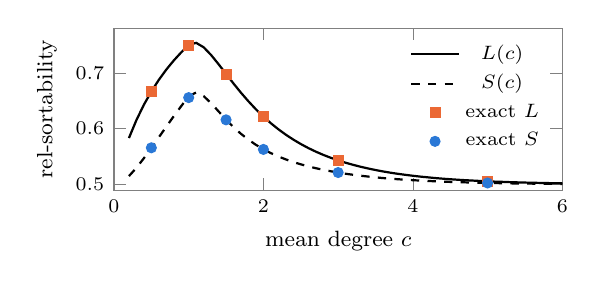
\begin{tikzpicture}
\begin{axis}[width=0.6\textwidth, height=0.3\textwidth, xmin=0, xmax=6, ymin=0.49, ymax=0.78,
  xlabel={mean degree $c$}, ylabel={rel-sortability},
  tick label style={font=\scriptsize}, label style={font=\footnotesize},
  legend style={font=\scriptsize, draw=none, fill=none, at={(0.98,0.97)}, anchor=north east},
  axis line style={gray}, tick style={gray}]
\addplot[thick,black] coordinates {(0.2,0.5833) (0.3,0.6154) (0.4,0.6429) (0.5,0.6667) (0.6,0.6875) (0.7,0.7059) (0.8,0.7222) (0.9,0.7368) (1.0,0.7500) (1.1,0.7538) (1.2,0.7459) (1.3,0.7320) (1.4,0.7155) (1.5,0.6981) (1.6,0.6809) (1.7,0.6644) (1.8,0.6490) (1.9,0.6347) (2.0,0.6217) (2.1,0.6098) (2.2,0.5990) (2.3,0.5893) (2.4,0.5805) (2.5,0.5726) (2.6,0.5654) (2.7,0.5590) (2.8,0.5532) (2.9,0.5480) (3.0,0.5433) (3.1,0.5391) (3.2,0.5353) (3.3,0.5319) (3.4,0.5288) (3.5,0.5260) (3.6,0.5235) (3.7,0.5212) (3.8,0.5192) (3.9,0.5174) (4.0,0.5157) (4.1,0.5142) (4.2,0.5129) (4.3,0.5116) (4.4,0.5105) (4.5,0.5095) (4.6,0.5086) (4.7,0.5078) (4.8,0.5071) (4.9,0.5064) (5.0,0.5058) (5.1,0.5052) (5.2,0.5048) (5.3,0.5043) (5.4,0.5039) (5.5,0.5035) (5.6,0.5032) (5.7,0.5029) (5.8,0.5026) (5.9,0.5024) (6.0,0.5022)};
\addplot[thick,black,dashed] coordinates {(0.2,0.5151) (0.3,0.5299) (0.4,0.5471) (0.5,0.5656) (0.6,0.5846) (0.7,0.6036) (0.8,0.6224) (0.9,0.6405) (1.0,0.6580) (1.1,0.6649) (1.2,0.6584) (1.3,0.6457) (1.4,0.6310) (1.5,0.6163) (1.6,0.6028) (1.7,0.5908) (1.8,0.5803) (1.9,0.5711) (2.0,0.5632) (2.1,0.5563) (2.2,0.5503) (2.3,0.5450) (2.4,0.5403) (2.5,0.5362) (2.6,0.5325) (2.7,0.5293) (2.8,0.5264) (2.9,0.5238) (3.0,0.5214) (3.1,0.5193) (3.2,0.5175) (3.3,0.5158) (3.4,0.5143) (3.5,0.5129) (3.6,0.5116) (3.7,0.5105) (3.8,0.5095) (3.9,0.5086) (4.0,0.5078) (4.1,0.5071) (4.2,0.5064) (4.3,0.5058) (4.4,0.5052) (4.5,0.5047) (4.6,0.5043) (4.7,0.5039) (4.8,0.5035) (4.9,0.5032) (5.0,0.5029) (5.1,0.5026) (5.2,0.5024) (5.3,0.5021) (5.4,0.5019) (5.5,0.5018) (5.6,0.5016) (5.7,0.5014) (5.8,0.5013) (5.9,0.5012) (6.0,0.5011)};

\addplot[only marks, mark=square*, mark size=1.8pt, color={rgb,255:red,235;green,104;blue,52}]
  coordinates {(0.5,0.6666) (1,0.7486) (1.5,0.6975) (2,0.6214) (3,0.5434) (5,0.5059)};
\addplot[only marks, mark=*, mark size=1.8pt, color={rgb,255:red,42;green,120;blue,214}]
  coordinates {(0.5,0.5658) (1,0.6557) (1.5,0.6159) (2,0.5629) (3,0.5215) (5,0.5028)};
\legend{$L(c)$,$S(c)$,exact $L$,exact $S$}
\end{axis}
\end{tikzpicture}
\caption{\cref{prop:er} (lines) against exact computation on seeded graphs
($p=2\cdot10^4$ to $10^5$; points, means over seeds). The standard deviations
over seeds are at most $0.0022$ (\cref{app:er}).}
\label{fig:er}
\end{figure}



\textbf{In-forests (proved identities).} Let the non-loop part be an in-forest
with $m$ edges and $n_1$ nodes with exactly one parent. By
\cref{cor:iff,cor:statiff},
$L=\tfrac12+\frac{m}{2(m+p)}$, $S=\tfrac12+\frac{m-n_1}{2(m+p)}$,
$L-S=\frac{n_1}{2(m+p)}$ (the last checked to machine precision on $18$ random
forests). For a sequence of in-forests with parent-count distribution $\pi$ and
mean $\mu$: $L\to\tfrac12+\frac\mu{2(1+\mu)}$ and
$S\to\tfrac12+\frac{\mu-\pi_1}{2(1+\mu)}$. Exact computation at $p=20{,}000$
(6 seeds each): uniform recursive in-tree ($\pi_1=1/4$, $S\to11/16=0.6875$,
measured $0.68739\pm0.00026$); preferential attachment (measured $\pi_1=0.1656$,
$S=0.70859\pm0.00028$); uniform random labelled tree rooted and oriented to the
root (Poisson(1) parents, $\pi_1\to e^{-1}$, $S\to\tfrac12+(1-e^{-1})/4=0.65803$,
measured $0.65783\pm0.00020$). In all three $L=0.74999$.

\textbf{Directed ER: summary.} $G(p,c/p)$, $m/p\to c$. The finite limit needs
the fraction of non-loop edges inside an SCC ($\to x^2$, the two endpoints lie in
the giant SCC iff the ancestor tree of $i$ and the descendant tree of $j$ are
infinite); the stationary value needs the fraction of up-edges
($\to F_\uparrow$). Both are proved in \cref{app:erproof} below. Large $c$:
$1-x\sim e^{-c}$, $L-\tfrac12\sim e^{-c}$, $S-\tfrac12\sim e^{-c}/2$.

\textbf{Layered DAG (sketch; $L$ proved given edge concentration).} $M$ layers of
width $w$, each node of layer $l+1$ receiving an edge from each node of layer $l$
with probability $c/w$; as $w\to\infty$ with $\mu=c(M-1)/M$,
$L\to\tfrac12+\frac\mu{2(1+\mu)}$ and
$S\to\tfrac12+\frac{\mu(1-e^{-c})}{2(1+\mu)}$. For fixed $w$ and deep $M$ the
stationary value falls below this (observed $0.7824$ against $0.7878$ at
$w=50$, $M=400$, $c=2$); this correction is not derived.

\begin{table}[h]
\caption{Exact computation (means $\pm$ s.d.\ over seeds; SCCs by scipy and source sets by bitsets) against the limits of \cref{prop:er}, proved in \cref{app:erproof}.}
\label{tab:er}
\centering
\begin{tabular}{rrcccc}
\toprule
$c$ & $p$ & $L$ exact & $L$ formula & $S$ exact & $S$ formula \\
\midrule
0.5 & 20000 & $0.6666\pm0.0011$ & $0.6667$ & $0.5658\pm0.0014$ & $0.5656$ \\
1.0 & 20000 & $0.7486\pm0.0008$ & $0.7500$ & $0.6557\pm0.0013$ & $0.6580$ \\
1.5 & 50000 & $0.6975\pm0.0020$ & $0.6981$ & $0.6159\pm0.0018$ & $0.6163$ \\
2.0 & 50000 & $0.6214\pm0.0022$ & $0.6217$ & $0.5629\pm0.0014$ & $0.5632$ \\
3.0 & 100000 & $0.5434\pm0.0010$ & $0.5433$ & $0.5215\pm0.0006$ & $0.5214$ \\
5.0 & 20000 & $0.5059\pm0.0005$ & $0.5058$ & $0.5028\pm0.0003$ & $0.5029$ \\
\bottomrule
\end{tabular}
\end{table}
At the critical point $c=1$, $S$ converges slowly in $p$: $0.65574\pm0.00126$ ($p=2\cdot10^4$, 6 seeds),
$0.65784\pm0.00043$ ($2\cdot10^5$, 6 seeds) and $0.65796$ ($10^6$, 1 seed) against $0.65803$, like $L$
($0.74857$, $0.74972$, $0.74989$ against $0.75$).

$L$ at $c=1$ converges as $p$ grows: $0.7466$ ($p=2000$), $0.7486$ ($2\cdot10^4$),
$0.74976$ ($2\cdot10^5$), $0.74992$ ($10^6$); at $c=2$, $0.62162\pm0.00023$ at
$p=10^6$ against $0.62170$. The giant-SCC fraction matches $x^2$ ($0.6353$ against
$0.6349$ at $c=2$). The second fixed point matters: with $d=1$ the formula would
give $S=0.6312$, $0.5766$, $0.5246$ at $c=1.5,2,3$, outside the error bars,
whereas the fixed points $d=0.485$, $0.221$, $0.061$ give $0.6163$, $0.5632$,
$0.5214$. Further exact rows: $c=1.5$, $p=10^5$, 32 graphs, $L=0.69819\pm0.00024$
(formula $0.69810$); $c=2$, $p=3.2\cdot10^5$, $L=0.62170\pm0.00012$ ($0.62170$).
The Barak--Erd\H{o}s phase-transition paper cited by \citet{reisach2026topological}
concerns monotone-path reachability at the dense scale $\log n/n$ and is not
used here.

\subsection{Directed Erd\H{o}s--R\'enyi summary graphs: full proof of \cref{prop:er}}
\label{app:erproof}

\textbf{Status.} Everything in this subsection is proved on paper. The only
inputs used without proof are textbook facts (F1)--(F3) below, checked against
the author's online version of \citet{hofstad2016random} (theorem numbers are
those of that version and may differ in print). Lemma~\ref{lem:er-local} is the
standard local-coupling argument for sparse random graphs and is written
concisely. The deterministic witness lemmas are machine-checked; no
probabilistic step is. No human probabilist has yet checked this subsection
(see the AI-use statement).

\textbf{Limits and their order.} For a fixed summary graph, \cref{thm:limit}
gives $\lim_{T\to\infty}\srho(\GT)=L(\GS)=\tfrac12+|\Ex|/(2|\Es|)$, and
\cref{thm:stat} gives $\srho^W=\tfrac12+|\Eu|/(2|\Es|)$ for every $T$. For
$\GS\sim D(p,c/p)$ we take the limit $T\to\infty$ at fixed $p$ first (this
defines $L(\GS)$) and then let $p\to\infty$; for the stationary value no
$T$-limit is needed. The regime of fixed $T$ with $p\to\infty$ is not covered
(the bound of \cref{thm:limit} is vacuous for $T\le p$).

\textbf{Model and notation.} $D(p,c/p)$: each ordered pair $(i,j)$, $i\ne j$,
is a non-loop edge independently with probability $q=c/p$, and every node has
a self-loop (loops change neither reachability nor $\Src$). $m$ is the number of
non-loop edges, $|\Es|=p+m$, $N$ the number of non-loop edges inside an SCC, so
$|\Ex|=m-N$. $\mathrm{out}(v)$, $\mathrm{in}(v)$ are the sets of nodes
reachable from $v$, resp.\ reaching $v$ ($v$ included), $T^{\mathrm{out}}_v$,
$T^{\mathrm{in}}_v$ their sizes; $v\leadsto w$ means $w\in\mathrm{out}(v)$.
$x=x(c)$ is the largest solution of $x=1-e^{-cx}$ (the survival probability of
a Poisson$(c)$ Galton--Watson tree), $\theta_K=\theta_K(c)$ the probability that
its total progeny is at least $K$ ($\theta_K\downarrow x$), and $d$ the smallest
fixed point in $[0,1]$ of $f(d)=1+e^{-c}-e^{-c(1-x)d}$. A node is
\emph{in-isolated} if it has no non-loop parent. $\mathcal G$ denotes the
\emph{edge-rooted Poisson tree}: an edge $(i,j)$; $i$ has Poisson$(c)$ parents
and Poisson$(c)$ further children, $j$ Poisson$(c)$ further parents and
Poisson$(c)$ children; every other node has Poisson$(c)$ parents and
Poisson$(c)$ children besides the edge through which it was reached; all
independent.

\textbf{Textbook facts.} (F1) Poisson coupling \citep[Thm.~2.10]{hofstad2016random}:
$d_{\mathrm{TV}}(\mathrm{Bin}(n,q),\mathrm{Poi}(c))\le nq^2+|nq-c|$.
(F2) Chernoff: for a sum $X$ of independent Bernoulli variables with mean
$\mu$ and $\delta\in(0,1)$, $P(X\le(1-\delta)\mu)\le e^{-\delta^2\mu/2}$. (From
$Ee^{-tX}\le\exp(\mu(e^{-t}-1))$ with $t=-\log(1-\delta)$, Markov's inequality,
and $(1-\delta)\log(1-\delta)\ge-\delta+\delta^2/2$; the upper-tail version
$P(X\ge\mu+s)\le e^{-s}$ for $s\ge e^2\mu$ follows in the same way.)
(F3) Galton--Watson facts \citep[Thms.~3.1, 3.16]{hofstad2016random}: the
extinction probability is the smallest root of $\eta=e^{c(\eta-1)}$, so the
survival probability is $x(c)$, positive iff $c>1$.

\textbf{Deterministic lemmas} (machine-checked, \lname{ErLemmas.lean}; no loop
hypothesis). A node $z$ is a \emph{source node} if every ancestor of $z$ is
reachable from $z$. By \cref{thm:stat}, $(i,j)\in\Eu$ iff some source node
reaches $j$ but not $i$.
\begin{itemize}
\item[(W1)] If $(i,j)\in\Eu$, there are $k\notin\{i,j\}$ with $k\to j$ and a
source node $z$ with $z\leadsto k$, $z\not\leadsto i$ (\lname{upEdge_witness}).
\item[(W2)] If $i\to j$, $k\to j$, and a source node reaches $k$ but not $i$,
then $(i,j)\in\Eu$ (\lname{mem_upEdges_of_witness}).
\item[(W3)] If $i\to j$, $k\to j$ and $\mathrm{in}(k)\cap\mathrm{in}(i)=\emptyset$,
then $(i,j)\in\Eu$ (\lname{mem_upEdges_of_disjoint_anc}).
\item[(W5)] A non-loop edge $(i,j)$ lies inside an SCC iff $j\leadsto i$. The
event $\{j\leadsto i\}$ and the set $\mathrm{out}(j)$ do not change when the
edge $(i,j)$ is added or removed (a simple path from $j$ to $i$ does not use
it). (Trivial; not formalised.)
\end{itemize}

\textbf{Explorations and forced edges.} Forward exploration of $\mathrm{out}(v)$
keeps explored, active and unseen sets $X_t,A_t,U_t$, $a_t=|A_t|$,
$\mathrm{disc}_t=t+a_t$, $X_0=\emptyset$, $A_0=\{v\}$. Step $t+1$ takes the
oldest active node $w$, reveals the pairs $(w,u)$, $u\in U_t$, and makes the
$\xi_{t+1}$ heads of present pairs active; it stops at $T=T^{\mathrm{out}}_v$.
Backward exploration of $\mathrm{in}(v)$ reveals the pairs $(u,w)$ instead.
Let $F$ be a set of at most three ordered pairs and $G^F$ the graph in which the
pairs of $F$ are present and all other pairs are independent Be$(q)$.
\emph{Bookkeeping.} In a forward exploration a pair is revealed only when its
tail is explored, and each node is explored once, so each pair is revealed at
most once; the pairs revealed at step $t+1$ are disjoint from those revealed
before and from all pairs whose tail is not in $X_{t+1}$. Hence, conditionally
on the history $\mathcal H_t$, the non-forced pairs revealed at step $t+1$ are
independent Be$(q)$, and
$\xi_{t+1}=\#\{u\in U_t:(w,u)\in F\}+\mathrm{Bin}(|U_t|-f_w,q)$ with
$f_w\le3$ the number of forced pairs from $w$ into $U_t$. Thus, given
$\mathcal H_t$, $\xi_{t+1}$ stochastically dominates $\mathrm{Bin}(|U_t|-3,q)$
and is dominated by $3+\mathrm{Bin}(p,q)$. The same holds for backward
explorations (with heads in place of tails), and, by the same argument, for a
backward exploration run after a forward one, conditionally on the forward
history, as long as it never discovers a node that the forward exploration
discovered (only pairs with tail outside $X_f$ and head explored backward are
revealed, and none of them was revealed forward).

Fix $c>1$ and $\varepsilon\in(0,1/5)$ with $\beta=c(1-4\varepsilon)>1$; put
$n'=\lceil(1-4\varepsilon)p\rceil$, $\kappa=(\beta-1)^2/(8\beta)$,
$\delta=(\beta-1)\varepsilon/(\beta+1)$, $t_0=C_3\log p$ with $C_3\kappa\ge8$.
Call an exploration \emph{admissible} if, conditionally on its history, every
offspring count $\xi_{t+1}$ taken while $\mathrm{disc}_t<\varepsilon p$
dominates $\mathrm{Bin}(n',q)$ and every offspring count is dominated by
$3+\mathrm{Bin}(p,q)$. By the bookkeeping, forward and backward explorations in
$G^F$ are admissible for large $p$ (since $|U_t|-3>(1-\varepsilon)p-3\ge n'$),
and so is the backward exploration of Lemma~\ref{lem:er-l2} below.

\begin{lemma}[dichotomy]\label{lem:er-l1}
There is $C$ (depending on $c,\varepsilon$) such that for large $p$ every
admissible exploration with final size $T$ satisfies
(a) $P(K\le T<\varepsilon p)\le Ce^{-\kappa K}$ for all $K\ge1$;
(b) $P\big(T\ge t_0$ and [$\mathrm{disc}_t<\varepsilon p$ for all $t$, or
$a_\tau<\delta p$ at $\tau=\min\{t:\mathrm{disc}_t\ge\varepsilon p\}$]$\big)\le Cp^{-8}$.
Consequently, with probability at least $1-Cp^{-7}$, every node $v$ of $G$ has, in
both directions, $T_v<t_0$ or ($T_v\ge\varepsilon p$ and $a_\tau\ge\delta p$).
\end{lemma}
\begin{proof}
Let $\xi'_t$ be independent $\mathrm{Bin}(n',q)$ variables coupled so that
$\xi_t\ge\xi'_t$ for $t\le\tau$ (admissibility; after $\tau$ or after the
exploration stops, $\xi'_t$ uses external randomness), and
$W_t=1+\sum_{s\le t}(\xi'_s-1)$. By induction $a_t\ge W_t$ for
$t\le\min(T,\tau)$. Since $tn'q\ge t\beta$ and
$(\beta+1)/2=(1-\frac{\beta-1}{2\beta})\beta$, (F2) gives
$P(W_t\le(\beta-1)t/2)\le P(\mathrm{Bin}(tn',q)\le t(\beta+1)/2)\le e^{-\kappa t}$,
so $\mathrm{Bad}(t_1)=\{\exists t\ge t_1:W_t\le(\beta-1)t/2\}$ has probability at
most $e^{-\kappa t_1}/(1-e^{-\kappa})$.
(a) If $T<\varepsilon p$ then $\tau=\infty$, so $0=a_T\ge W_T$, which is
$\mathrm{Bad}(K)$ when $T\ge K$.
(b) On $\mathrm{Bad}(t_0)^c$ with $T\ge t_0$: for $t_0\le t\le\min(T,\tau)$,
$a_t\ge W_t>0$, so the exploration cannot stop before $\tau$, hence
$\tau<\infty$. At $\tau$, $a_\tau+\tau\ge\varepsilon p$, and if $\tau\ge t_0$
also $a_\tau>(\beta-1)\tau/2$; minimising $\max((\beta-1)\tau/2,\varepsilon p-\tau)$
over $\tau$ gives $a_\tau\ge\delta p$; if $\tau<t_0$, $a_\tau\ge\varepsilon p-t_0\ge\delta p$.
$e^{-\kappa t_0}\le p^{-8}$. The consequence is a union bound over $p$ nodes and
two directions.
\end{proof}

\begin{lemma}[large out-sets reach large in-sets]\label{lem:er-l2}
With probability at least $1-Cp^{-5}$: for all $v,w$, $T^{\mathrm{out}}_v\ge t_0$
and $T^{\mathrm{in}}_w\ge t_0$ imply $v\leadsto w$.
\end{lemma}
\begin{proof}
Fix $(v,w)$. Explore $\mathrm{out}(v)$ forward up to $\tau_f$ (history $\mathcal H_f$,
discovered set $R_f=X_f\cup A_f$). Since every $\xi$ is dominated by
$3+\mathrm{Bin}(p,q)$, $P(\max_t\xi_t\ge\varepsilon p)\le e^{-\varepsilon p}$ for
large $p$ (F2, upper tail), so $|R_f|\le2\varepsilon p$ except on that event.
Then explore $\mathrm{in}(w)$ backward, stopping at $\tau_b$ or when a node of
$R_f\subseteq\mathrm{out}(v)$ is discovered; in the latter case $v\leadsto w$.
Otherwise the backward exploration is the true exploration of $\mathrm{in}(w)$,
its unseen set has at least $p-2\varepsilon p-\varepsilon p-3\ge n'$ usable
nodes while $\mathrm{disc}<\varepsilon p$, and by the bookkeeping it is admissible
conditionally on $\mathcal H_f$. By Lemma~\ref{lem:er-l1}(b) for both
explorations, outside probability $2Cp^{-8}$: if $T^{\mathrm{out}}_v,T^{\mathrm{in}}_w\ge t_0$
and no connection occurred, then $|A_f|,|A_b|\ge\delta p$. $A_f$ and $A_b$ are
disjoint, and every pair $(a,a')\in A_f\times A_b$ is unrevealed (its tail is not
in $X_f$, its head not in $X_b$), so given both histories these pairs are
independent Be$(q)$ (or forced present): $P(\text{no edge }A_f\to A_b)\le(1-q)^{\delta^2p^2-3}\le e^{-c\delta^2p/2}$.
An edge $a\to a'$ gives $v\leadsto a\to a'\leadsto w$. Union bound over $p^2$
pairs.
\end{proof}

Let $\Omega$ be the intersection of the events of Lemma~\ref{lem:er-l1}
(consequence) and Lemma~\ref{lem:er-l2}, $P(\Omega^c)\le Cp^{-5}$. Put
$\mathcal S=\{v:T^{\mathrm{out}}_v\ge t_0\}$, $\mathcal T=\{v:T^{\mathrm{in}}_v\ge t_0\}$.

\begin{corollary}[structure]\label{cor:er-struct}
On $\Omega$: $\mathcal S\times\mathcal T$ is contained in the reachability
relation; every SCC other than the one containing $\mathcal S\cap\mathcal T$ has
fewer than $t_0$ nodes; if $|\mathcal S\cap\mathcal T|\ge t_0$, this SCC equals
$\mathcal S\cap\mathcal T$.
\end{corollary}
\begin{proof}
The first claim is Lemma~\ref{lem:er-l2}. A node $u\notin\mathcal S\cap\mathcal T$
has $T^{\mathrm{out}}_u<t_0$ or $T^{\mathrm{in}}_u<t_0$, and its SCC lies in
$\mathrm{out}(u)\cap\mathrm{in}(u)$. If $u$ were in the SCC of
$\mathcal S\cap\mathcal T$, that SCC (of size $\ge t_0$) would lie in
$\mathrm{out}(u)\cap\mathrm{in}(u)$, a contradiction.
\end{proof}
(This re-proves the part of the Karp--{\L}uczak structure theorem we need; the
statement is recorded in the introduction of \citealp{dovgal2020birth}.)

\begin{lemma}[local concentration; standard coupling]\label{lem:er-local}
Fix $R$ and a function $\varphi$ of the isomorphism class of the radius-$R$
neighbourhood $B_R(e)$ of a non-loop edge $e$ (all edges incident to nodes at
undirected distance $<R$ from $e$, rooted at the oriented edge $e$), and let
$\Phi_p=p^{-1}\sum_e\varphi(B_R(e))$, the sum over non-loop edges.
(a) If $\varphi$ is bounded, $E\Phi_p\to cE_{\mathcal G}\varphi$ and
$\mathrm{Var}\,\Phi_p\to0$; the same holds for node-rooted functionals with the
node-rooted Poisson tree.
(b) If $\varphi\ge0$ and $\varphi(B_R(e))\le\mathrm{indeg}(j)$ for $e=(i,j)$, then
$\limsup_pE\Phi_p\le cE_{\mathcal G}[\min(\varphi,M)]+C/M$ for every $M$, with $C$
not depending on $p$ or $M$.
\end{lemma}
\begin{proof}
(a) First moment:
$E\sum_e\varphi(B_R(e))=\sum_{(i,j)}q\,E[\varphi(B_R((i,j);G\cup\{(i,j)\}))]$.
Explore the undirected neighbourhood of $(i,j)$ breadth first, revealing for
each explored node $w$ all pairs $(w,u)$ and $(u,w)$. On $\{|B_R|\le M\}$, each
explored node has $\mathrm{Bin}(|U|,q)$ new children and $\mathrm{Bin}(|U|,q)$
new parents among the unseen nodes, $|U|\ge p-M$, which (F1) couples with
Poisson$(c)$ up to an error $\le Mq^2p+cM/p$ per count, and the pairs between
already seen nodes are present with total probability $\le M^2q$. So the
truncated ball is within $C(M,R)/p$ in total variation of the truncated
$\mathcal G$. Tightness: each exploration step is dominated by
$\mathrm{Bin}(2p,q)$ (resp.\ Poisson$(2c)$), so $E|B_R|\le(1+2c+o(1))^R$ and
$P(|B_R|>M)\le C^R/M$ uniformly in $p$; let $p\to\infty$, then $M\to\infty$.
Second moment: $E\Phi_p^2=p^{-2}\big[\sum_e+\sum_{e,f\text{ sharing a node}}+\sum_{e,f\text{ node-disjoint}}\big]$.
The first two sums are $O(p)$ since $E\sum_vd(v)^2=O(p)$. For node-disjoint
$e,f$, explore both balls jointly in $G\cup\{e,f\}$: on $\{$both sizes $\le M\}$
they are disjoint and non-adjacent except with probability $\le C(M,R)/p$, and
then the two explorations are coupled with independent copies of $\mathcal G$.
Hence $p^{-2}\sum_{\text{disjoint}}\to(cE_{\mathcal G}\varphi)^2$ and
$\mathrm{Var}\,\Phi_p\to0$.
(b) Apply (a) to $\min(\varphi,M)$ and bound the rest by
$E\sum_{(i,j)}\mathrm{indeg}(j)\mathbf 1[\mathrm{indeg}(j)>M]=E\sum_j\mathrm{indeg}(j)^2\mathbf 1[\mathrm{indeg}(j)>M]\le p\,E[D^3]/M$,
$D\sim\mathrm{Bin}(p-1,q)$, and $E[D^3]\le c^3+3c^2+c$ for all $p$ (uniform
integrability).
\end{proof}

\textbf{Local functionals.} All of the following are functions of $B_{2K+1}(e)$
(a breadth-first search of the first $K$ nodes of a set stays within distance
$K-1$), are invariant under isomorphism, and count all qualifying nodes, so no
labelling enters.
$A^K_e=\mathbf 1[T^{\mathrm{out}}_j\ge K,\ T^{\mathrm{in}}_i\ge K]$, with
$E_{\mathcal G}A^K=\theta_K^2$ (the descendant tree of $j$ and the ancestor tree
of $i$ are independent Poisson Galton--Watson trees).
$\Psi_K(e)=\mathrm{cl}_1\vee\mathrm{cl}_2$, with
$\mathrm{cl}_1=[T^{\mathrm{in}}_i<K$ and $j$ has a parent $k\notin\{i,j\}]$ and
$\mathrm{cl}_2=[$some in-isolated $s$ has $T^{\mathrm{out}}_s<K$, $j\in\mathrm{out}(s)$, $i\notin\mathrm{out}(s)]$.
$\varphi^{\beta}_K(e)=\#\{k\notin\{i,j\}:k\to j,\ T^{\mathrm{in}}_k<K,\ T^{\mathrm{in}}_i<K,\ \mathrm{in}(k)\cap\mathrm{in}(i)\ne\emptyset\}\le\mathrm{indeg}(j)$,
with $E_{\mathcal G}\min(\varphi^\beta_K,M)=0$ (in $\mathcal G$ the ancestor trees
of $i$ and of another parent of $j$ are disjoint).

\begin{proposition}[$L$, $c>1$]\label{prop:er-N}
For $c>1$, $N/p\to cx^2$ in $L^1$ and in probability.
\end{proposition}
\begin{proof}
By (W5), $N=\sum_eZ_e$ with $Z_e=\mathbf 1[j\leadsto i]$; compare with
$\tilde N_K=\sum_eA^K_e$.
(i) $Z=1,A=0$: $j\leadsto i$ and ($T^{\mathrm{out}}_j<K$ or $T^{\mathrm{in}}_i<K$).
By (W5) these events do not depend on the presence of $e$, so the expected
number of such edges is $p(p-1)q\,P(i\in\mathrm{out}(j),T^{\mathrm{out}}_j<K)$ plus
the same with $\mathrm{in}(i)$, and by exchangeability of the $p-1$ nodes other
than $j$, $P(i\in\mathrm{out}(j),T^{\mathrm{out}}_j<K)=E[(T^{\mathrm{out}}_j-1)\mathbf 1(T^{\mathrm{out}}_j<K)]/(p-1)\le K/(p-1)$.
Total $\le2cK$.
(ii) $Z=0,A=1$: on $\Omega$, $T^{\mathrm{out}}_j\ge t_0$ and $T^{\mathrm{in}}_i\ge t_0$
would give $j\leadsto i$, so $T^{\mathrm{out}}_j$ or $T^{\mathrm{in}}_i$ lies in
$[K,t_0)\subseteq[K,\varepsilon p)$. The expected number of such edges is at
most $\sum_{(i,j)}q\,P_{G^{\{e\}}}(\cdot)\le cp\cdot2Ce^{-\kappa K}$ by
Lemma~\ref{lem:er-l1}(a) in $G^{\{e\}}$; on $\Omega^c$ the count is at most $m$
and $E[m\mathbf 1_{\Omega^c}]\le(Em^2)^{1/2}P(\Omega^c)^{1/2}=O(p\cdot p^{-5/2})$.
So $E|N-\tilde N_K|\le2cK+2cCpe^{-\kappa K}+o(1)$. By
Lemma~\ref{lem:er-local}(a), $\tilde N_K/p\to c\theta_K^2$ in $L^2$; hence
$\limsup_pE|N/p-cx^2|\le2cCe^{-\kappa K}+c|\theta_K^2-x^2|\to0$ as $K\to\infty$.
\end{proof}
The same argument for the node functional $\mathbf 1[T^{\mathrm{out}}_v\ge K,T^{\mathrm{in}}_v\ge K]$
gives $|\mathcal S\cap\mathcal T|/p\to x^2$, so by \cref{cor:er-struct} the giant
SCC has $(x^2+o_P(1))p$ nodes and all other SCCs fewer than $C_3\log p$, w.h.p.

\begin{proposition}[the tree computation]\label{prop:er-tree}
In $\mathcal G$, with $\Psi_\infty$ defined by $T^{\mathrm{in}}_i<\infty$ and
$T^{\mathrm{out}}_s<\infty$, $E_{\mathcal G}\Psi_K\uparrow P_{\mathcal G}(\Psi_\infty)=F_\uparrow$
as $K\to\infty$.
\end{proposition}
\begin{proof}
Both clauses increase in $K$ to their $K=\infty$ versions (monotone convergence).
Let $A(i)$ be the event that the ancestor tree of $i$ is infinite and $D(j)$ that
the descendant tree of $j$ is infinite (probability $x$ each, independent). The
other parents of $j$ are Poisson$(c)$ many.
(1) Not $A(i)$: $\Psi_\infty$ holds iff $j$ has another parent. Clause 1 needs
exactly that; clause 2 needs it too, since a path from $s$ to $j$ ends with an
edge $k\to j$ and $k=i$ would put $i$ into $\mathrm{out}(s)$. Probability
$(1-x)(1-e^{-c})$.
(2) $A(i)$: clause 1 fails. Clause 2 needs (a) not $D(j)$, since
$\mathrm{out}(s)$ contains the descendant tree of $j$ (probability $1-x$), and
(b) another parent $k$ of $j$ and a chain $k=u_0\leftarrow u_1\leftarrow\dots\leftarrow u_r=s$
ending at an in-isolated $s$, in which every $u_t$ has only finite descendant
trees below its children other than $u_{t-1}$ ($u_{-1}=j$); such an $s$ does not
reach $i$, because paths into $i$ stay in the ancestor tree of $i$. The
probability that all other children of a node have finite descendant trees is
$E[(1-x)^{\mathrm{Poi}(c)}]=e^{-cx}=1-x$. Let $Q(v)$ be the event that $v$ is
in-isolated or some parent $u$ of $v$ has all other children finite and $Q(u)$
holds, and $d^*=P(Q)$. Parents are Poisson$(c)$ many and each is \emph{good}
(other children finite and $Q$) independently with probability $(1-x)d^*$, so by
Poisson thinning $d^*=e^{-c}+1-e^{-c(1-x)d^*}=f(d^*)$. $Q$ is the increasing
union of its depth-$n$ truncations $Q_n$, with $P(Q_0)=e^{-c}=f(0)$ and
$P(Q_{n+1})=f(P(Q_n))$; as $f$ is increasing and continuous, $P(Q_n)=f^{n+1}(0)$
increases to the smallest fixed point $d$ of $f$ (if $d'$ is a fixed point,
$f^n(0)\le f^n(d')=d'$). So $d^*=d$. The number of good other parents of $j$ is
Poisson$(c(1-x)d)$, so (b) has probability $1-e^{-c(1-x)d}$, independently of
$A(i)$ and $D(j)$. Adding (1) and (2) gives $F_\uparrow$.
\end{proof}
(An independent Monte Carlo of the event itself, not of the closed form, gives
$0.38756\pm0.00077$ against $0.38773$ at $c=1.5$ and $0.19049\pm0.00062$ against
$0.18962$ at $c=2$.)

\begin{proposition}[reduction of $\Eu$ to $\Psi_K$, $c>1$]\label{prop:er-red}
$E\sum_e|\mathbf 1[e\in\Eu]-\Psi_K(e)|\le(\delta_1(K)+o(1))p$ with
$\delta_1(K)=C(c^2+K^2)e^{-\kappa K}+o_K(1)$, where $o_K(1)\to0$ as $K\to\infty$
and $C$ does not depend on $K$ or $p$.
\end{proposition}
\begin{proof}
Let $e=(i,j)$ be a non-loop edge. \emph{Clause 2 never errs}: an in-isolated $s$
is a source node, so $j\in\mathrm{out}(s)$, $i\notin\mathrm{out}(s)$ give
$e\in\Eu$. \emph{Case I: $T^{\mathrm{in}}_i<K$.} (I-a) If $e\in\Eu$, (W1) gives
another parent of $j$, so clause 1 holds: no error. (I-b) Clause 1 holds and
$e\notin\Eu$. Then
$\mathbf 1[\text{I-b}]\le\sum_{k\notin\{i,j\}}\mathbf 1[e,(k,j)\text{ present},\ T^{\mathrm{in}}_i<K,\ e\notin\Eu]$
(a union over \emph{all} other parents; no parent is singled out). Fix the
triple $(i,j,k)$ and force $F=\{(i,j),(k,j)\}$. By (W3), $e\notin\Eu$ forces
$\mathrm{in}(k)\cap\mathrm{in}(i)\ne\emptyset$, and by (W2) every source node
reaching $k$ reaches $i$. Split on $T^{\mathrm{in}}_k$:
($\alpha_1$) $K\le T^{\mathrm{in}}_k<\varepsilon p$: probability $\le Ce^{-\kappa K}$
(Lemma~\ref{lem:er-l1}(a), backward, in $G^F$).
($\alpha_2$) $T^{\mathrm{in}}_k\ge\varepsilon p$: the backward exploration of
$\mathrm{in}(k)$ explores at least $\varepsilon p/2$ nodes. When a node $y\ne j$ is
explored, the pairs $(u,y)$ with $u$ unseen are revealed (all absent with
conditional probability $\ge(1-q)^p$), and the pairs $(u,y)$ with $u$ already
seen are never revealed by this exploration and are independent of it and of
each other (distinct heads); so, given the history, $y$ is in-isolated with
probability $\ge(1-q)^p\ge e^{-c}/2$, and the number of in-isolated nodes among
the first $\varepsilon p/2$ explored nodes dominates
$\mathrm{Bin}(\varepsilon p/2-1,e^{-c}/2)$. By (F2) at least $K$ of them are
in-isolated except with probability $e^{-\Omega(p)}$. Each in-isolated node of
$\mathrm{in}(k)$ is a source node reaching $k$, hence reaches $i$, so lies in
$\mathrm{in}(i)$; but $|\mathrm{in}(i)|<K$. So ($\alpha_2$) has probability
$e^{-\Omega(p)}$.
($\beta$) $T^{\mathrm{in}}_k<K$ and $\mathrm{in}(k)\cap\mathrm{in}(i)\ne\emptyset$.
Summed over $k$ this is $\varphi^\beta_K(e)$.
The number of triples is $p^3$ and each has both pairs present with probability
$q^2$, so cases ($\alpha_1$), ($\alpha_2$) contribute at most
$c^2p(Ce^{-\kappa K}+e^{-\Omega(p)})$; case ($\beta$) contributes
$E\sum_e\varphi^\beta_K(e)\le(C/M+o(1))p$ for every $M$ by
Lemma~\ref{lem:er-local}(b), i.e.\ $o(p)$.
\emph{Case II: $T^{\mathrm{in}}_i\ge K$.} Clause 1 fails.
(II-0) $K\le T^{\mathrm{in}}_i<\varepsilon p$: at most $cpCe^{-\kappa K}$ such
edges in expectation (Lemma~\ref{lem:er-l1}(a) in $G^{\{e\}}$).
(II-1) $T^{\mathrm{in}}_i\ge\varepsilon p$, so $i\in\mathcal T$. Work on
$\Omega'=\Omega\cap\{\max_v\mathrm{indeg}(v)\le C\log p\}$; $P(\Omega'^c)\le Cp^{-2}$,
and the edges counted on $\Omega'^c$ contribute at most
$E[m\mathbf 1_{\Omega'^c}]\le(Em^2)^{1/2}P(\Omega'^c)^{1/2}=O(1)$. An error here is
an edge $e\in\Eu$ with $\Psi_K(e)=0$. Take a witness source node $z$ of (W1),
in a source SCC $\sigma$. On $\Omega$, $z\in\mathcal S$ would give $z\leadsto i$
(Lemma~\ref{lem:er-l2}), so $T^{\mathrm{out}}_z<t_0$.
(A) $\sigma=\{z\}$ (i.e.\ $z$ in-isolated) and $T^{\mathrm{out}}_z<K$: clause 2
holds with $s=z$; no error.
(B1) $z$ in-isolated and $K\le T^{\mathrm{out}}_z<t_0$. The number of such edges
is at most $\sum_z\mathbf 1[K\le T^{\mathrm{out}}_z<t_0]\sum_{j\in\mathrm{out}(z)}\mathrm{indeg}(j)$.
Given $\mathrm{out}(z)=O$ with $|O|=r$ (a completed forward exploration), the
pairs with tail outside $O$ and head in $O$ are unrevealed, so the expected
number of edges into $O$ is at most $r^2+rpq=r^2+cr$. With
$P(T^{\mathrm{out}}_z=r)\le Ce^{-\kappa r}$ (Lemma~\ref{lem:er-l1}(a)), the
expectation is at most $p\sum_{r\ge K}Ce^{-\kappa r}(r^2+cr)\le C'pK^2e^{-\kappa K}$.
(B2) $|\sigma|\ge2$. Then $|\sigma|<t_0$ (as $\sigma\subseteq\mathrm{out}(z)$),
every node of $\sigma$ has out-set $\mathrm{out}(z)$ of size $<t_0$, and the
number of edges with head in $\mathrm{out}(z)$ is at most $t_0\cdot C\log p$ on
$\Omega'$. Let $N_\sigma$ be the number of source SCCs with $2\le|\sigma|<t_0$.
For a set $R$ of size $r$, ``$R$ strongly connected'' and ``no edge enters $R$''
depend on disjoint sets of pairs; the first requires every node of $R$ to have
a parent in $R$ (probability $\le(rq)^r$, distinct heads), the second has
probability $(1-q)^{r(p-r)}$. Hence
$EN_\sigma\le\sum_{r=2}^{t_0}\binom pr(rq)^r(1-q)^{r(p-r)}\le\sum_{r\ge2}\big(ce^{1-c}e^{cr/p}\big)^r=O(1)$,
using $\binom pr\le p^r/r!$, $r^r/r!\le e^r$, $r\le t_0=O(\log p)$ and
$ce^{1-c}<1$ for $c\ne1$. So the (B2) errors have expectation
$O(1)\cdot t_0C\log p=O(\log^2p)=o(p)$: an expectation on the event $\Omega'$ plus
the Cauchy--Schwarz bound for $\Omega'^c$ above.
Adding all cases gives the claim.
\end{proof}

\begin{theorem}[$S$, $c>1$]\label{thm:er-S}
For $c>1$, $|\Eu|/p\to cF_\uparrow$, and therefore
$S=\tfrac12+|\Eu|/(2(p+m))\to\tfrac12+cF_\uparrow/(2(1+c))$, in $L^1$ and in
probability.
\end{theorem}
\begin{proof}
$E\big||\Eu|/p-cF_\uparrow\big|\le E\sum_e|\mathbf 1[e\in\Eu]-\Psi_K(e)|/p+E|\Phi^{\Psi_K}_p-cE_{\mathcal G}\Psi_K|+c|E_{\mathcal G}\Psi_K-F_\uparrow|$;
the terms are bounded by Prop.~\ref{prop:er-red}, Lemma~\ref{lem:er-local}(a) and
Prop.~\ref{prop:er-tree}; let $p\to\infty$, then $K\to\infty$. $m/p\to c$ in
$L^2$ ($m\sim\mathrm{Bin}(p(p-1),q)$), and $S$ and $L$ are bounded continuous
functions of $(|\Eu|/p,m/p)$ and $(N/p,m/p)$ on $[0,\infty)^2$.
\end{proof}

\begin{proposition}[$c\le1$]\label{prop:er-sub}
(a) For $c<1$, $EN\le c^2/(1-c)$. (b) For $c\le1$, $N/p\to0$ in $L^1$, so
$L\to\tfrac12+\frac{c}{2(1+c)}$ ($L(1)=3/4$). (c) For $c\le1$,
$|\Eu|/p\to c(1-e^{-c})$ in $L^1$, so $S\to\tfrac12+\frac{c(1-e^{-c})}{2(1+c)}$
($S(1)=0.65803$); this is $F_\uparrow$ at $x=0$.
\end{proposition}
\begin{proof}
(a) A non-loop edge inside an SCC lies on a simple directed cycle, and the
expected number of pairs (simple cycle of length $k$, edge on it) is
$k\cdot\frac{(p)_k}{k}q^k\le c^k$; sum over $k\ge2$.
(b) $c<1$ from (a). $c=1$: $D(p,1/p)$ is a subgraph of $D(p,c'/p)$ for every
$c'>1$ under the monotone coupling, and an edge inside an SCC of the subgraph is
inside an SCC of the larger graph, so $\limsup_pEN/p\le c'x(c')^2\to0$ as
$c'\downarrow1$ (Prop.~\ref{prop:er-N}).
(c) Let $\Psi^1_K=\mathrm{cl}_1$. Case I ($T^{\mathrm{in}}_i<K$): (I-a) as before,
no error; (I-b) with the same union over other parents $k$ and forced
$F=\{(i,j),(k,j)\}$, (W3) forces $\mathrm{in}(k)\cap\mathrm{in}(i)\ne\emptyset$,
so either $T^{\mathrm{in}}_k\ge K$ or the event of $\varphi^\beta_K$ holds. The
expected number of triples with $T^{\mathrm{in}}_k\ge K$ is
$E\sum_e\#\{k\notin\{i,j\}:k\to j,\ T^{\mathrm{in}}_k\ge K\}$, a local functional
dominated by $\mathrm{indeg}(j)$, so by Lemma~\ref{lem:er-local}(b) it is at most
$(c\cdot c\,\theta_K+C/M+o(1))p$; the $\varphi^\beta_K$ part is $o(p)$ as before.
Case II ($T^{\mathrm{in}}_i\ge K$): at most $E\sum_e\mathbf 1[T^{\mathrm{in}}_i\ge K]=(c\theta_K+o(1))p$
(Lemma~\ref{lem:er-local}(a)). Hence
$\limsup_pE\sum_e|\mathbf 1[e\in\Eu]-\Psi^1_K(e)|/p\le c^2\theta_K+c\theta_K+C/M$, which
tends to $0$ as $K,M\to\infty$ because $\theta_K\to x(c)=0$ for $c\le1$ (F3).
Finally $E_{\mathcal G}\Psi^1_K=(1-\theta_K)(1-e^{-c})\to1-e^{-c}$.
\end{proof}

\textbf{What is not proved.} Rates of convergence; the critical window
$c=1+\lambda p^{-1/3}$ (\L{}uczak and Seierstad, recorded in
\citealp{dovgal2020birth}; not used); almost sure convergence; the regime of
fixed $T$ with $p\to\infty$. The proof does not use the structure theorems of
Karp and of \L{}uczak (not opened by us); it re-proves the part it needs.

\textbf{Numerical checks of the intermediate claims} (fixed seeds, exact
computation; supplement \texttt{x1proof/verify}). (W4) $\Eu\subseteq$ edges into
confluences: 0 violations in 48 graphs. Dichotomy (Lemma~\ref{lem:er-l1}): at
$c=2$, $p=10^5$, the mass of $K\le T<0.02p$ is $0.0097$, $0.0008$, $0$ for
$K=5,10,20$; at $c=1$ it is $0.37$, $0.25$, $0.17$ (critical, no dichotomy, as
expected). Structure (\cref{cor:er-struct}): for $c\ge1.5$ the second-largest
SCC never had more than 2 nodes; giant fraction $0.63439$ ($p=10^6$, $c=2$)
against $x^2=0.63491$. Prop.~\ref{prop:er-red} edge by edge: at $c=2$,
$p=2\cdot10^5$, $|\Eu|=76{,}220$ and $\sum_e\Psi_{40}(e)=76{,}220$ with no edge
in either difference; clause 2 never erred in any run. Concentration: the
standard deviation of $N/p$ times $\sqrt p$ is $2.88$--$3.07$ for
$p=5\cdot10^3$ to $3.2\cdot10^5$ ($c=2$), as Lemma~\ref{lem:er-local} requires.

%=============================================================================
\section{Accuracy Interpretation of $\srho$}
\label{app:x3}

An edge $\{x,y\}$ of a DAG is shown in a uniformly random order together with
$(\rho_{\mathrm{first}},\rho_{\mathrm{second}})$. A \emph{pairwise count rule} is
$f(a,b)\in[0,1]$, the probability of declaring ``first is the tail''; the
\emph{sort rule} is $f_{\mathrm{sort}}=1,\tfrac12,0$ for $a<,=,>b$. For the true
edge $x\to y$ the accuracy is $\tfrac12f(\rho_x,\rho_y)+\tfrac12(1-f(\rho_y,\rho_x))$.

\begin{proposition}[elementary]\label{prop:x3}
On every DAG, (i) the accuracy of $f_{\mathrm{sort}}$ is exactly $\srho$;
(ii) every pairwise count rule has accuracy at most $\srho$; (iii)
$f_{\mathrm{sort}}$ never errs on an edge with $\rho_x\ne\rho_y$.
\lean{\lname{accRule_sortRule}, \lname{accRule_sortRule_rho}, \lname{accRule_le_sOf}, \lname{accRule_le_sRho}, \lname{edgeAcc_sortRule_strict}, \lname{rho_not_gt_of_edge}.}
\end{proposition}
\begin{proof}
By Reisach et al.'s Theorem~1, $\rho_x\le\rho_y$ on an edge $x\to y$. If
$\rho_x<\rho_y$ the accuracy is at most $1$, attained by the sort rule; if
$\rho_x=\rho_y=a$ it is $\tfrac12f(a,a)+\tfrac12(1-f(a,a))=\tfrac12$ for every
$f$, because the random order forces the tie decision to $1/2$. These are the edge
scores. (i) restates the definition of $\srho$; (ii) is a three-line consequence of
their Theorem~1.
\end{proof}
Combined with \cref{thm:stat}, the best accuracy of any pairwise count rule on the
stationary unrolled DAG is $\tfrac12+|\Eu|/(2|\Es|)$, at most $0.665$ for ER
summary graphs and $0.75$ for river-like in-forests ($\mu\le1$). The restriction
to counts is necessary (exhaustive enumeration over labelled DAGs, not proved):

\begin{center}\small
\begin{tabular}{lcccc}
\toprule
nodes $p$ & 2 & 3 & 4 & 5 \\
\midrule
Bayes rule on the two counts (= edge-pooled $\srho$) & 0.5 & 0.5625 & 0.592262 & 0.605547 \\
Bayes rule on counts and the two node degrees & 0.5 & 0.625 & 0.660714 & 0.669238 \\
\bottomrule
\end{tabular}
\end{center}
For the skeleton $a-c-b$ the collider has counts $(2,2,3)$ (all edges strict)
while the chain and the fork have all counts equal to $3$; among the tied graphs the
centre $c$ is the tail with probability $2/3$ under a uniform prior, so a
degree-aware rule beats the coin. So $\srho$ is the Bayes accuracy of pairwise
count rules only. This section is interpretive, not a new theorem.

\section{Benchmark Experiment B1: Design, Results and Deviations}
\label{app:b1}


\textbf{Process.} The analysis plan (\texttt{b1/PLAN.md}) was committed before
any simulation that produced an algorithm score; only graph-only exact values
were computed before it. Two deviations were recorded in the plan after the
validation run (seeds 9000--9004, used only for debugging and timing) and
before the test run: D1, the burn-in was raised from 50 to 100 steps because
the validation mixing check failed (error $2.8\cdot10^{-3}$, threshold
$10^{-3}$; $1.4\cdot10^{-10}$ after the change); D2, SID is undefined when PC
returns a cyclic directed part, so PC is dropped from the SID comparison in
those cells (930 instead of 1{,}190 tests). D3: a container restart killed the
first test run after about half of one shard; no results file had been
written and no partial score was inspected. The test run was redone from
scratch with the same deterministic seeds. No threshold or hypothesis was
changed. As with the other studies, the plan is internally time-stamped and
agent-executed (\cref{app:prereg}).

\textbf{Design.} Summary graphs with a self-loop at every node, $p\in\{5,10\}$,
30 test graphs (seeds 1000--1029) per family: symmetrised ER (expected degree
2) and the directed ring (strongly connected), the chain, random recursive
out- and in-trees, and directed ER $G(p,c/p)$ with $c\in\{1,2\}$. Linear
Gaussian VAR(1) with every weight $\sim\mathrm{Unif}(0.5,1)$, rescaled to
spectral radius $0.8$ if larger, so relatives in the population equal graph
relatives; noise s.d.\ $\sim\mathrm{Unif}(0.5,1)$ per node (R-het, primary),
equal noise (R-eq), and R-het standardised (R-std). G1: $x_1$ is noise, then
$T-1$ steps, truth $\GT$. G2: 100 latent burn-in steps, then the window of
$T$ slices, truth the window copy of $\GT$; the burn-in makes slice-$B$ nodes
latent common parents of the first window slice, so we also report SHD
excluding pairs inside the first slice. G2s: exact stationary start via the
discrete Lyapunov equation (replication of G2). Methods with columns shuffled:
rel-SortnRegress (Reisach et al.\ Algorithms 1--2, $\alpha=0.05$),
$R^2$-SortnRegress, Var-SortnRegress, a random order followed by the same
regression step, FLOP (\texttt{flopsearch} 0.3.0, BIC penalty 2, 10 restarts),
PC (causal-learn, Fisher $z$, $\alpha=0.01$; not run at $p=10$, $T=10$ for
time), and a labels-visible reference that sorts by time. DAGMA, NOTEARS and
GOLEM were run in the separately planned extension of \cref{app:b1x}. SID by
\texttt{gadjid}.

\textbf{Pre-specified hypotheses and verdicts.}
H1 (start helps rel-SortnRegress on non-strongly-connected families; at least
4/5 Holm-significant and pooled mean $\ge0.02$): supported, 5/5, pooled
$+0.125$ $[0.116,0.134]$; tracking (Spearman of cell means against the exact
gap $\ge0.5$): $0.80$; the plan's $p=1.2\cdot10^{-10}$ treated the 42 cells as
independent, and a graph-cluster permutation gives $p\le10^{-4}$ (post hoc,
\cref{app:b1x}); OLS $d=0.53\,\text{gap}-0.027$.
H2a (gain below $0.03$ in every strongly connected cell with $T\ge p$, the
review's expectation): fails, as the exact gaps predicted before the run
(e.g.\ ring $p=5$, $T=5$: $+0.217$; only symER $p=5$, $T=10$ is small,
$+0.019$). H2b (non-negligible gain at $T<p$): holds, $+0.13$ to $+0.31$ in all
six cells. H2c (symER gain decreases with $T$): holds, $+0.195$,
$p=1.2\cdot10^{-11}$. H3 (some Holm-significant SHD rank swap): supported, 11
swaps: rel- vs $R^2$-SortnRegress on chains ($p=10$, $T=3,5$), Var-SortnRegress
vs FLOP (3 cells) and vs PC (5 cells) on in-trees, and $R^2$-SortnRegress vs the
random order on one ring cell. SID: 9 swaps; orientation score: 9; SHD without
first-slice pairs: 9. Swap counting is a crude summary: the post hoc
interaction analysis of \cref{app:b1x} finds Holm-significant G1$\times$G2
interactions in 294 of 595 pair$\times$cell SHD tests. Median Kendall $\tau$ between the G1 and G2 rankings:
$0.73$. FLOP is best on average under both generators (normalised SHD $0.27$
vs $0.46$).

\textbf{Two artefacts.} Pooled G1$-$G2 order accuracy over all seven
families: rel-SortnRegress $+0.133$ (the H1 value $+0.125$ is over the five
non-strongly-connected families; unchanged by standardisation, since it is scale invariant);
Var-SortnRegress $+0.202$ raw, $+0.244$ with equal noise, $+0.002$
standardised. Variance accumulates from the noise-only first slice, so the
fixed start is var-sortable; standardising removes this but not the relatives
artefact. Only the rel- vs $R^2$-SortnRegress swaps follow the mechanism of
\cref{thm:limit,thm:stat}.

\textbf{Cost of the burn-in.} The labels-visible reference has normalised SHD
$0.044$ (G1) and $0.273$ (G2), but $0.041$ vs $0.048$ without first-slice pairs
(G2s identical): stationary-start benchmarks should score the window without
first-slice pairs or as an ADMG.

\textbf{Exact curves and the $\Delta$ bound.} \Cref{fig:srhoT} shows exact
$\srho(\GT)$ for $T=2,\dots,20$. At $T=3$ it lies between $0.81$ and $1.00$; at
$T=20$ symER is still at $0.55$--$0.57$ and the ring with $p=10$ at $0.74$. The
$\Delta$ form of \cref{thm:limit} was checked against brute-force relatives
enumeration on 3{,}000 random summary graphs $\times$ 7 horizons: no violation
of either bound, equality in 3{,}164 cases, strictly sharper than the $p-1$
bound in 10{,}186. For \cref{thm:stat}, $B=\Delta$ gave the stationary value in
726 of 726 graphs and $B=\Delta-1$ did not in 445, so $\Delta$ cannot be
lowered in general.

\begin{figure}[h]
\centering
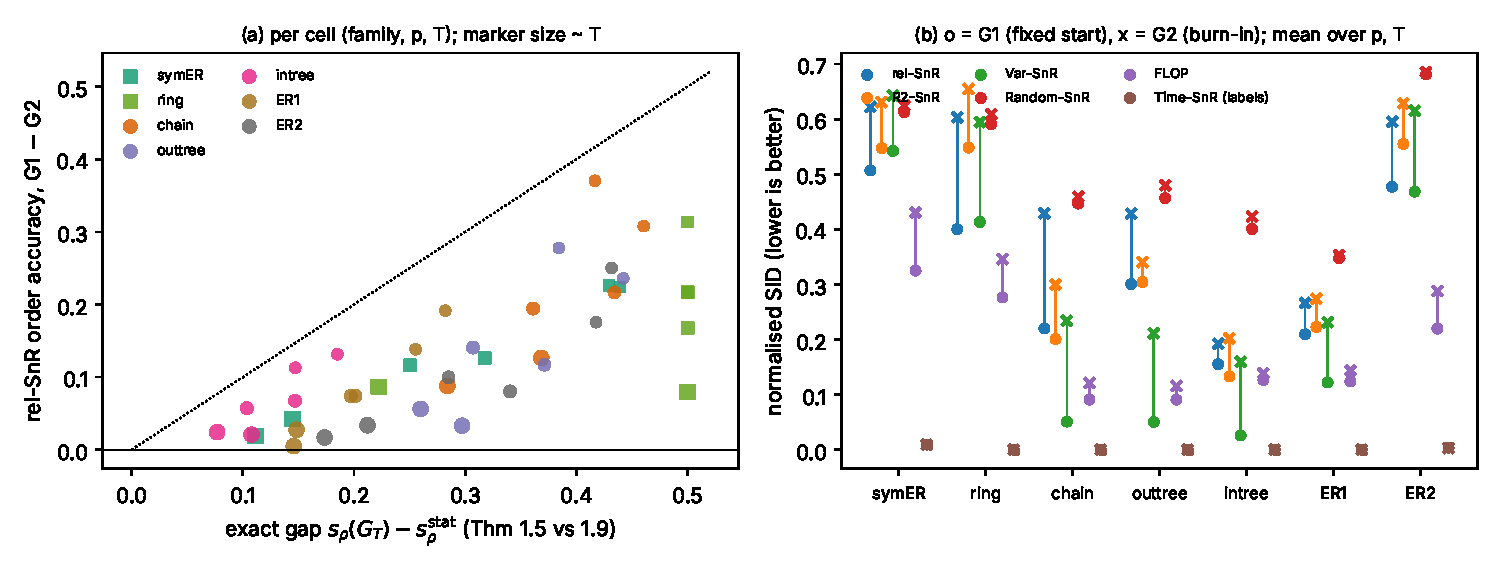
\includegraphics[width=0.48\linewidth]{figs/fig_b1.pdf}\hfill
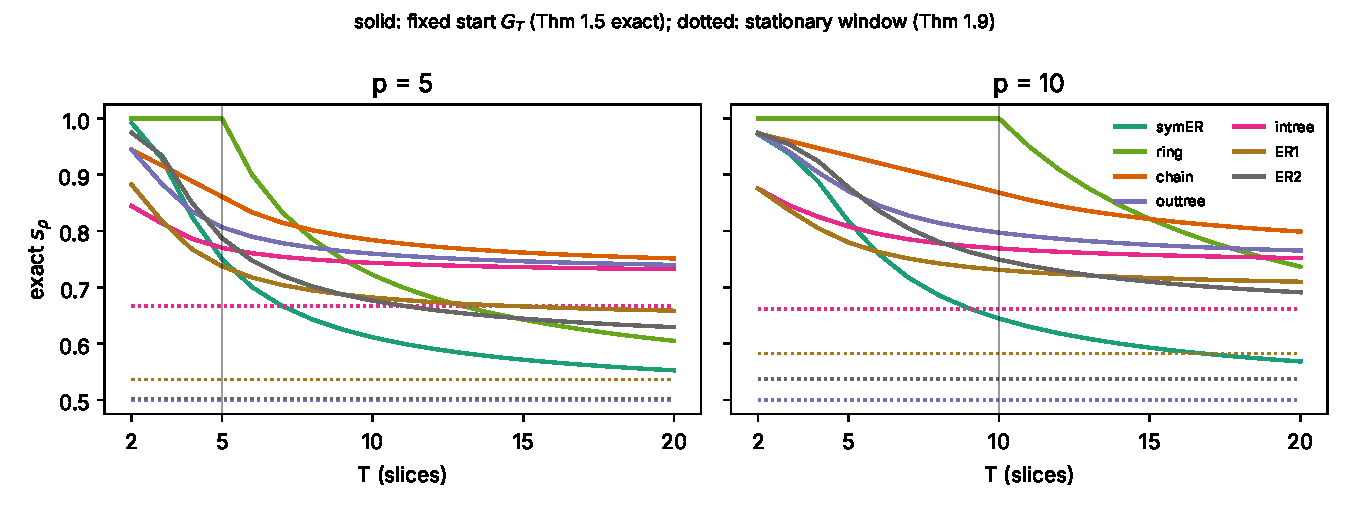
\includegraphics[width=0.48\linewidth]{figs/fig_srho_vs_T.pdf}
\caption{Left: per-cell G1$-$G2 gain in rel-SortnRegress order accuracy
against the exact population gap (all 42 cells below the diagonal and above
0), and normalised SID per method under G1 and G2. Right: exact
$\srho(\GT)$ against $T$, mean over the 30 test graphs per family and $p$.}
\label{fig:srhoT}
\end{figure}

\section{B1-NL: Replication under Nonlinear Dynamics, Signed Weights and Uniform Noise}
\label{app:b1nl}

\textbf{Process.} A separate plan (\texttt{b1nl/PLAN.md}) was committed before
any algorithm score; two notes (a faster but output-identical diagnostic, and
the limited power of sanity rule S1) were added after the validation run and
before the test run. No threshold, hypothesis or seed changed. The test run
(5{,}040 data sets) was run once.

\textbf{Design.} As B1 (\cref{app:b1}) with the B1 code imported unchanged:
seven families, $p\in\{5,10\}$, $T\in\{3,5,10\}$, $n=1000$, G1 against G2
(burn-in 100), R-het and R-std. Three parametrisations. NL: additive VAR with a
linear self-loop and cross terms $w\,g(x)$, $g$ drawn from $\tanh$, $\sin$ and
$(x+x^2/2)/(1+x^2/4)$, positive $w$, stability by scaling the Lipschitz-bound
matrix to spectral radius at most $0.8$. SGN: linear, all weights
$\pm\mathrm{Unif}(0.5,1)$. SGNU: SGN with uniform noise. New seeds (25 graphs per
family and $p$ for NL and SGN, 10 for SGNU); PC and R-eq dropped and G2s
replaced by a 500-step burn-in, to fit one core (stated in the plan).

\textbf{Results.} H1 (same rule as B1) supported in all three: 5/5 families
Holm-significant ($p\le1.4\cdot10^{-9}$); pooled gain $+0.108$ $[0.100,0.116]$
(NL), $+0.137$ $[0.128,0.146]$ (SGN), $+0.137$ $[0.123,0.152]$ (SGNU); positive in
all 126 cells. Tracking: Spearman $0.68$, $0.82$, $0.78$ (slopes $0.34$, $0.56$,
$0.56$). Under NL the correlation-count estimator recovers about $65\%$ of the
graph relatives (recall $0.67$ under G1, $0.62$ under G2), which explains the
smaller slope, as stated before the run. Under signed weights sample relatives
can deviate from graph relatives (out-trees under G2: estimated
rel-sortability $0.455$), yet the gain is as large as in B1. H3: one
Holm-significant SHD swap under NL ($R^2$-SortnRegress against the random order,
chains, $p=10$, $T=10$), none under SGN, not testable for SGNU (10 seeds, stated
in the plan). By the plan's rule H3 is therefore supported under NL, but on a
substantively minor swap, and we do not count it as a replication of B1's
swaps; B1's rel- against $R^2$-SortnRegress chain swap was not detected on SHD
at this replication's power, although the interaction replicates
(\cref{app:b1x}). Without PC, 5 of B1's 11 swap types cannot occur. FLOP is the
best label-free method run there under both generators in every configuration. The
var/rel split holds: Var-SortnRegress gains $+0.19$, $+0.24$, $+0.24$ raw and
about $0$ standardised; rel-SortnRegress $+0.11$, $+0.15$, $+0.14$. Sanity rules
pass (S1 at most $0.015$; mixing error at most $5.6\cdot10^{-5}$).

\begin{figure}[h]
\centering
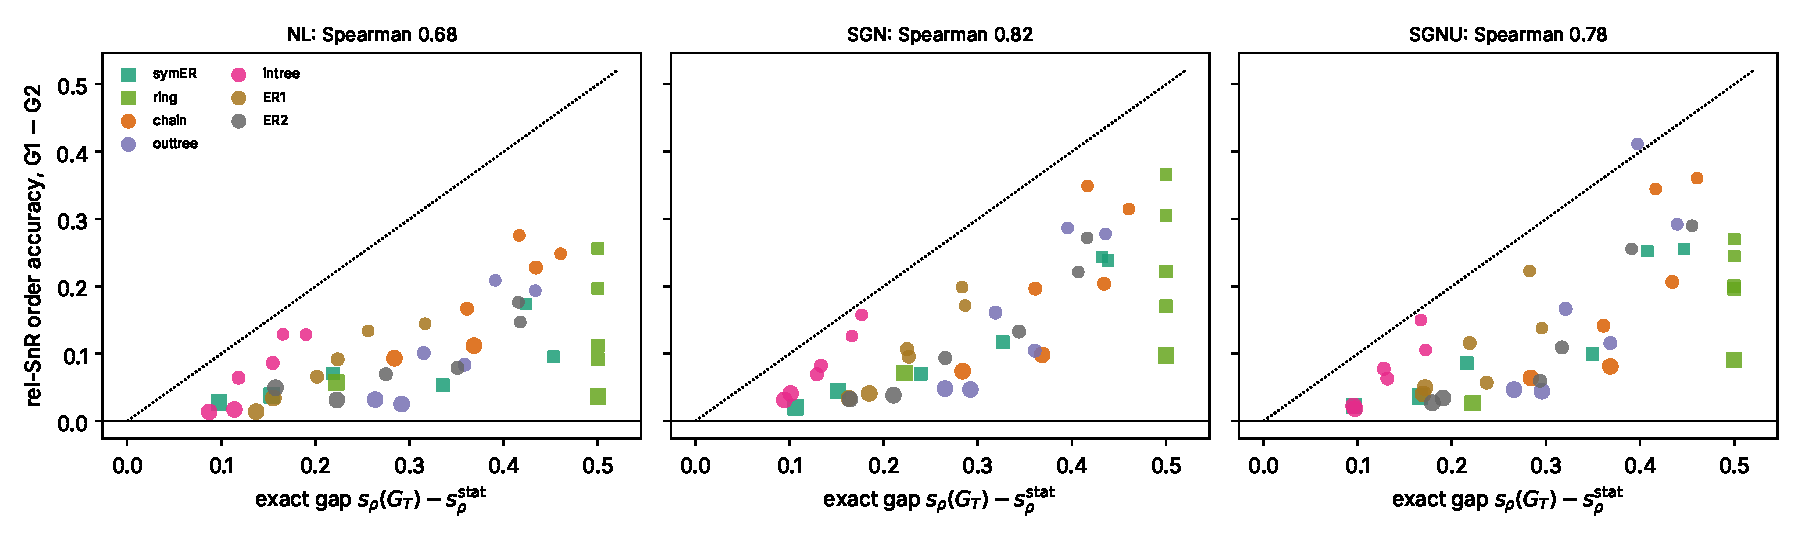
\includegraphics[width=0.7\linewidth]{figs/fig_b1nl.pdf}
\caption{B1-NL: per-cell G1$-$G2 gain in rel-SortnRegress order accuracy
against the exact population gap, for NL, SGN and SGNU.}
\label{fig:b1nl}
\end{figure}

\section{Competitive Learners, Re-Analysis, Detectability Oracle and Generator Survey}
\label{app:b1x}

Material in \texttt{b1x/} and \texttt{lit3/} of the supplement. The learner
extension is a planned experiment; the re-analysis and the oracle are post hoc
and use no new data.

\textbf{Learner extension: process and design.} The plan (\texttt{b1x/PLAN.md}),
code and a validation timing were committed and pushed before any score
(\cref{app:prereg}); the test run took 4.21\,h on one core and was analysed
once, with no deviation (the size rule kept 12 seeds after a projected 4.35\,h).
B1's generators and SEM, new seeds: families ring, chain, in-tree and
ER($c{=}2$), $p\in\{5,10\}$, $T\in\{3,5\}$, 12 graphs per (family, $p$), i.e.\ 96
summary graphs and 384 data sets (G1 and G2), each analysed raw and
standardised with time labels hidden. DAGMA linear (\texttt{dagma} 1.1.1,
$\lambda=0.03$), NOTEARS linear (the authors' reference code, $\lambda=0.1$),
GOLEM-EV/NV (a numpy port of the authors' code with the same score, optimiser,
defaults and post-processing, gradient-checked; $p=5$ only, as planned), all
thresholded at $0.3$; FLOP, the SortnRegress baselines and the empty graph as
comparators; PCMCI+ (tigramite, ParCorr, $\tau_{\max}=1$) on the time-indexed
data as a labels-using reference. Metrics: SHD$/|E|$ (empty graph $=1$),
normalised SID, ancestral order accuracy; unit of inference the summary graph.
T$=10$ and the families symER, out-tree and ER($c{=}1$) were excluded for run time.

\textbf{Verdicts.} HX1 (some raw continuous method Holm-significantly favoured
by the fixed start): supported; all four raw variants improve on all three
metrics (DAGMA SHD$/|E|$ $-0.548$ $[-0.663,-0.438]$, SID $-0.147$, order
accuracy $+0.197$; NOTEARS $-0.419$, $-0.127$, $+0.156$; GOLEM-EV $-0.491$,
$-0.182$, $+0.225$; GOLEM-NV $-0.409$, $-0.193$, $+0.232$; Holm $\le4\cdot10^{-8}$).
HX2 (opposite-sign, both Holm-significant rank change against FLOP on
SHD$/|E|$, 64 tests): supported, two changes, both on in-trees: DAGMA$-$FLOP
$-0.218$ under G1 (Holm $0.012$) and $+0.306$ under G2 ($1.4\cdot10^{-5}$);
NOTEARS$-$FLOP $-0.176$ ($0.0011$) and $+0.193$ ($0.020$); the same two appear on
SID and order accuracy, and DAGMA's persists without first-slice pairs ($0.08$ /
$0.73$ against FLOP's $0.30$ / $0.37$). HX3 (standardisation removes the gain):
DAGMA's SHD gain removed ($-0.005$ $[-0.027,0.016]$), all other pairs reduced
but not removed by the plan's rule; on order accuracy the standardised effect is
significantly negative for DAGMA ($-0.064$), GOLEM-EV ($-0.093$) and GOLEM-NV
($-0.097$), and NOTEARS keeps $+0.036$. rel-SortnRegress replicates ($+0.187$
$[0.169,0.205]$), and B1's chain swap of rel- against $R^2$-SortnRegress recurs
on the new seeds. No fit failed; NOTEARS on standardised data returned a cyclic
graph in $15.6\%$ of data sets (SID missing for 60 of 384). Best label-free
method by mean SHD$/|E|$ per (family, $p$): FLOP in 8/8 cells under G2; under G1
DAGMA on chains with $p=5$ ($0.09$ vs $0.10$) and on in-trees with $p=10$ ($0.06$ vs
$0.33$), NOTEARS on in-trees with $p=5$ ($0.09$ vs $0.27$). Raw continuous methods
beat the empty graph on average under both generators but are worse than it
on chains under G2 ($1.14$--$1.25$). Standardised DAGMA and GOLEM orient most
tree edges backwards under G1 (order accuracy $0.26$--$0.27$). The gains and
the reversals are largest on chains and in-trees, where G1 makes the window
almost perfectly var-sortable (Var-SortnRegress $0.95$--$0.96$), and absent or
reversed on rings and ER($c{=}2$). This is consistent with a var-sortability
effect, but the experiment does not establish it.

\textbf{Predictions of the plan and what the attribution rests on.} The plan
stated three predictions. For HX1 it predicted favourable effects on raw data
for all continuous methods; this held. For HX2 it predicted no rank change
against FLOP on SHD$/|E|$; this failed (two changes). For HX3 it predicted
``reduced, not removed'' for DAGMA and NOTEARS on order accuracy, because some
scale-free gain should survive standardisation. By the plan's rule both were
labelled ``reduced, not removed'', but for DAGMA the standardised effect is
negative ($-0.064$), so no gain survives; for NOTEARS a gain survives
($+0.036$ order accuracy, $-0.077$ SHD$/|E|$, $-0.073$ SID, all
Holm-significant). The standardised runs are a weak test of the attribution
to var-sortability. Standardised DAGMA and GOLEM have order accuracy below
$1/2$ under both generators (DAGMA $0.35$ / $0.41$, GOLEM $0.31$--$0.33$ /
$0.41$--$0.42$), so they cannot show a scale-free effect of either sign.
NOTEARS's remaining gain is a scale-free start effect on a competitive
method. The fixed start also raises $R^2$-sortability, which is scale free
and outside our theory, and we did not separate it. In B1 the gain in
Var-SortnRegress order accuracy is the same on rings ($+0.224$) and chains
($+0.231$), while the learners gain on chains and not on rings; the
explanation by levels ($0.73$ against $0.93$ under G1) was made after the
results. A control that rescales each data set to the other generator's
marginal variances would test the attribution; it has not been run. GOLEM
did not overtake FLOP on in-trees (G1 differences $-0.011$ and $-0.042$, Holm
$1$ and $0.46$). \Cref{tab:b1x} omits GOLEM-EV (SHD$/|E|$ $0.44$ / $0.93$ raw)
and standardised GOLEM ($0.97$ / $1.30$ EV, $0.95$ / $0.99$ NV).

\textbf{Re-analysis of B1 and B1-NL (post hoc).} Graph-cluster bootstrap CIs
(10{,}000 resamples, the three horizons of a graph kept together) are narrower
than data-set bootstrap CIs, because $T$ is a fixed design
factor; they are used in \cref{tab:b1}. Tracking: cell-level Spearman $0.80$
$[0.76,0.82]$, unit-level $0.62$ $[0.59,0.64]$, slope $0.53$ $[0.50,0.56]$ in B1;
$0.68$/$0.44$/$0.34$ (NL), $0.82$/$0.64$/$0.56$ (SGN), $0.78$/$0.62$/$0.56$ (SGNU);
graph-cluster permutation $p\le10^{-4}$ in all four (the floor). Interactions
$I=[m_1-m_2](\mathrm{G1})-[m_1-m_2](\mathrm{G2})$ per graph: Holm-significant in
294/595 (B1), 113/420 (NL), 232/420 (SGN) pair$\times$cell SHD tests and 0 for
SGNU (10 graphs cannot pass Holm). In-tree Var-SortnRegress$-$FLOP on SHD:
$-68.4$ $[-77.0,-60.4]$ (B1), $-49.9$ (NL), $-75.5$ (SGN), $-75.5$ (SGNU); SID
$-0.12$ in all four. Chain rel-$-R^2$-SortnRegress: SID and orientation
interactions replicate at $60$--$80\%$ of B1's size; the family-pooled SHD
interaction is about $0$ in B1-NL, but in B1's swap cell ($p=10$, $T=3$) it keeps
its sign ($-52$, $-16$, $-32$). Empty-graph reference (B1, all families, G1 / G2,
SHD$/|E|$): rel- $1.05$/$1.70$, $R^2$- $1.33$/$1.96$, Var- $0.61$/$1.39$,
random $1.72$/$2.04$, FLOP $0.27$/$0.46$, PC $0.40$/$0.64$; the empty graph has
normalised SID $0.50$. Order accuracy without edges leaving the first window
slice (non-SC families): rel-SortnRegress $+0.089$ $[0.079,0.100]$ (B1), $+0.067$
(NL), $+0.087$ (SGN), $+0.095$ (SGNU). Multiplicity: each claim of
B1, B1-NL, B3 and the extension gets one claim-level $p$ (the $k$-th smallest
Holm $p$ for ``$k$ of $m$ families'' rules, the best swap for swap rules, the
cluster permutation for tracking, the plan's Holm $p$ for B3); Holm over the 21
claims at family-wise $0.05$ keeps all but B1-NL H3-SGN ($p=0.108$); the closest
survivors are B1 H3 (Holm $0.0079$), B1-NL H3-NL and HX2 (both $0.033$). Several
claim $p$ are at resolution floors ($10^{-4}$ for permutations, $10^{-5}$ for
B3's sign flips).

\textbf{Detectability calculation (``oracle''; post hoc).} For every B1 test graph, parameter set
and horizon we propagated the exact window covariance (G1:
$\Sigma_{t+1}=A^\top\Sigma_tA+D$ from $\Sigma_1=D$; G2: after the same 100
burn-in steps). Population relatives ($|\rho|>10^{-20}$) reproduce the exact
$\srho$ of \cref{thm:limit,thm:stat} in all 2{,}520 cases. The oracle replaces
each sample correlation in rel-SortnRegress's count by the probability that
the Fisher-$z$ statistic at $n=1000$ exceeds the algorithm's threshold
($\varepsilon=0.062$) and predicts each edge's order accuracy as
$P(c_i<c_j)+\tfrac12P(c_i=c_j)$, treating the indicators as independent. It uses
no simulated data. Against the observed G1$-$G2 gain: cell level Spearman
$0.99$, $R^2=0.97$, slope $1.03$, intercept $-0.010$; unit level $R^2=0.61$
against $0.34$ for the exact gap (difference $+0.27$ $[0.23,0.30]$); in a joint
regression the gap's coefficient is $-0.063$ over cells and $-0.039$ over graph--horizon units. Predicted G1 / G2 levels: chain
$0.756$/$0.528$ (observed $0.749$/$0.532$), ring $0.702$/$0.503$ ($0.687$/$0.507$),
in-tree $0.746$/$0.677$ ($0.743$/$0.673$). Without slice-1 edges the non-SC gain
is predicted to fall from $+0.130$ to $+0.096$ (observed $+0.125$ to $+0.089$).
What this shows and does not show: the calculation is the expectation of
rel-SortnRegress under the exact covariances of each generator, so the
agreement says that the simulated gain has the size those covariances imply
and that the independence approximation is adequate. It uses the full
start-dependent covariances, so it includes every way in which the start
changes pairwise correlations: pairs that are relatives under the fixed start
only (the mechanism of \cref{sec:exact}) and pairs that are relatives under
both starts but differ in correlation strength (a transient that needs no
graph argument). We did not decompose the predicted gain into these two
parts, so the calculation does not show that the gain is due to the first.
The exact gap therefore gives a ranking and a rough scale; all 42 cells have the same sign, so the sign tests nothing.

\textbf{Generator survey.} We read the source code of tigramite 5.2.10.1
(\texttt{structural\_causal\_process}: zeros plus noise, burn-in
$\lfloor0.2T\rfloor$; \texttt{var\_process}: i.i.d.\ $N(0,1)$ start, no burn-in),
the CDML generator \citep{lawrence2021dgp} (zeros, $2\tau_{\max}$ steps dropped),
CausalTime \citep{cheng2024causaltime} (rollouts of 20 steps from a real-data
window, no burn-in, in the demo), UUMCdata \citep{herman2025unitless} (exact
stationary start), causalnex 0.12.1 (zeros, burn-in 100 or more; data with lag
labels), the Neural-GC VAR and Lorenz-96 simulators \citep{tank2021neural}
(burn-in 100 and 1000) and gCastle 1.0.4 (no continuous time-series
simulator; its Hawkes simulator starts with an empty history). cdt, causaldag,
causal-learn and lingam ship no time-series benchmark generator.
\citet{lohse2025sortability} state a burn-in without its length. The
time-unrolled construction of \citet{reisach2026topological} starts at $t=1$
and gives every slice to an i.i.d.\ method as a separate variable; its code is
not public, so only the graph-level start is verified. CauseMe's documentation
could not be opened with TLS verification, so we make no claim about it. File
and line references are in \texttt{lit3/GENERATOR\_SURVEY.md}. Reading of
exposure: the burn-in lengths above can be compared with
$\Delta\tau_{\max}$, which concerns the graph artefact only. The variance
artefact needs the start to be far from the stationary distribution relative
to the mixing time of the process, which depends on the spectral radius of
the generated coefficients; we computed no mixing time for any of these
generators, so we do not grade them on it. All of them except the
time-unrolled construction produce a single record with time order for
time-series methods, so neither artefact applies to them as shipped; they
would be exposed only if windows from their first steps were given to a
method that ignores time order.

\section{B3: Discriminating Test of the Source-SCC Rule on Held-Out Data}
\label{app:b3}

\textbf{Process.} The plan (\texttt{b3/PLAN.md}, with an OSF-formatted copy) was
pushed before any byte of the held-out data was read; zip CRC-32 values were
taken from the remote archive directory before the plan and SHA-256 hashes at
download. The plan is internally time-stamped only: it was not posted to an
external registry before data access, and results were committed 3--4 minutes
after the plan. A disclosed development check on study-3 data from the same
device had shown every colour edge to be detectable, so the primary outcome
was expected.

\textbf{Data.} Causal Chambers experiments not previously downloaded by the
project. H1 (primary): \texttt{lt\_camera\_walks\_v1}, experiments
\texttt{ar\_1\_uniform\_\{ref, pol\_1\_90, pol\_12\_30\}}: five independent
stationary AR(1) actuators drive the light sensors, so the colour block is
one weak component with three source SCCs; $3\times30{,}000$ steps, 30 units of
3{,}000. H2 (co-primary): \texttt{lt\_camera\_v1/scm\_5\_red} and
\texttt{scm\_5\_blue}, i.i.d.\ data from the collider R$\to$G$\leftarrow$B, 20
units. Secondary: \texttt{scm\_5\_green}, \texttt{scm\_4\_green},
\texttt{scm\_4\_blue}, and \texttt{scm\_4\_red} as a single-source control.

\textbf{Test.} E1's estimator unchanged. Competitors: constant $1/2$, the
weak-component-size rule, the theorem on the design graph $G_D$, and E1's
eight naive rules. Primary set $D^*$: instances where the theorem and the
weak-component rule disagree ($56\%$ of instances for H1, $47\%$ for H2, from
graph-only computation before the plan); on $D^*$ the prediction is the same
on $G_{\mathrm{lin}}$ and $G_D$. Failure of the estimator pushes observed values
towards the tie rules, so a pass on $D^*$ cannot come from ties. Sign-flip
tests over units, Holm, family $\alpha=0.025$; pass requires $\Delta\le-0.10$
against every competitor that disagrees on $D^*$.

\textbf{Results.} H1: on 2{,}361 instances, counts sorted as predicted in
2{,}356; $\Delta=-0.498$ against both tie rules, 30/30 units, $p\approx10^{-5}$;
non-relatives declared dependent $0.054$, relatives detected $0.990$. H2:
$\Delta=-0.50$ against the tie rules and the sensor indicator, 20/20 units;
R$\to$G sorted 264/264 when B is observed and tied 123/123 when not. S1
(predicted tie, detected edge; 1{,}251 instances): theorem beats the eight
naive rules ($\Delta=-0.43$, 30/30 units) and the theorem on $G_D$ narrowly
($\Delta=-0.21$, 21/30 units, Holm $p=0.021$). No stop condition met.

\textbf{Failures.} \texttt{scm\_4\_blue}: the tie rule is significantly better
($\Delta=+0.115$, 0/10 units, reverse $p=0.001$); post hoc, the intervened blue
channel ranges over 1--13 of 255 levels, so none of its edges is detected, and
the pooled detection prerequisite ($0.837$) did not catch this. The pooled
secondary analysis still passes, in 20/30 units. In
\texttt{ar\_1\_uniform\_pol\_1\_90} the polariser linear-zero refinement of
\cref{app:e1} fails (polarisers correlate with ir$_3$, vis$_3$ at
$|r|\approx0.2$--$0.28$; $G_D$ matches $0.959$ against $0.041$ for
$G_{\mathrm{lin}}$); H1 does not depend on it. Deviations: the inputs of two
experiments do not reproduce from the published generator seeds (ranges
match; not gating).


%=============================================================================
\section{Proofs for Sections~\ref{sec:labels} and~\ref{sec:ident}}
\label{app:ident}

\Cref{prop:nogain} is proved in the main text. The proofs below are paper
proofs; none is machine-checked. Notation as in \cref{sec:ident}.

\begin{proof}[Proof of \cref{prop:slices}]
(a) Every edge of $\GT$ goes from a slice $t$ to slice $t+1$, so a directed
path ending in $v(t)$ has at most $t-1$ edges, and the self-chain
$v(1)\to\dots\to v(t)$ has exactly $t-1$. Graph isomorphisms preserve height,
so two labellings of the same column DAG as unrollings with self-loops put the
same columns in slice $t$, and $T$ is the largest height and $p$ the number of
columns of height one.
(b) The column DAG of the ring $i\to i+1$ with self-loops has the edges
$(i,t)\to(i,t{+}1)$ and $(i,t)\to(i{+}1,t{+}1)$. With the new unit label
$i'=i-t \pmod p$ the first family reads $i'\to i'-1$ and the second
$i'\to i'$, which is the unrolling of the reversed ring with self-loops.
(c) Without loops the unrolling of $0\to1$ has the edges $0(t)\to1(t{+}1)$,
$t<T$, which are pairwise disjoint; every one of them has a tail of height one
and a head of height two.
\end{proof}

\begin{proof}[Proof of \cref{prop:mec}]
Two parents $i(t)$ and $k(t)$ of a node $j(t{+}1)$ lie in the same slice and
are not adjacent, so every node with at least two parents is an unshielded
collider, and all its incoming edges have the same direction in every member
of the class. The remaining edges are those into nodes with exactly one
parent; since every node $j(t{+}1)$ has the parent $j(t)$, these are the
self-chain edges of loop-only units. Fix such a unit $j$ and a member of the
class. On the chain $j(1),\dots,j(T)$ the member has no collider (a collider
at a chain node would be unshielded, as chain neighbours at distance two are
not adjacent, and $\GT$ has none there), so the chain is oriented away from
one of its nodes $j(s)$. Conversely, re-rooting the chain at any $j(s)$ keeps
the skeleton, creates no collider (every chain node still has at most one
parent, because a loop-only unit has no parent outside its chain), removes
none, and creates no cycle (a directed cycle would have to enter the chain
from outside, and no edge does). The chains of different loop-only units are
disjoint and can be re-rooted independently, which gives $T^{m_0}$ members.
\end{proof}

\begin{proof}[Proof of \cref{prop:fixident}]
(a) Let $G'$ be the column DAG of a sparsest representation. $\Sigma$ is
Markov to $G'$, because the representation is a linear structural equation
model on $G'$ with independent noise terms (the start covariance is diagonal
under the fixed-start law). $G'$ has $(T-1)|\mathrm{supp}\,A'|$ edges, at most
as many as $\GT$, because the true parameter is itself a representation. As
the distribution is faithful to $\GT$, a DAG to which it is Markov has at
least as many edges as $\GT$, with equality only if it is Markov equivalent
to $\GT$ \citep[Theorem~4]{chickering2002optimal}. By \cref{prop:mec}, $G'$ is
$\GT$ with the chains of some loop-only units re-rooted. $G'$ is also an
unrolling with self-loops, so by \cref{prop:slices}(a) every edge of $G'$
joins consecutive heights, and every node of height at least two has a
self-parent, with different nodes having different self-parents. Re-root the
chain of a loop-only unit $j$ at $j(s)$. If $1<s<T$, then $j(s)$ has no parent
in $G'$, and $j(s{-}1)$ and $j(s{+}1)$ both have $j(s)$ as their only parent,
so both would have the self-parent $j(s)$: impossible. If $s=T$, then $j(1)$
has height $T$ in $G'$; if $j$ has a child $k\ne j$ in $\GS$, the edge
$j(1)\to k(2)$ is an edge of $G'$ (it enters a node with two parents or more,
namely $j(1)$ and $k(1)$), which gives $k(2)$ the height $T+1$: impossible. So
only isolated units can be reversed, and only as a whole.
(b) Let $v_t$ be the variance of $x_j(t)$, $v_{t+1}=a^2v_t+d$. The reversed
chain is a representation iff the regression of $x_j(t)$ on $x_j(t{+}1)$ has
the same coefficient $a v_t/v_{t+1}$ and the same residual variance
$d\,v_t/v_{t+1}$ for all $t\in\{1,\dots,T-1\}$, i.e.\ iff $v_t/v_{t+1}=r$ does
not depend on $t$. For $T=2$ there is one transition and nothing to compare.
For $T\ge3$, $v_3-v_2=a^2(v_2-v_1)$ gives
$\tfrac1r(\tfrac1r-1)=a^2(\tfrac1r-1)$, so $r=1$, which is stationarity, or
$1/r=a^2$, which forces $d=0$ and is excluded. If $r=1$ for the first two
transitions then $v_t$ is constant for all $t$.
(c) follows from (a) and (b).
\end{proof}

\begin{proof}[Proof of \cref{prop:nonident}]
(a) In the truth, $a_2=\alpha a_1+\varepsilon_a$ and
$b_2=\beta a_1+\gamma b_1+\varepsilon_b$, with an arbitrary covariance of
$(a_1,b_1)$. Take the units $a'=(a_1,a_2)$ and $b'=(b_2,b_1)$, i.e.\ the first
slice $\{a_1,b_2\}$ and the second slice $\{a_2,b_1\}$. Then
$a_2=\alpha a_1+0\cdot b_2+\varepsilon_a$ and $b_1=\beta'a_1+\gamma'b_2+\eta$,
where $\eta$ is the residual of the linear regression of $b_1$ on
$(a_1,b_2)$. By construction $\eta$ is uncorrelated with the new first slice;
it is a linear function of $(a_1,b_1,\varepsilon_b)$ and therefore
uncorrelated with $\varepsilon_a$, and $\varepsilon_a$ is uncorrelated with
$(a_1,b_2)$. So the new innovation covariance is diagonal and uncorrelated
with the new first slice, whose covariance is free. The new self-loop
coefficients are $\alpha\ne0$ and $\gamma'$, which is non-zero whenever
$\gamma\ne0$ (the partial correlation of $b_1$ and $b_2$ given $a_1$ is
non-zero); the support of the new transition matrix has three entries when
$\beta'\ne0$ and two otherwise, so the new representation has no more edges
than the truth.
(b) A stationary Gaussian AR(1) process has a symmetric autocovariance, so
the reversed window has the same covariance, and an isolated unit is
uncorrelated with all other columns.
(c) $\Gamma=\sigma^2(I-A^2)^{-1}$ solves $\Gamma=A\Gamma A^\top+\sigma^2I$ and
commutes with $A$. The time-reversed stationary process has transition matrix
$\Gamma A^\top\Gamma^{-1}=A$ and innovation covariance
$\Gamma-A\Gamma A^\top=\sigma^2I$, so the reversed window is a representation
with the same support.
\end{proof}

\textbf{On \cref{conj:window}.} Let $H$ be $\GT$ plus a complete DAG on the
first slice. Under the stated faithfulness, the argument of
\cref{prop:fixident}(a) shows that the DAG of a sparsest representation (its
unrolling plus a complete DAG on its first slice) is Markov equivalent to $H$,
hence has the same skeleton $U$. In $H$ the edges between slices 1 and 2 are
not fixed by colliders, because the parents of a slice-2 node lie in the
first-slice clique. If the only partition of the nodes of $U$ into $T$ layers
of size $p$, with edges inside layer 1 or between consecutive layers and a
perfect matching between consecutive layers, is the true one, the conjecture
follows; the reversed layering is excluded when slice $T$ is an independent
set of $U$ and slice 1 is not. We checked uniqueness by hand for the summary
edge $a\to b$ with self-loops and $T=3$; \cref{prop:nonident}(a) shows that it
fails for $T=2$. We have no proof for general graphs, and the case in which
the first slice is not a clique in $U$ is not covered.
